%
% The first command in your LaTeX source must be the \documentclass command.
\documentclass[sigconf]{acmart}

%
% defining the \BibTeX command - from Oren Patashnik's original BibTeX documentation.
\def\BibTeX{{\rm B\kern-.05em{\sc i\kern-.025em b}\kern-.08emT\kern-.1667em\lower.7ex\hbox{E}\kern-.125emX}}
    
% Rights management information. 
% This information is sent to you when you complete the rights form.
% These commands have SAMPLE values in them; it is your responsibility as an author to replace
% the commands and values with those provided to you when you complete the rights form.
%
% These commands are for a PROCEEDINGS abstract or paper.
\copyrightyear{2018}
\acmYear{2018}
\settopmatter{printacmref=false}
\setcopyright{acmlicensed}
\acmConference[Woodstock '18]{Woodstock '18: ACM Symposium on Neural Gaze Detection}{June 03--05, 2018}{Woodstock, NY}
\acmBooktitle{Woodstock '18: ACM Symposium on Neural Gaze Detection, June 03--05, 2018, Woodstock, NY}
\acmPrice{15.00}
\acmDOI{10.1145/1122445.1122456}
\acmISBN{978-1-4503-9999-9/18/06}
%\usepackage{cite}
%\usepackage[bottom]{footmisc}
\usepackage{enumitem}
\usepackage{amsmath,amssymb,amsfonts}
\usepackage{algorithm}
%\usepackage{hyperref}
%\usepackage{algorithmic}
\usepackage{algcompatible}
\usepackage{graphicx}
\usepackage{comment}
\usepackage{multirow} 
\usepackage{amsthm}
\usepackage{textcomp}
\usepackage{xcolor}
\def\BibTeX{{\rm B\kern-.05em{\sc i\kern-.025em b}\kern-.08em
    T\kern-.1667em\lower.7ex\hbox{E}\kern-.125emX}}
\usepackage{amsmath}

\usepackage{xspace}
\usepackage{caption}
\captionsetup[figure]{font=small,labelfont=small}
\usepackage{subcaption}
\captionsetup[subfigure]{font=scriptsize,labelfont=scriptsize}
\newtheorem{theorem}{Theorem}
\newtheorem{definition}{Definition}
\newtheorem{exmp}{Example}[section]
\usepackage{mathtools}
\DeclarePairedDelimiter\ceil{\lceil}{\rceil}
\DeclarePairedDelimiter\floor{\lfloor}{\rfloor}
\usepackage{xspace}


\newcommand{\eat}[1]{}
\newcommand{\am}[1]{{\color{blue} \emph{[[AM: #1]]}}}
\newcommand{\arc}[1]{{\color{blue} \emph{[[ARC: #1]]}}}
\newcommand{\xh}[1]{{\color{purple} \emph{[[XH: #1]]}}}


\newcommand{\stitle}[1]{\vspace{.33em}\noindent\textbf{#1}~}

\newcommand{\system}{Crypt$\epsilon$\xspace}

\newcommand{\encD}{\boldsymbol{\tilde{\mathcal{D}}}}
\newcommand{\crossproduct}{\times}
\newcommand{\project}{\pi}
\newcommand{\filter}{\sigma}
\newcommand{\countagg}{count}
\newcommand{\groupbystar}{\gamma^{*,count}}
\newcommand{\groupby}{\gamma^{count}}
\newcommand{\countdistinct}{count^*}
\newcommand{\encT}{\boldsymbol{\tilde{T}}}
\newcommand{\encB}{\boldsymbol{B}}
\newcommand{\encC}{\boldsymbol{c}}
\newcommand{\encV}{\boldsymbol{V}}
\newcommand{\lap}{Lap}
\newcommand{\noisymax}{NoisyMax}
\newcommand{\postorder}{post}

\newcommand{\squishlist}{
	\begin{list}{$\bullet$}
		{
			\setlength{\itemsep}{0pt}
			\setlength{\parsep}{3pt}
			\setlength{\topsep}{3pt}
			\setlength{\partopsep}{0pt}
			\setlength{\leftmargin}{1.5em}
			\setlength{\labelwidth}{1em}
			\setlength{\labelsep}{0.5em} } }
	
\newcommand{\squishend}{
\end{list}  }

\hypersetup{draft}


\begin{document}
\title{\system: Crypto-Assisted Differential Privacy on Untrusted Servers}
\author{}
\begin{abstract}
Differential privacy has steadily become the de-facto standard for achieving strong privacy guarantees in data analysis. It is typically implemented either in the ``central" or ``local" model. In the former, a trusted centralized server collects the records \textit{in the clear} from the data owners in the clear and outputs differentially private statistics; while in the latter, the data owners individually randomize their inputs to ensure differential privacy.  The local model has been popular as it dispenses with the need for a trusted data collector. This increased security in the local model, however, comes at the cost of strictly lower accuracy and restricted algorithmic expressibility for differentially private programs compared to the central model. 

In this work, we propose, \system, a  system for differential privacy that (1) eliminates the need for a trusted data collector like in the local model, but still (2) achieves the accuracy guarantees and algorithmic expressibility of DP programs of the central model. \system achieves this "best of both worlds" result by employing two non-colluding untrusted servers that run differentially private programs on encrypted data from data owners. \system 
supports a rich class of differentially private programs that can be written in terms of a small set of primitives inspired by relational algebra. Further, we propose optimizations that speed up computation on encrypted data by leveraging the fact that the final output is differentially private. We demonstrate the feasibility of \system for practical differentially private analysis on untrusted servers with an extensive empirical evaluation on real datasets.
\end{abstract}
\begin{CCSXML}
<ccs2012>
<concept>
<concept_id>10002978.10002979.10002981.10011745</concept_id>
<concept_desc>Security and privacy~Public key encryption</concept_desc>
<concept_significance>300</concept_significance>
</concept>
<concept>
<concept_id>10002978.10002991.10002995</concept_id>
<concept_desc>Security and privacy~Privacy-preserving protocols</concept_desc>
<concept_significance>300</concept_significance>
</concept>
</ccs2012>
\end{CCSXML}
\ccsdesc[300]{Security and privacy~Public key encryption}
\ccsdesc[300]{Security and privacy~Privacy-preserving protocols}
%\begin{IEEEkeywords}

\keywords{Differential Privacy, Crypto Service Provider, Linear Homomorphic Encryption}
 \settopmatter{printfolios=true}
\maketitle
%\end{IEEEkeywords}
\section{Introduction}

\eat{\am{Outline of the intro: 
\begin{itemize}
	\item Para 1: Consensus on DP/informal definition
	\item Para 2 :Two models of implementation -- central vs local. Informally define the models. Not sure if you need to go into Laplace random variables or binomial random variables. 
	\item Para 3: LDP is popular in some deployments due to security ... 
	\item Para 4: Utility cost: use lower bounds rather than upper bound results for LDP. I see a $O()$ ... should use $\Omega()$. A better way to do this would be to first discuss the lower bounds, and then give an example of a simple count query and show how the separation works. In particular, you can answer a count query using Laplace mechanism in the central model with $O(1/\epsilon)$, but you need $\Omega(\sqrt{n}/\epsilon)$ noise for the LDP model. Read the Adam smith/Ulfar papers on the anonymous channels to see how this is written in other papers. 
	\item Para 5: In this paper we present a system that uses cryptography to bring the gap ...: See how I wrote the abstract and rewrite this para. Say one line about how this is in line with a growing line of literature that is using crypto to address the trust assumptions in central model [citations] (see related work section for details). Also, when you first say two-server model, give a bunch of citations to the crypto-assisted model. 
	\item Contributions: see comments later on.   
\end{itemize}}}

%Thre has been a growing consensus to papers like Contributions of our work is three fold%$\begin{enumerate}\item we have by achieving the \end{enumerate}
%Differential privacy has steadily emerged as a compelling privacy definition in situations when aggregate statistics must be released from databases without revealing properties of individual records. %that allows us to glean useful information about data alongside providing privacy at the granularity of individuals. %Formal privacy guarantees in tandem with quantifiable utility-privacy trade-offs have been instrumental in making it the de-facto standard for achieving data privacy.
%An algorithm satisfies differential privacy if adding or removing a single record from its input does not significantly change its output \cite{dwork}. This is a compelling guarantee as it bounds the additional privacy risk to any individual record  % It is essentially a property of a function such that its output should disallow any inference about the presence (or absence equivalently) of any individual record in its input data set \cite{dwork}. Formally, it requires that for any outcome of a randomized function, that outcome should be nearly equally likely with and without any one record. 

In several domains, including social science, healthcare, and advertising, there is growing need for releasing aggregate properties from sensitive datasets. Differentially private algorithms \cite{dwork}, whose outputs are insensitive to adding or removing a single row in the input dataset, have arisen as the gold standard for these situations. Differential privacy provides a provable and persuasive guarantee of privacy to individuals in a dataset, and has seen adoption in government \cite{machanavajjhala08onthemap,Vilhuber17Proceedings} and commercial organizations \cite{Rappor1,Apple}. It is defined with respect to a privacy parameter $\epsilon > 0$ where lower the value of $\epsilon$, greater is the privacy guarantee obtained.

Differential privacy (DP) is typically implemented in one of two models -- \textit{centralized differential privacy}, or \textsf{CDP}, and \textit{local differential privacy}, or \textsf{LDP}. In \textsf{CDP}, data from individuals are collected and stored \textit{in the clear} in a \textit{trusted} centralized data curator. The trusted curator executes DP programs on the sensitive data  and releases outputs to a mistrustful data analyst. A canonical algorithm in \textsf{CDP} is the Laplace mechanism where the curator releases the output of a function $f$ by adding noise drawn from the Laplace distribution to hide the presence or absence of one row in the input database. 

%Depending on infrastructural constraints, like the viable trust model in a given setting, differential private algorithms in practice can have two different styles of implementation.  The more common and historically precedent implementation is the central differential privacy (\textsf{CDP}) model where a trusted data curator collates data from all individuals into a centrally held dataset and processes it in a privacy preserving way. %For example, the data curator could publish differentially private statistics of the data, that allows analysis on the data, without revealing individual information. 
%The curator is trusted to store the data \emph{in the clear} and mediates upon queries posed by a mistrustful analyst, interested in learning some synopsis of this dataset. Privacy is enforced by the curator by adding uncertainty to the answers for analyst's queries before releasing them. The other competing model of implementation, is the local differential privacy model (\textsf{LDP}) where the central data aggregating server is untrusted. Thus every data owner has to individually randomize his/her input before communicating it to the central aggregator. Hence the private data is concealed from the untrusted aggregator who attempts to infer statistics about the true population from the perturbed data instead. 

In \textsf{LDP}, there is no trusted centralized data curator. Rather, each individual perturbs their own data using a (local) differentially private algorithm. The data analyst has direct access to these perturbed data, and uses it to infer aggregate statistics of the datasets. A canonical LDP algorithm is the randomized response mechanism \cite{RR} where each data owner flips some of his/her input bits based on a coin toss to provide \emph{plausible deniability} \cite{Dork}.


 \par  \textsf{LDP}'s non-reliance on any trusted third party  gives it an edge over \textsf{CDP}. It is so because firstly, \textsf{CDP}'s assumption of a trusted server is very strong and ill-suited for many practical scenarios. Secondly, a single point of data breach in \textsf{CDP} can be catastrophic for the entire dataset. Moreover, in the wake of stringent data protection regulations like \textsf{GDPR}, \textsf{HIPAA} etc, a trusted data curator is saddled with legal and ethical obligations to uphold the privacy of its data, making its practical implementation to be cumbersome.
  
 %Most notable use cases for LDP include observing most frequent software features and measuring their performance and failure characteristics; collecting data about users' default browser homepage and search engine et al.  
 \par Regrettably, this ease of adopt-ability for \textsf{LDP} comes with an utilitarian price tag. Specifically, computation in \textsf{LDP} results in an additional error of $\Omega(\sqrt{n})$ where $n$ is the total number of data owners contributing to the noisy estimate \cite{error1,error2,error3}. In contrast, we get a constant error bound for \textsf{CDP}.
For e.g., for a single counting query, in the \textsf{CDP} model, the trusted data curator first computes the true count in the clear. Next, adding a single instance of noise from the distribution $Lap(\frac{1}{\epsilon})$ to this true count guarantees $\epsilon$-differential privacy. Since the s.t.d of the distribution $Lap(\frac{1}{\epsilon})$ is given by $\frac{1}{\epsilon}$, we get an expected error of $O(\frac{1}{\epsilon})$. On the other hand, owing to the independent coin flips of each reporting data owner, the resulting noise in \textsf{LDP} induces a binomial distribution. This binomial distribution can be approximated by a normal distribution; the magnitude of this random Gaussian
noise however can be very large, its
standard deviation grows in proportion to the square root of
the report count $ \Omega\big(\frac{\sqrt{n}}{\epsilon}\big)$, and the noise is in practice higher by an
order of magnitude \cite{Prochlo,Rappor1,Rappor2,LDP1}. %often growing with the data dimension
 Thus, if a billion individuals'
reports are analyzed, then a common signal from even
up to a million reports may be missed. The construct of the \textsf{LDP} model in fact imposes additional penalties in terms of the  algorithmic expressibility.  Kasiviswanathan et al. in \cite{Kasivi} showed that the power of \textsf{LDP} is equivalent to that of the statistical query model \cite{SQ1} from learning theory and there exists an exponential separation between the accuracy and sample complexity of local and central algorithms.  As a consequence, \textsf{LDP} requires enormous amounts of data \cite{Kasivi}
to obtain reliable population statistics. Unsurprisingly, only large corporations  like Google \cite{Rappor1,Rappor2,Prochlo} and Apple \cite{Apple}, with  billions of user base have had successful commercial deployment of \textsf{LDP}. %More abstractly, the power of the local model is equivalent tothe statistical query model from learning theory and t.
\par From the above discussion, thus we see that although the minimal trust assumption of \textsf{LDP} makes it conducive for practical adoption, its accuracy guarantees are strictly limited as compared to that of \textsf{CDP}. In order to bridge this gap, we propose a new model for differential privacy, Crypt$\epsilon$ that \squishlistnum \item eliminates the need for a trusted data collector like in \textsf{LDP}, but still \item achieves the accuracy guarantees and algorithmic expressibility of DP programs of \textsf{CDP} \squishendnum 
In Crypt$\epsilon$ the differentially private computations are outsourced to two non-colluding but untrusted servers \cite{Boneh1,Boneh2,Ridge2,Matrix2,secureML,LReg,Ver}, namely the Analytics Server (\textsf{AS}) and the Cryptographic Service Provider (\textsf{CSP}). The relaxation of not having trusted servers is effectuated by the use of cryptographic primitives, specifically linear homomorphic encryption and Yao's garbled circuits. The \textsf{AS} plays a role akin to that of the data curator in \textsf{CDP} or the data aggregator in \textsf{LDP} while the \textsf{CSP} initializes and manages the cryptographic primtives in \system. \system enables the computation of a rich class of differentially private algorithms by executing programs expressed as a sequence of a small set \system primitives inspired by relational algebra. At the very outset, the data owners submit their encrypted data to the \textsf{AS} which collates all the data records into a single encrypted database.  On receiving a data query from an external analyst expressed in the form of a \system program, the \textsf{AS} executes it on the encrypted database via some interactions with the \textsf{CSP}.  Crypt$\epsilon$ is designed to reveal no extra information (beside that released by the differentially private outputs itself) to
the two servers under the assumption of  non-collusion (this condition, for e.g., can be enforced by law).  Our work is in tune with a growing direction of research that seeks to address the trust assumptions of \textsf{CDP} via assistance from cryptographic techniques \cite{Prochlo,mixnets,amplification,Shi,Shi2,kamara,Rastogi}.
%Our solution is  based on linearly-homomorphic
%encryption (LHE) scheme and two instances of two-party Yao's garbled circuit; both these primitives can be implemented in practice via very efficient constructions. Additionally we propose two differentially private optimizations for Crypt$\epsilon$ that provide substantial performance gain over the base case implementation.
\par The main contributions of this work are
\squishlist
	\item \textbf{New Approach}- We present the design and implemenation of \system, a novel system for executing differentially private programs over encrypted data on two non-colluding untrusted servers. \system integrates the constant error bounds of \textsf{CDP} with the low trust assumption of \textsf{LDP}.
	\item \textbf{Expressive Language} - \system supports a rich class of differentially private programs that can be expressed as a sequence of a small set of \system primitives inspired by relational algebra, followed by arbitrary post-processing. %\system programs automatically compiled down to linear homomorphic and garbled circuit computations and then executed on encrypted data. 
	\item \textbf{Generalized Multiplication Using Linear Homomorphic encryption}- We propose a very efficient way of performing $n$- way multiplications using linear homomorphic encryptions.
	\item \textbf{Optimizations} - We present four optimizations for \system that speed up computations  drastically. Specifically two of them leverage on the fact that the final output is differentially private. 
	\item \textbf{Practical for Real World Usage}-We demonstrate the accuracy and practical efficiency of \system via extensive  evaluation. For the same tasks, \system programs achieve accuracy comparable to \textsf{CDP} and orders of magnitude (at least 2) more accuracy than that of \textsf{LDP}. Moreover, \system is efficient and runs within 5 min for a large class of programs on a dataset of size 32,561. 
\squishend

%\par The rest of the paper is organized as follows. The next section provides a brief discourse on the necessary background followed by the description of the Crypt$\epsilon$ system in section 3. In section 4 we talk about the functionality and implementation of Crypt$\epsilon$ primitives. Section 5 includes running examples of Crypt$\epsilon$ programs while section 6 proposes two optimizations. We empirically evaluate \system and  review the existing literature in sections 7 and 8 respectively. In section 9 we discuss about some interesting aspects of Crypt$\epsilon$ and finally conclude with future research directions in section 10. 





\section{Background}
\subsection{Notation}
\xh{Define notation for a databset $D$:the number of rows (users), the number of attributes (notations for attributes),...}

\subsection{Differential Privacy}
\begin{definition} An algorithm $\mu$
satisfies $\epsilon$-differential privacy ($\epsilon$-DP), where $\epsilon \geq 0$ is a privacy parameter, iff
 for any two datasets $D$ and $D'$ that differ in a single record, we have
\begin{gather}
\forall t \in Range(\mu), Pr \big[\mu(D) = t\big] \leq e^{\epsilon}Pr\big[\mu(D') = t\big]
\end{gather}
where $Range(\mu)$ denotes the set of all possible outputs
of the algorithm $\mu$.
\end{definition}

\xh{Need define sequential composition properties of DP here or at appendix.}

\begin{comment}\subsubsection{Local Differential Privacy}
\arc{Not final-placeholder}
In the local setting, there is no trusted third party. An aggregator
wants to gather information from users. Users
are willing to help the aggregator, but do not fully trust
the aggregator for privacy. For the sake of privacy, each
user perturbs her own data before sending it to the aggregator
(via a secure channel). 

Consider a setting where each user has a single value $v$, which can be viewed
as the user’s answer to a given question. The aggregator
aims to find out the frequencies of values among the
population. Such a data collection protocol consists of
the following algorithms:
\begin{enumerate}
\item Encode is executed by each user. The algorithm
takes an input value v and outputs an encoded value
x.
\item  Perturb, which takes an encoded value x and outputs
y. Each user with value v reports y =
Perturb(Encode(v)). For compactness, we use
PE(·) to denote the composition of the encoding
and perturbation algorithms, i.e., PE(·) =
Perturb(Encode(·)). PE(·) should satisfy $\epsilon$-local
differential privacy, as defined below.
\item Aggregate is executed by the aggregator; it takes all
the reported values, and outputs aggregated information.
\end{enumerate}
\begin{definition}
 Local Differential Privacy- An algorithm
$A$ satisfies $\epsilon$-local differential privacy ($\epsilon$-LDP),
where $\epsilon \leq 0$, if and only if for any input $v_1$ and $v_2$, we
have
\begin{gather} \forall y  \in Range(A) : Pr [A(v_1) = y] \leq e^{\epsilon} Pr [A(v_2) = y] \end{gather}
where $Range(A)$ denotes the set of all possible outputs
of the algorithm $A$.
\end{definition}
This notion is related to randomized response [24],
which is a decades-old technique in social science to collect
statistical information about embarrassing or illegal
behavior. To report a single bit by random response, one
reports the true value with probability p and the flip of the
true value with probability 1-p. This satisfies
(
ln p
1-p
)
-
LDP.
Comparing to the setting that requires a trusted data
curator, the local setting offers a stronger level of protection,
because the aggregator sees only perturbed data.
Even if the aggregator is malicious and colludes with all
other participants, one individual’s private data is still
protected according to the guarantee of LDP.
\subsubsection{Computational Differential Privacy}
\begin{definition}
 (IND-CDP privacy) An ensemble $\{f_\kappa\}\kappa  \in N$ of randomized
functions $f_\kappa : D \rightarrow R_\kappa$ provides $(\epsilon,
\kappa)$-ind-cdp if there exists a negligible function $negl(\cdot)$ such that for every nonuniform p.p.t turing machine (“distinguisher”) $A$, every polynomial $p(\cdot)$, every sufficiently large $\kappa \in N$ all
data sets $D,D' \in \mathcal{D}$ of size at most $p(\kappa)$ such that $|D-D'|\leq  1$, and
every advice string $z_{\kappa}$ of size at most $p(\kappa)$, it holds that \begin{gather}
Pr [A_{\kappa}(f_{\kappa}(D)) = 1] \leq e^{\epsilon} \times Pr[A_{\kappa}(f_{\kappa}(D')) = 1]
+ negl(\kappa)\end{gather}
where we write $A_\kappa(x)$ for $A(1^{\kappa}, z_{\kappa}, x)$ and the probability is taken over
the randomness of mechanism $f_\kappa$ and adversary $A_\kappa$.
\end{definition}
\end{comment}


\subsection{Cryptographic Primitives}
\stitle{Linearly Homomorphic Encryption (\textsf{LHE}).}
Let $(\mathcal{M}, +)$ be a finite group. A \textsf{LHE} scheme
for messages in $\mathcal{M}$ is defined as three steps:
(i) The key generation algorithm $Gen(\cdot)$ takes the security parameter $\kappa$ as input and outputs
a pair of secret and public keys, $(s_k, p_k) \leftarrow Gen(\kappa)$;
(ii) The encryption algorithm $Enc(\cdot)$ which is a randomized algorithm encrypts a message $m \in \mathcal{M}$ via the public key $p_k$, to generate ciphertext $c \leftarrow Enc_{pk}(m)$;
(iii) The decryption algorithm $Dec(\cdot)$ is a deterministic function that uses the secret key $s_k$ to recover the original plaintext from a ciphertext $c$.
\eat{
\begin{itemize}
\item Key Generation ($Gen$) -The key generation algorithm $Gen$ takes the security parameter $\kappa$ as input and outputs
a pair of secret and public keys, $(s_k, p_k) \leftarrow Gen(\kappa)$.
\item Encryption ($Enc$) - This is a randomized algorithm that encrypts a message $m \in \mathcal{M}$ via the public key $p_k$, to generate ciphertext $c \leftarrow Enc_{pk}(m)$.
\item Decryption ($Dec$) - The decryption algorithm $Dec$ is a deterministic function that uses the secret key $s_k$ to
recover the original plaintext from a ciphertext c.
\end{itemize}
}

In addition, linearly homomorphic encryption scheme supports the two operations $\oplus$ and $\otimes$ with the following properties:
\begin{eqnarray}
Dec_{sk}(Enc_{pk}(m_1)\oplus\cdots Enc_{pk}(m_i)) = m_1+\cdots+m_i \\
Dec_{sk}(Enc_{pk}(m,i)) = m \cdot i
\end{eqnarray}
where $m\in \mathcal{M}$ and $i\in \mathbb{Z}^+$.

\xh{(1) check if this rewrite above is correct. (2) simplify the remaining paragraphs as LHE. (3) Most importantly, we need state what `security guarantee' does these encryption scheme provides.}

\eat{
\begin{itemize}\item Operator $\oplus$ - Let $c_1 \leftarrow Enc_{pk}(m1), \ldots, c_a \leftarrow Enc_{pk}(m_a), a \in \mathcal{Z}_{>0}$. Then we have  $Pr\big[Dec_{sk}(c_1\oplus c_2 ...\oplus c_a)=    m_1 + \ldots   + m_a\big]=1$  
\item Operator $cMult(a,c)$ - Let $c\leftarrow  Enc_{sk}(m)$. Then  \\ $Dec_{sk}\big(cMult(a,c)\big)=am$ where $cMult(a,c)=c\oplus \ldots \oplus c$ (a times) \end{itemize}
}

\stitle{Labeled Homomorphic Encryption(\textsf{labHE}).}
Let $(Gen,Enc,Dec)$ be an \textsf{LHE} scheme with security parameter $\kappa$ and message space $\mathcal{M}$. Assume that a multiplication operation is given in $\mathcal{M}$, i.e., is a finite ring. Let also $\mathcal{F}:\{0,1\}^s \times \mathcal{L}\rightarrow \mathcal{M}$ be a pseudo-random function with speed space $\{0,1\}^s$( s= poly($\kappa $)) and the label space $\mathcal{L}$. Define
\begin{itemize}
\item $labGen(\kappa)$ - On input $\kappa$, it runs $Gen(\kappa)$ and outputs $(sk,pk)$
\item $localGen(pk)$ -  For each user $i$ and with the public key as input, it samples a random seed $\sigma_i \in \{0,1\}^s$ and computes $pk_i = Enc_{pk}(\ddot{\sigma_i})$ where $\ddot{\sigma_i}$ is an  encoding of $\sigma_i$ as an  element of $\mathcal{M}$. It outputs $(\sigma_i,pk_i)$.
\item $labEnc_{pk}(\sigma_i, m , \tau)$: On input a message $m \in \mathcal{M} $ with label $\tau \in \mathcal{L}$  from user $i$, it computes $b=\mathcal{F}(\sigma_i, \tau))$ and outputs the labeled ciphertext $\mathbf{c}=(a,c) \in \mathcal{M} \times \mathcal{C}$ with $ a= m- b$ in $\mathcal{M}$ and $c=Enc_{pk}(b)$.
\item $labDec_{sk}(\mathbf{c})$ - This functions inputs a cipher $\mathbf{c}=(a,c) \in \mathcal{M} \times \mathcal{C}$ encrypted under the labHE scheme and decrypts it as $m=a-Dec_{sk}(c)$.
\end{itemize}
In addition to the aforementioned operations supported by a \textsf{LHE}  scheme, \textsf{labHE} supports multiplication of two labeled ciphers as follows.
\begin{itemize}\item $labMult(\mathbf{c}_1,\mathbf{c}_2)$ -
On input two labeled ciphers $\mathbf{c}_1=(a_1,c_1)$ and $\mathbf{c}_2=(a_2,c_2)$, it computes a "multiplication" ciphertext $\mathbf{d}=labMult(\mathbf{c_1,c_2})=Enc_{pk}(a_1,a_2)\odot cMult(c_1,a_2) \odot cMult(c_2,a_1)$. Observe that $Dec_{sk}(\mathbf{d})=m_1\cdot m_2 -b_1 \cdot b_2$.
\item $labMultDec_{sk}(c_1,c_2,\mathbf{d})$ - On input two labels $c_1,c_2$ of two labHE ciphers $\mathbf{c_1},\mathbf{c_2}$ and the output $\mathbf{d}$ of $labMult(\mathbf{c_1},\mathbf{c_2})$, it decrypts the product as $m_3=Dec_{sk}(\mathbf{d})+Dec_{sk}(c_1)\cdot Dec_{sk}(c_2) = m_1\cdot m_2$ .    \end{itemize}
In this paper we propose an efficient way of extending the $labMult$ operation for a $n$-way multiplication in section \ref{implementation}.


\stitle{Secure Computation.}
%\arc{Not final:placeholder}
Garbled circuit, also known as Yao's protocol \cite{Yao,yao2},  is a generic method for secure multi-party computation. In this paper we just discuss the two-party scenario but it can be generalized to $n > 2$ parties. In its basic form, a garbled circuit allows two-party evaluation of a function $f(x_1,x_2)$ in the presence of semi-honest adversaries. The protocol is run between two data owners with respective private inputs $x_1$ and $x_2$ such that at the end, no party learns more  
than what is revealed from the output value $f(x_1,x_2)$. In the protocol, one of the parties called
generator, builds a "garbled" version of a circuit computing $f$ and sends it over to the second party, called evaluator, alongside the garbled input values 
corresponding to $x_1$.  Upon receiving the circuit, the evaluator 
engages in an oblivious transfer protocol with the generator to obliviously obtain the garbled input for $x_2$. Finally the evaluator can securely compute the  output $f(x_1, x_2)$ from the garbled circuit and the corresponding garbled inputs for $\{x_1,x_2\}$.

\begin{comment}\subsection{Data \& Queries}
\subsubsection{One-hot-encoding} - One-hot-coding is a way of representation for categorical attributes. First the data is converted to an integral representation as follows. Let us assume that the total number of categories is $k$ then each category is represented by an unique integer in $\{1,..., k\}$. Now the one-hot-encoding for a category $x$ with integral representation $t , t \in [k]$ is given by a $k$-lengthed vector $\tilde{x}$ such that $tilde{x}[t]=1, \forall i \in [k], i\neq t, \tilde{x}[i]=0$. 
For example consider an attribute $Age$ with domain $\{1,...,100\}$. In this case since the categories itself are integral, we can skip the first step. Thus the one-hot-encoding corresponding to a value $x=30, type(x)=Age$ is given by $\tilde{x}[30]=1, $equivalent to. In fact the one-hot-coding can be generalized to  represent data across $n$ different attributes. For example, in addition to the aforementioned $Age$ attribute consider  another attribute  $Gender$ with domain $\{Male, Female, Other\}$. Let the categorical values $\textit{Male, Female }$ and $Other$ be represented by integers $1, 2$ and $3$ respectively. Thus a one-hot-encoding for a value $X=<1,30> \in Age \times Gender$ is given by \begin{gather*}i \in [300] \\\tilde{X}[i]=\begin{cases}1, \textit{ if } i =30,\\ 0 , \textit{ otherwise }\end{cases}\end{gather*}
\begin{comment}\subsubsection{Unary Query Type}
We support unary queries that is queries that operate on a single dataset
\am{Single Table, categorical attributes, in tabular form (and not in vector form), Counting queries ...}
Let condition formula, $\phi$ be a Boolean
condition that can be evaluated on any tuple of $D$ and let $\phi(D )$ 
denote the number of tuples in $D$ for which $\phi$ is true. A number of
operators in Crypt$\epsilon$ answer linear queries over the table. A linear
query is the linear combination of any finite set of condition counts:
\begin{definition}
 (Linear counting query (declarative)). A linear query
$q$ on $D$ is defined by conditions $\phi_1 \ldots \phi_k$ and coefficients $c_1 \ldots c_k \in \mathcal{Z}$
 and returns \begin{equation}q(D ) = c_1\phi_1(D) + \ldots + c_k\phi_k (D ) \label{countingq}\end{equation}
\end{definition}
\end{comment}


\begin{table}[t]
\centering
\caption {Notations}
\scalebox{0.7}{
 \begin{tabular}{l|l}  \toprule
 \multicolumn{1}{c}{\textbf{Symbol} } &  \multicolumn{1}{c}{\textbf{Explanations}}\\\midrule
\textbf{Boldface}& \text{- represents encrypted data}\\
$\tilde{}$ & \text{- represents one-hot-coding}  \\  $\hat{}$ & - represents a differentially private output  \\ $A$ &- an attribute  \\ $s_A$ &- size of domain of attribute $A$
\\$dom(A)=\{v_1,\ldots,v_{s_A}\}$ & - domain of attribute $A$\\ $ct_{A,i}$  &- \# \text{records with value $v_i$ for attribute} A\\ $m$   &- \text{\# number of data onwers}\\ $\boldsymbol{\tilde{\mathcal{D}}}$  &- \text{encrypted database with records in}\\&\text{  per-attribute one-hot-coding } \\ %$\mathcal{A}=\{\mathcal{A}_1,...\mathcal{A}_l\}$   &- \text{set of attributes in the schema of $\boldsymbol{\tilde{\mathcal{D}}}$}\\
$x \times y \text{ table } \mathbf{T}$   &- \text{an encrypted table  with $x$ records in}\\&\text{ one-hot-coding and $y$ columns one for}\\&\text{ each attribute; serves as one of the }\\&\text{ inputs to a transformation primitive}\\ $\mathbf{B}$&- \text{a vector of length $m$ such that each entry}\\&\text{ $\textbf{B}[i]$ represents whether record $r_i, i \in [m]$}\\& \text{is relevant to the program at hand} \\ $V$ & -\text{ represents a vector}\\$c$ &- \text{represents a scalar}\\$\mathcal{P}$ & - \text{represents a set}\\
 \bottomrule
 \end{tabular}}
 \label{Notations}
\end{table}

%$Attribute(\phi)$ - The set of attributes that appear in the boolean condition $\phi$\\
%$\mathcal{I}(A)$- Denotes the integral representation of $dom(A)$\\$\mathcal{I}_A(\phi)$- Denotes the elements in $\mathcal{A}$ that satisfies $\phi$


\section{System Overview}

\begin{figure}
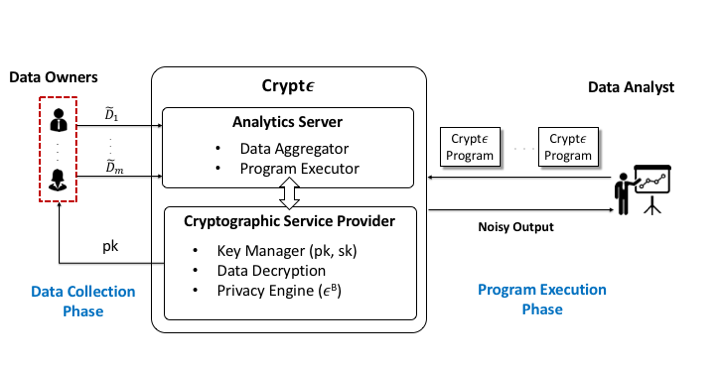
\includegraphics[width=\columnwidth]{diag.png}\caption{ Crypt$\epsilon$ System Setting: The  \textsf{AS} runs the Crypt$\epsilon$ programs. The \textsf{CSP} manages the cryptographic primitves. } \end{figure}
This section provides an overview of \system. We begin this section with the desiderata for \system that motivates our design followed by a discourse on the different components of \system and their functionality. Next we discuss about a few additional architectural choices we make for \system. This is followed by a description of \system's trust model and security sketch.

\subsection{Crypt$\epsilon$ Design}
The  desiderata for  the functionality of \system are as follows
\squishlist \item The architecture of \system should be able to support any differentially private algorithm that is permitted in the \textsf{CDP} model at the same order of accuracy guarantee as that of \textsf{CDP}, i.e. constant $O(\frac{1}{\epsilon})$ error bound.
\item Raw data records cannot be stored in the clear in any server, i.e., the server(s) in \system are untrusted. 
\item Data owners must be  off-line.\squishend
Recall from our discussion in section 1, \textsf{CDP} gives constant error bounds, however it relies on a trusted server for this. In contrast \textsf{LDP} requires no trusted server but results in limited accuracy.  The first two principles thus capture \system's objective of achieving the "best of both worlds", i.e., the accuracy guarantees and expressibility of the \textsf{CDP} model with  trust assumptions similar to that of the \textsf{LDP} model. The third principle stems from the fact that another undesirable trait of \textsf{LDP} is its inherent requirement for the data owners to be on-line during every query processing.  It is so because  in \textsf{LDP} %the private data of the individuals are not collated at a single place and hence%
depending on the query at hand, every time the data owners need to compute a different noisy measurement that best answers it. This is in general a poor practice as maintaining active communication channels for all the data owners might be unwieldy. \par The first desideratum can be achieved if we collate the data into a single data set such that any measurement can be performed on the entire data set at once followed by a single  instance of noise addition as opposed to aggregation over noisy measurements on individual data. The second desideratum mandates that the data hence collected should be suitably protected via cryptographic primitives (e.g. encryption scheme). Thus the first two requirements combined, necessitates \system to be able to perform differentially private computations on the encrypted data itself. This leads us to use linear homomorphic encryption and secure computation (specifically Yao's garbled circuits)  as the cryptographic primitives of our choice for \system. Note, by virtue of secure computation, we can potentially implement all the functionalities of the \textsf{CDP} model in \system. However, bearing the practical efficiency of the cryptographic primitives in mind, we impose certain limitations on the expressibility of \system. Due to the third desideratum, a generic $m+1$ party secure computation is ill-suited for our setting. This requires a third party entity that can factor out the onus of participating in a secure computation protocol from the data owners and capture its functionality in (at least) a 2-party protocol instead.   Moreover, since the data owners are no longer in the loop to monitor every query answering, the aforementioned entity should also watchdog the overall privacy budget expenditure. 
Guided by the above principles we design a two-server model for \system with the following components
\\(1)\textbf{ Data-Owners (\textsf{DO})} -  Each data-owner $\textsf{DO}_i, i \in [m]$ has  a
private data record $D_i$ and is willing to share it only if encrypted.   \\(2)\textbf{ Analytics Server (\textsf{AS})} - The \textsf{AS} wants to run a set of differentially private programs on the dataset $\mathcal{D}=\bigcup_{i=1}^m D_i$  but has 
access only to the encrypted copies of $D_i, i \in [m]$.
\\(3)\textbf{ Cryptographic Service Provider (\textsf{CSP})} -
 The \textsf{CSP} manages the cryptographic primitives used in Crypt$\epsilon$ and interacts with the \textsf{AS} to compute the
noisy answers. It is also responsible for monitoring the overall privacy budget expenditure.
%\xh{Rather than providing all the encryption details, can we just simply have an algorithm box to summarize the interactions between these three components. Then describe the interactions and highlight the key functionalities of each component, and then the trust model. }

 
 
\subsection{Crypt$\epsilon$ Modules}

\stitle{Cryptographic Service Provider (\textsf{CSP})}\\
(1)\textbf{ Key Manager }- The foremost duty of the \textsf{CSP} is to initialize the encryption scheme of Crypt$\epsilon$. This task is handled by the \textit{Key Manager} module which generates the key pair $(sk,pk)$ for the \textsf{labHE} scheme. It stores the secret key, $sk$ with itself and releases the public key, $pk$. Note that since the \textsf{CSP} has exclusive access to the secret key $sk$, it is the only entity capable of decryption in Crypt$\epsilon$.\\
(2)\textbf{ Data Decryption }- The \textsf{CSP} being the only entity capable of decryption,  any measurement of the data (even noisy) has to involve the \textsf{CSP}. The \textit{Data Decryption} module is tasked with handling all such interactions with the \textsf{AS}. \\
(3)\textbf{ Privacy Engine }- Crypt$\epsilon$ starts of with a total privacy budget of $\epsilon^B$ which is unanimously agreed upon by all the data owners. Note that the mechanism of deciding $\epsilon^B$ should be piloted by social prerogatives \cite{e1,e2} 
and is currently outside the scope of Crypt$\epsilon$. For executing any program, the \textsf{AS} has to interact with the \textsf{CSP} at least once (for decrypting the noisy answer) thereby giving the \textsf{CSP} the opportunity to monitor the \textsf{AS}'s actions in terms of privacy budget expenditure. The \textit{Privacy Engine} module hence maintains a public ledger that records the privacy budget spent in executing each program. Once the privacy cost incurred reaches 
$\epsilon^B$, the \textsf{CSP} refuses to decrypt any further answers thereby ensuring that the privacy budget is not exceeded.  The ledger is completely public allowing any data owner to verify it as and when desired.\\
\stitle{Data Owners (\textsf{DO})}\\
(1)\textbf{ Data Encoder} -  Each data owner $\textsf{DO}_i, i \in [m]$ has a private data record $D_i$ of the form $\langle A_1,...A_l\rangle$ where ${A}_j$ is an attribute. At the very outset, every data owner  $\textsf{DO}_i$ represents his/her private record $D_i$ in its respective per attribute one-hot-coding format. The one-hot-coding is a way of representation for categorical attributes and is illustrated by the following example. 
If the database schema in \system is given by  $\langle Age,Gender\rangle$ then corresponding one-hot-coding representation for a data owner $DO_i, i \in [m]$ with the record $\langle 30, Male\rangle$, is given by $\tilde{D_i}=\langle[\underbrace{0,\ldots,0}_{29},1,\underbrace{0,\ldots,0}_{70}],[1,0]\rangle$. \\
(2)\textbf{ Data Encryption} - The \textit{Data Encryption} module stores the public key $pk$ of the labHE scheme used in Crypt$\epsilon$ which is announced by the CSP. This key is used for an element-wise encryption of the data owner's  record of per attribute one-hot-codings. In our aforementioned example, we get $\mathbf{\tilde{D}}=\langle[\underbrace{labEnc_{pk}(0),\ldots}_{29},labEnc_{pk}(1),\\\underbrace{\ldots,labEnc_{pk}(0)}_{70}],
[labEnc_{pk}(1),labEnc_{pk}(0)]\rangle$. Finally the data owner sends this encrypted record to the \textsf{AS} via a secure channel. This is the only interaction that a data owner ever participates in, all the program executions are carried out by the \textsf{AS} and the \textsf{CSP} with the data owners being completely off line.\\
\stitle{Analytics Server (\textsf{AS)}}\\
(1)\textbf{  Aggregator} - The \textit{Aggregator} collects the encrypted records $\mathbf{\tilde{D_i}}$ from each of the data owners $\textsf{DO}_i$ and collates them into a single encrypted database $\boldsymbol{\tilde{\mathcal{D}}}$. %Note that in contrast, the server in the \textsf{CDP} model, being trusted, stores the data in the clear whereas in the \textsf{LDP} model the untrusted server stores appropriately randomized (noisy) data.   
\\(2)\textbf{ Program Executor }- The \textit{Program Executor} is the most important module of the \textsf{AS} and is tasked with the execution of Crypt$\epsilon$ programs. It takes as input a Crypt$\epsilon$ program from an external data analyst, alongside the appropriate privacy parameter $\epsilon$ and publishes the differentially private output computed with the assistance of the \textsf{CSP}. Crypt$\epsilon$ supports a set of 9 primitives and a Crypt$\epsilon$ program is an execution plan expressed as a sequence of these primitives. The primitives can be broadly classified into two types- transformation primitives and measurement primitives. Transformation primitives allow certain modifications on the encrypted data and are performed almost entirely by the \textsf{AS}. The measurement primitives on the other hand reveal some noisy measurement of the data and requires interaction with the \textsf{CSP}. \system supports two types of measurement primitives that implement two of the most popular differentially private mechanisms, Laplace mechanism \cite{Dork} and Noisy-Max \cite{Dork}. A typical Crypt$\epsilon$ program execution consists of  a series of transformation on the encrypted data followed by a measurement primitive and arbitrary post-processing. \\
 \textit{Noise Addition in \system} - For the Laplace mechanism, both the \textsf{AS} and the \textsf{CSP} add two separate instances of the random noise to the program output. This is necessary because had only one of them added the noise, then after the release of the clear text output, that party can simply subtract out the noise to reveal the true private answer. An alternative way can be both \AS and \CSP jointly computing a single instance of the noise using a secure computation protocol (see Appendix D.1). However, we do not implement it in the current version of \system as the two-fold noise addition is more efficient. For the Noisy-Max primitive, we provide an efficient secure computation protocol where only a single instance of noise by either party suffices. 
Since in Crypt$\epsilon$ the point of noise addition is just at the two servers, unlike at every individual in \textsf{LDP}, we achieve constant error bounds which is of the same order as that of \textsf{CDP} (see section \ref{exp:results}). 
\subsection{Crypt$\epsilon$ Workflow}
The complete workflow of Crypt$\epsilon$ is outlined as follows\\(1) \textbf{ Setup Phase} - This is the very first step in Crypt$\epsilon$ where the key manager of \textsf{CSP} generates the key pair for labHE $(sk,pk)$, publishes $pk$ and stores $sk$. \\(2) \textbf{ Data Collection Phase }- In the next phase, the $\textit{Data 
Encoder}$ and $\textit{Data Encryption}$ modules of every data owner, work to produce the encrypted data records which are then submitted to the \textsf{AS}. The data owners are relieved of all other duties and can go completely off-line. The $\textit{Aggregator}$ module of the \textsf{AS} then aggregates these encrypted records into a single encrypted database $\boldsymbol{\tilde{\mathcal{D}}}$. \\(3) \textbf{ Program Execution Phase} - In this phase, the \textsf{AS} executes a Crypt$\epsilon$ program with some interaction with the \textsf{CSP}  and generates a differentially private output.  \\
The \emph{Setup} and \emph{Data Collection} phases occur just once at the very beginning, every subsequent program  is handled via the corresponding  \emph{Program Execution} phase. Figure 1 shows the diagrammatic representation of \system. A comparative analysis of \system, \textsf{CDP} and \textsf{LDP} is presented in  Table \ref{DPCompare}.
\begin{table}[h!]
\centering
\caption {Comparative analysis of the different DP models \am{LDP does not have a data curator. Maybe a better way to put it is: Centralized Server: Yes/No. Trust assumption on Central Server: NA for LDP; Trusted for CDP and Untrusted/Non colluding for Crypte. Again Data storage in central server should be NA for LDP. Adversary should be Info.Theoretic for LDP and CDP and Computationally bounded for Crypte? Error should be Error on statistical counting query? I do not know about the impossibility result section. We need a tighter charaterization for CDP and Crypte. For instance, one can not learn a threshold function under CDP, but I would not call it unbounded sensitivity. I would drop the last line.  }}
\scalebox{0.6}{ \begin{tabular}{|l| c c c|}  \toprule
\multicolumn{1}{|c}{\textbf{Features}} & \textbf{LDP}  & \textbf{CDP}  & \textbf{Crypt$\epsilon$}  \\ [0.5ex] 
 \hline \hline\# Servers & 1& 1 & 2\\\hline
Trust  & & & Untrusted \\  Assumption & Untrusted & Trusted & Semi Honest \\for Server &  &   &  Non-Colluding  \\ \hline
Data Storage & \multirow{2}{*}{Noisy} & \multirow{2}{*}{Clear} & \multirow{2}{*}{Encrypted} \\in Server & &  &  \\\hline
Adversary & Unbounded & Unbounded & Bounded \\\hline
 Error & $O\Big(\frac{\sqrt(n)}{\epsilon}\Big)$& $O\Big(\frac{1}{\epsilon}\Big)$ & $O\Big(\frac{1}{\epsilon}\Big)$\\\hline
 Impossibility & Everything & Algorithms w/ & Same as that \\results & beyond SQ model & Unbounded Sensitivity & of \textsf{CDP} in theory \footnotemark\\
  [1ex] 
 \bottomrule
 \end{tabular}}\label{DPCompare}
\end{table}
\footnotetext{For practical constraints the current implementation has restrictions}
 %in between that of the central differential privacy model and the local differential privacy model - although it is definitely much weaker than that of the central differential privacy model, Crypt$\epsilon$'s trust model is slightly stronger as compared to that of the local differential privacy model owing to the aforementioned premises. 
%The formal security analysis for \system is presented in Appendix section B. 
\begin{comment}
learn any other information about the private datasets Di beyond what is revealed by the
model itself. Even in the case that one of the two servers (MLE or CSP) colludes with some
of the data-owners, they should learn no extra information about the data held by the
honest data-owners. In order to achieve this goal we design a system that can be seen as
multi-party protocol run by the m +2 parties mentioned before and specified by a sequence
of steps. This system (described in Section 4) has the following two-phase architecture:
We assume that the Evaluator and the CSP do not
collude. Each one may try to subvert the system as
discussed above, but they do so independently. More
precisely, at most one of these two parties is malicious:
this is an inherent requirement without which security
cannot be achieved.
• We assume that the setup works correctly, that is all
users obtain the correct public key from the CSP. This
can be enforced in practice with appropriate use of
Certificate Authorities.
Note that is true for any cryptographic primitive and is 
The can actually be avoided by removing the . m+1 secure computation where However this is Thus by capturing the we are having an huge efficincy gain now that teh problem is reduced to antwo-party

\subsection{Protocols} \xh{This might go first with the algorithm box or figure.}
In this section, for each of the three entities we list down the interactions that are initiated by them.
\begin{itemize}\item CSP- The foremost duty of the CSP is to initialize the encryption scheme of Crypt$\epsilon$. Specifically the CSP generates the key pair $(sk,pk)$ for the labeled homomorphic encryption. It stores $sk$ with itself and makes $pk$ public. Note that since only the CSP has access to the secret key $sk$, it is the only entity capable of decryption in Crypt$\epsilon$.
\item Data owners- Recall that each data owner owns a single private record which he/she shares with the AS in the encrypted form as follows. First every data owner represents his/her record in its respective per attribute one-hot-encoding format. For example, if the database schema is given by  $D=<Age,Gender>$ then a data owner with the record $<30, Male>$ would firstly represent it as $\mathcal{E}(D)=<[\underbrace{0,\ldots,0}_{29},1,\underbrace{0,\ldots,0}_{70}],[1,0]>$. This is followed by an element-wise encryption of this record of per attribute one-hot-encodings using the pubic key $pk$. In our aforementioned example, we get $\mathbf{D}=<[\underbrace{Enc(0),\ldots}_{29},Enc(1),\underbrace{\ldots,Enc(0)}_{70}],[Enc(1),Enc(0)]>$. Finally the data owner sends this encrypted record to the AS. Note that this is the only interaction that a data owner ever participates in. All the  query answering are carried out by the AS and the CSP with the data owners being completely off line. \item AS - After receiving the encrypted records from each of the data owners, the AS first collates them into a single encrypted database $\mathbf{\tilde{D}}$. For any subsequent query answering, $\mathbf{\tilde{D}}$ is subjected it to a series of transformations most of which are carried out by the AS by itself. However since the CSP is the only entity capable of decryption, for getting any measurement (even noisy) in the clear the AS has to interact with it. There are precisely two types of interactions between the AS and the CSP \begin{enumerate}\item Yao's Garbled Circuit \item Decryption of encrypted noisy value\end{enumerate}\end{itemize}
\end{comment}


\eat{Yet another alternative implementation could have been to engage the $m$ data owners and the \textsf{AS} in a $m+1$ secure computation protocol. This approach has two disadvantages. Firstly, as the number of data owners grow, the communication and computation overheads of this $m+1$ secure computation protocol would get prohibitively high. Secondly, this violates our requirement of off-line data owners. Thus by introducing a separate entity in the form of the \textsf{CSP}, we factor out the onus of participating in a secure multi party computation from the data owners and capture their computation power in a secure protocol between just the \textsf{CSP} and the \textsf{AS} instead %. Note that with the \textsf{CSP} in the picture, the secure computation is now reduced to a two-party case
irrespective of the number of data owners. %Not only does this improve the efficiency of our protocols drastically but is also advantageous from the perspective of ease of system implementation and maintenance. It is so because otherwise we would have had to maintain secure channels between all pairs of data owners, which would become extremely cumbersome with large values of $m$. Moreover all the data owners would have to be online for every program execution. Hence the choice of having a separate server in the form of the \textsf{CSP} is made from the efficiency point of view.
%The second assumption of an computationally bounded adversary is inherent in semantically secure cryptographic protocols. %Another design choice for Crypt$\epsilon$ could have been to keep the data owners in the loop for every program execution such that some of the data transformations could be pushed down to them. Since the data owners can perform the transformations on the plain text and in parallel, this could potentially improve performance. However this would require the data owners to be on-line during the program execution which might be unwieldy in practice especially with a large number of geographically dispersed data owners. 
\par %Keeping the efficiency of our implementation in mind, we used only two instances of simple two-party Yao's garbled circuits for Crypt$\epsilon$. In addition, we propose two optimizations that leverage on the fact that the \textsf{AS} is satisfied with differentially private outputs; this allows  us to expend some of the privacy budget in differentially private pre-processing of the encrypted data. 
The class of programs supported by Crypt$\epsilon$ is any program that can be expressed as a composition of  Crypt$\epsilon$ primitives followed by arbitrary post-processing. Crypt$\epsilon$ supports 7 transformation primitives and 2 measurement primitives. The noisy measurements allowed are the Laplace mechanism and the Noisy max (see section 4.2), two of the most popular and standard differentially private algorithms. The main constraint behind the design of the transformation primitives is that their composition should allow seamless sensitivity analysis.  Sensitivity analysis of arbitrary relational algebraic queries is a hard problem, for e.g. sensitivity of conjunctive counting queries with join operator is unbounded \cite{sensitivity}. Hence all the transformations that Crypt$\epsilon$ supports have bounded stability \cite{PINQ} such that the sensitivity analysis of any program written using them is straightforward. In fact, we showcase that the proposed Crypt$\epsilon$ primitives are indeed very powerful, enabling us to answer practically useful queries, such as linear counting queries etc. 
\\ 
}





\subsection{Trust Model}
Both the servers, \textsf{AS} and \textsf{CSP} are completely untrusted in Crypt$\epsilon$. 
Thus from the data owners perspective the trust assumption is similar to that of \textsf{LDP}; the data owners need not place their trust in any external entity. 
However there are two modest differences in the Crypt$\epsilon$ setting from that of \textsf{LDP}.\\
 (1) We assume that the \textsf{AS} and the \textsf{CSP} are non-colluding and follow the \emph{honest-but-curious} (or \textit{semi-honest}) adversary model. %That is, they always follow the instructions of the protocol faithfully but strive to learn extra information about the private records from the messages received during the execution of the protocol. 
 Moreover we assume that each data owner has a private channel with the \textsf{AS}. This is to prevent any third party (including the \textsf{CSP}) from eavesdropping. \\
 (2) The adversary is now reduced to a \textit{computationally bounded} one as opposed to the information theoretic one  in \textsf{LDP}.
 

 \subsection{\system Security Sketch}
 Let $\Pi$ represent the protocol for the end-to-end execution of a $\epsilon$-DP program in \system.  In this paper we consider a
semi-honest adversary  $Adv$ (see section 3.4) who can corrupt any subset of the data owners, the data analyst and at most one of the two
servers. This captures our assumption that the two servers are non-colluding. Thus the requisite security definition should state that $Adv$ only learns the data of the corrupted data owners and the differentially private output but nothing else about the honest data owners. In other words, the view of the adversary $Adv$ should be \emph{computationally indistinguishable} from a truly differentially private protocol. 
Let $P$ be a program that is submitted by the data analyst to the protocol $\Pi$ and it is to be run on the data set $\mathcal{D}$ with the privacy parameter $\epsilon$. Thus based on our discussion on noise addition in sec 3.2, we define the ideal functionality $\mathcal{F}=(\mathcal{F}_1,\mathcal{F}_2)$ of the protocol $\Pi$ as follows.
\\If $P$ uses Laplace mechanism \cite{Dork}, then
\begin{gather} 
\mathcal{F}_1(P,\mathcal{D},\epsilon)=P(\mathcal{D})+\eta_2\\\mathcal{F}_2(P,\mathcal{D},\epsilon)=P(\mathcal{D})+\eta_1 \\ \eta_1, \eta_2 \sim Lap(\frac{\Delta}{\epsilon})\end{gather}  where  $\Delta$  is the suitable sensitivity of the program. In this case, $output^{\Pi}(P,\mathcal{D})$ which denotes the published output of \system, is given by $P(\mathcal{D})+\eta_1+\eta_2$.\\
If $P$ uses Noisy-Max mechanism \cite{Dork}, then
\begin{multline}
\mathcal{F}_1(P,\mathcal{D},\epsilon)=\mathcal{F}_2(P,\mathcal{D},\epsilon)=Noisy-Max(P(\mathcal{D}),\Delta,\epsilon) 
\end{multline} where $P(\mathcal{D})$ produces a vector and  $\Delta$ is the suitable sensitivity of the program. $output^{\Pi}(P,\mathcal{D},)$ in this case is equal to $Noisy-Max(P(\mathcal{D}),\Delta,\epsilon)$.\\
Formally, using the standard simulation based definition \cite{Oded},
\begin{theorem}  Let $S \subset \{1,...,m\}$ then $\Pi$, (i.e. the protocol for an end-to-end program execution in \system) realizes $\mathcal{F}$ (eq 3-6)  with correctness and privacy against
the adversaries $Adv_1=\textsf{AS} \cup \{\textsf{DO}_i, i \in S\} \cup \mbox{Data Analyst}$  and $Adv_2=\textsf{CSP} \cup  \{ \textsf{DO}_i, i \in S\} \cup \mbox{Data Analyst}$
 if there exists  P.P.T algorithms $Sim_1$ and $Sim_2$ such that  \begin{align*}
 \big\{Sim_1({D_i, i \in S},\mathcal{F}_1(P,\mathcal{D},\epsilon)),\mathcal{F}(P,\mathcal{D},\epsilon)\big\} &\\\stackrel{C}{\equiv} \big\{view^{\Pi}_{Adv1}(P,\mathcal{D}),output^{\Pi}(P,\mathcal{D})\big\}  \numberthis\label{adv1}
               \\
 \big\{Sim_2({D_i, i \in S},\mathcal{F}_2(P,\mathcal{D},\epsilon)),\mathcal{F}(P,\mathcal{D},\epsilon))\big\} &\\\stackrel{C}{\equiv}\big\{ view^{\Pi}_{Adv2}(P,\mathcal{D}),output^{\Pi}(P,\mathcal{D})\big\}  \numberthis\label{adv2}
\end{align*} for all possible inputs  where $ \stackrel{C}{\equiv}$ denotes computational indistinguishability and $view^{\Pi}_i$ denotes the view of entity $i$ in protocol $\Pi$. 
\end{theorem}
\begin{corollary} Protocol $\Pi$ satisfies \textsf{SIM-CDP} \cite{CDP} privacy.\end{corollary}
The proof of this is presented in Appendix A. \eat{Here we just present an intuitive understanding of it. The interactions between the \textsf{AS} and the \textsf{CSP} can be categorised as \\(1) \textsf{CSP} generates garbled circuits with noisy outputs that are evaluated by the \textsf{AS}\\(2) \textsf{AS} sends encrypted masked data to the \textsf{CSP} and gets a transformed encrypted data in response \\(3)\textsf{AS} sends encrypted noisy data and gets back the data in the cleat with additional noise from the \textsf{CSP}\\
The garbled circuits are inherently semantically secure. For the second type of interaction, the random
mask hides the true plaintext
from the \textsf{CSP} while the \textsf{AS} cannot decrypt anything as it does not have access to the secret key $sk$. The last type of interaction outputs a noisy measurement over the data and illustrates the fact that both  \textsf{AS} and \textsf{CSP} add noise to the final answer in \system to ensure that both the servers are allowed only a differentially private  view of the data. Moreover, in
addition to the \emph{Program Executor} module of the \textsf{AS}, the data analyst
communicates the \system program and the privacy parameter $\epsilon$
to the \textit{Privacy Engine} module of the \textsf{CSP}. This enables the \textsf{CSP} to
compute the sensitivity of the program for itself (required while
adding its own noise) thereby thwarting any privacy budget over
expenditure attempts.}
 




\subsection{Discussion on Crypt$\epsilon$ architecture}\label{architecture}
 Crypt$\epsilon$  is based on the premise that there are $m$  data owners, each possessing a private data record, and the \textsf{AS} is the primary entity who is interested in learning certain differentially private statistics on the collective data.  Thus in \system, we require the \textsf{AS} to  shoulder the major chunk of the workload for any Crypt$\epsilon$ program execution; interactions with the \textsf{CSP} should be minimal and only related to data decryption.
Keeping this in  mind, we design the \textsf{AS} to perform most of the data transformations by itself (Table \ref{perf}). Specifically for every Crypt$\epsilon$ program, the \textsf{AS} processes the whole database and transforms it into concise representations (like an encrypted scalar or a short vector) which is then decrypted with the help of the \textsf{CSP}. It is interesting to note that we could have had an alternative implementation for Crypt$\epsilon$ where the private database is equally shared between the two servers and they engage in a secret share based secure computation protocol for computing the differentially private answers. However, this would require both the servers to do almost equal amount of work for every program. Such an arrangement would be justified only if both the servers are equally invested in learning the differentially private statistics and is ill-suited for Crypt$\epsilon$. Additionally, a secret-share based computation would be much more communication intensive resulting in a performance hit. 

The primitives for \system have been designed bearing two things in mind. Firstly, their composition should allow easy sensitivity analysis (for e.g. transformations must have bounded stability). Secondly, all the primitives should have very efficient implementations. Thus although the architecture of \system imposes no fundamental restriction on its expressibility and in theory we can enjoy the same algorithmic power as that of \textsf{CDP}, we restrict the expressibility in the current implementation of \system to ensure practicality of \system programs. Nevertheless, there is a separation between \system and \textsf{LDP} as explained in Appendix D2.


\eat{\begin{table}[h!]
\small
\centering
\caption {Comparative analysis of the different DP models}
 \begin{tabular}{l| c c c}  \toprule
\multicolumn{1}{c}{\textbf{Features}} & \textbf{LDP}  & \textbf{CDP}  & \textbf{Crypt$\epsilon$}  \\ [0.5ex] 
 \midrule \midrule \# Servers & 1& 1 & 2\\\hline
Trust  & & & Untrusted \\  Assumption & Untrusted & Trusted & Semi Honest \\for Server &  &   &  Non-Colluding  \\ \hline
Data Storage & \multirow{2}{*}{Noisy} & \multirow{2}{*}{Clear} & \multirow{2}{*}{Encrypted} \\in Server & &  &  \\\hline
Adversary & Unbounded & Unbounded & Bounded \\\hline
 Error & $O\Big(\frac{\sqrt(n)}{\epsilon}\Big)$& $O\Big(\frac{1}{\epsilon}\Big)$ & $O\Big(\frac{1}{\epsilon}\Big)$\\\hline
 Impossibility & Everything && \\results & beyond SQ model & None & None\footnotemark\\
  [1ex] 
 \bottomrule
 \end{tabular}
\end{table}
\footnotetext{Theoretically no restriction, however practical constraints maybe present}}

%\arc{ Can add another column for Mixnets maybe?}

%!TEX root = main.tex

\section{\system Primitives}\label{sec:primitives}

Given a database schema $\langle A_1,\ldots,A_k \rangle$ and an encrypted instance of this database, $\encD$, \system permits data analysts to author \textit{logical} \system programs on $\encD$ with differential privacy guarantee.  The logical programs mainly consist of data transformation operators inspired by relational algebra and differentially private measurement operators. These programs can  have constructs like looping and conditionals, and can arbitrarily post-process outputs of measurement operators. \system compiles these logical programs into \system protocols that can work on the encrypted data on the \textsf{AS} and \textsf{CSP}. Though these logical \system programs are designed to run on encrypted data, when operating them on plaintext data, they give differential privacy under \textsf{CDP}.
%\am{Should we say that logical \system program when operating on the raw data gives you DP under CDP? }

In this section, we define the primitives for data transformations and differentially private measures (summarized in Table~\ref{tab:primitives}). Then, we illustrate how to write logical programs using these primitives to express state-of-the art DP algorithms under the \cdp model. In Section~\ref{sec:implementation} we describe how \system compiles these down to protocols that work on encrypted data.

% Please add the following required packages to your document preamble:
% \usepackage{multirow}


\begin{table*}[]
\small{
\caption {\system Primitives}\label{tab:primitives}
\begin{tabular}{|l|l|l|l|l|l|}
\hline
\bf{Types}                           & \bf{Name}         & \bf{Notation} & \bf{Input} & \bf{Output} & \bf{Functionality} \\ \hline \hline
\multirow{7}{*}{Transformation} & \multirow{2}{*}{\textsf{CrossProduct}} &  \multirow{2}{*}{$\crossproduct_{A_i,A_j\rightarrow A'}(\cdot)$} & 

\multirow{2}{*}{$\encT$}   &  \multirow{2}{*}{$\encT'$}   & Generates a new attribute  $A'$ (in one-hot-coding) to represent\\ & & & & & the data for both the attributes $A_i$ and $A_j$   \\ \cline{2-6}
                                & \textsf{Project}     & $\project_{A^*}(\cdot)$  &  $\encT$       &  $\encT'$       &  Discards all attributes but $A*$ \\ \cline{2-6}
                                & \textsf{Filter}       & $\filter_{\phi}(\cdot)$   &  $\encT$      &   $\encB'$     &  Zeros out records not satisfying $\phi$    in $\encB$          \\ \cline{2-6}
                                & \textsf{Count}             & $\countagg(\cdot)$         & $\encT$  &  $\encC$    &  Counts the number of 1s in $\encB$               \\ \cline{2-6}
                                & \textsf{GroupByCount*}             & $\groupbystar_{A}(\cdot)$ &  $\encT$  & $\encV$    & Returns encrypted histogram of $A$                \\ \cline{2-6}
                                & \textsf{GroupByCount}              & $\groupbystar_{A}(\cdot)$    &$\encT$       & $\tilde{\encV}$        &  Returns encrypted histogram of $A$ in one-hot-encoding    \\ \cline{2-6}
                                & \textsf{CountDistinct}             & $\countdistinct(\cdot)$     &    $\encV$   & $\encC$   &  Counts the number of non-zero values in $\encV$       \\ \hline
\multirow{2}{*}{Measurement}    & \textsf{Laplace}     & $\lap_{\epsilon,\Delta}(\cdot)$    &  $\encV$      &   $\hat{V}$    &  Adds Laplace noise to $\encV$    \\ \cline{2-6}
                                & \textsf{NoisyMax}     & $\noisymax_{\epsilon,\Delta}^k(\cdot)$         & $\encV$       &  $\hat{\mathcal{P}}$      &  %Adds Laplace noise to $\encV$ and 
                                Returns indices of the top $k$ noisy values              \\ \hline
\end{tabular}
}
\end{table*}


\eat{
\begin{table*}[h!]
\small
\caption {\system Primitives}
 \begin{tabular}{@{}l c@{}c@{}l@{}}  \toprule
\multicolumn{1}{c}{\textbf{Primitives}} & \textbf{Input}  & \textbf{Output}  & \multicolumn{1}{c}{\textbf{Functionality}}  \\ [0.5ex] 
 \midrule \midrule \textsf{CrossProduct} &$\tilde{\mathbf{T}}, A_i, A_j$ & $\tilde{\mathbf{T'}}$ & Generates  one-hot-coding for the\\&& & attribute $A_i\times A_j$ 
 \\\textsf{Project}&$\tilde{\mathbf{T}}, A^*$&$\tilde{\mathbf{T'}}$ &Discards all attributes but $A^*$
 \\\textsf{Filter}&$\tilde{\mathbf{T}},\phi$&$\tilde{\mathbf{B}}$&Zeros out records not satisfying $\phi$
 \\\textsf{Count}&$\tilde{\mathbf{T}}$&$\mathbf{C}$&Counts the number of records in $\textbf{B}$ 
 \\$\textsf{GroupBy}^*$ &$\tilde{\mathbf{T}},A$&$\mathbf{V}$& Returns encrypted histogram of $A$
 \\\textsf{GroupBy} &$\tilde{\mathbf{T}},A$ &$\tilde{\mathbf{V}}$ &Returns encrypted histogram of $A$\\&&& in one-hot-coding
 \\\textsf{CountDistinct} &$\mathbf{V}$&$\mathbf{C}$ &Counts the number of non-zero values in $\textbf{V}$
 \\\textsf{Laplace}&$\textbf{V},\epsilon$ &$\hat{\textbf{V}}$ & Both \textsf{CSP} and {AS} adds Laplace noise to $\textbf{V}$ 
 \\\textsf{NoisyMax} & $\textbf{V},\epsilon, k$&$P$ &Outputs top k values from noisy vector $\textbf{V}$\\
  [1ex] 
 \bottomrule
 \end{tabular}
\end{table*}
}


\subsection{Transformation Primitives}\label{sec:transformation_primitives}
Transformation primitives take an encrypted data as input and output a transformed encrypted data.  These primitives thus work completely on the encrypted data and do not expend any privacy budget. Three types of data are considered in this context: (1) an encrypted table of $x$ rows and $y$ columns/attributes, denoted by $\encT$, where each attribute value is represented by encrypted one-hot-encoding of the value; (2) an encrypted vector of numbers, denoted by $\encV$; and (3) an encrypted scalar, denoted by $\encC$. In addition, every encrypted table $\encT$ of $x$ rows has a encrypted bit vector $\encB$ of size $x$ to indicate whether the record is relevant to the program at hand. If the $i$-th bit value of $B$ is $1$, then the $i$-th row in $\encT$ will be used for answering the current program and vice versa. The input to the very first transformation primitive in \system program is the encrypted database $\encD$ with all bits of $\encB$ set to be $1$. For brevity, we just use $\encT$ to represent both the encrypted table $\encT$ and $\encB$. The transformation primitives are detailed below.

\stitle{{\normalfont(1)} \textsf{CrossProduct}} $\crossproduct_{(A_i,A_j)\rightarrow A'}(\encT)$: This primitive transforms the two encrypted one-hot-encodings for attributes $A_i$ and $A_j$ in $\encT$ into a single encrypted one-hot-encoding of a new attribute $A'$. The domain of the new attribute $A'$ is the cross product of the domains for $A_i$ and $A_j$. The resulting table $\encT'$ has one column less than $\encT$. Thus, the construction of the one-hot-coding of the entire $y$-dimensional domain can be computed by repeated application of this primitive. 	
%1) \textbf{\textsf{CrossProduct}}:$\crossproduct_{A_1,A_2}(\tilde{\mathbf{T}})$ - Given encrypted one-hot-codings for two different attributes $A_1$ and $A_2$ of domain sizes $s_{A_1}$ and $s_{A_2}$ respectively, the goal of this transformation is to compute the encrypted one-hot-coding for the entire two-dimension domain of the new $\lq$attribute' $A_1\times A_2$ of size $s_{A_1}\cdot s_{A_2}$. Thus this transformation takes as input a $x \times y $ table, $\tilde{\mathbf{T}}$ defined over attribute set $A=\{A_1,A_2,...,A_y\}$ where each cell $\tilde{\mathbf{T}}[i,j] , i \in [x], j \in [y], 2 \leq y \leq k$ corresponds to the encrypted one-hot-coding for attribute $A_j$ for the data owner $\textsf{DO}_i$ and outputs a $x \times (y-1)$ table with attribute set $\{A_1\times A_2,A_3,\ldots,A_{y}\}$.  Note that the construction of the one-hot-coding of the full $y$-dimension domain can be computed by repeated application of this transform. 	

\stitle{{\normalfont(2)} \textsf{Project}} $\project_{\bar{A}}(\encT)$: This primitive projects $\encT$ on  a subset of attributes $\bar{A}$ of the input table. All the attributes that are not in $\bar{A}$ are discarded from the output table $\encT'$.
	%2) \textbf{\textsf{Project}} : $\project_{A^*}(\tilde{\mathbf{T}})$- In addition to the $ x \times y$ table, $\tilde{\mathbf{T}}$ over attribute set $\{A_1, A_2, ..., A_y\}$, the \textsf{Project} transformation takes a set of attributes $A*=\{A^*_1,...A^*_p\}, p < y$ as inputs. The result of the transformation is defined as the $x \times p$ data source table where each record is just restricted to the attribute set $A^*$, i.e., it discards all other attributes. 
	%Infact it is analogous to the operation of marginalization which is described as follows.
	%Assuming  $A$ and $B$ to be two attributes with finite domains, let $x$ be a vector of counts representing a histogram over the cross product of the domain (with $|A|*|B|$ entries).
	%Marginalization over the attribute $B$ results in a vector of counts on the attribute $A$ alone by adding up counts corresponding to the same value of $A$.  


\stitle{{\normalfont(3)} \textsf{Filter}} $\filter_{\phi}(\encT)$: This primitive specifies a filtering condition, represented by a boolean predicate $\phi$ defined over a subset of attributes $\bar{A}$ of the input table $\encT$. The predicate can be expressed as a conjunction of range conditions over $\bar{A}$, i.e. for a row $r \in [x]$ in $\encT$, $\phi(r) = \bigwedge_{A_i \in \bar{A}} ~~(r.{A_i} \in V_{A_i})$,  where $r.A_i$ is value of attribute $A_i$ in row $r$ and $V_A$ is a subset of values (can be a singleton too) that attribute $A_i$ can take.  For example, $Age\in [30,40]\wedge Gender=M$ can be one such  filtering condition. The \textsf{Filter} primitive affects only the associated encrypted bit vector of $\encT$ and keeps the actual table untouched.  In this primitive, if any row $r \in [x]$ in $\encT$ does not satisfy the filtering condition $\phi$, the corresponding $r^{th}$ bit in $\encB$ will be set to $labEnc_{pk}(0)$; otherwise, the corresponding bit value in $\encB$ is kept unchanged.  Thus the \textsf{Filter} transformation suppresses all the records that are extraneous to answering the program at hand (i.e., does not satisfy $\phi$) by explicitly zeroing the corresponding indicator bits and outputs the table $\encT'$ with the updated indicator vector.


\stitle{{\normalfont(4)} \textsf{Count}} $\countagg(\encT)$: This primitive simply counts the number of rows in $\encT$ that are pertinent to the program at hand, i.e. the number of $1$s in its associated bit vector $\encB$.  This primitive outputs an encrypted scalar $\encC$. 
%Typically, this transformation is followed by a measurement primitive and is immediately preceded by a \textsf{Filter} primitive. \\
% 4) \textbf{\textsf{Count}}$:\countagg(\mathbf{T})$  - The \textsf{Count} transformation outputs the encrypted value of the non-noisy true count for the program at hand. For answering linear counting queries, typically \textsf{Count}  is the last transformation to be applied and is immediately preceded by a \textsf{Filter} transformation. Recall that the \textsf{Filter} transformation sets bit $i \in [m]$ to be 1 (encrypted) if the $i^{th}$ record satisfies the filter condition and 0 otherwise and outputs this encrypted $m\times 1$ vector. Hence the \textsf{Count} primitive simply adds up all the entries of this bit vector $\mathbf{B}$ and  outputs the sum which is a single encrypted value. 

\stitle{{\normalfont(5)} \textsf{GroupByCount*}} $\groupbystar_{A}(\mathbf{\tilde{T}})$: The  \textsf{GroupByCount*} primitive buckets the input table $\mathbf{\tilde{T}}$ into groups of records having the same value for an attribute $A$. The output of this transformation is thus, an encrypted  vector $\mathbf{V}$ which is the encrypted histogram for $A$.    This primitive serves as a preceding transformation for other Crypt$\epsilon$ primitives such as \textsf{NoisyMax}, \textsf{CountDistinct}.

\stitle{{\normalfont(6)} \textsf{GroupByCount}} $\groupby_{A}(\mathbf{\tilde{T}})$ : This primitive is similar to the aforementioned \textsf{GroupByCount*} primitive. The only difference between the two is that, \textsf{GroupByCount} outputs the encrypted histogram of attribute $A$ with each count represented in one-hot-coding, $\tilde{V}$.  This transformation allows us to answer queries based on the count of a particular value for attribute $A$.

\stitle{{\normalfont(7)} \textsf{CountDistinct } }$\countdistinct(\mathbf{V})$: As mentioned above, this primitive is always preceded by a \textsf{GroupByCount*} primitive. Hence the input vector $\mathbf{V}$ is an encrypted histogram for some attribute $A$ and this primitive returns the number of distinct values of $A$ that appear in  $\boldsymbol{\tilde{\mathcal{D}}}$ by counting the non-zero entries of $V$.
%The input to Crypt$\epsilon$ is an encrypted instance of a database $\boldsymbol{\tilde{\mathcal{D}}}$ with a single relational schema $\langle \mathcal{A}_1,\mathcal{A}_2, . . . ,\mathcal{A}_l\rangle$. Each attribute $\mathcal{A}_i$ is assumed to be discrete (or suitably discretized) and represented in one-hot-coding form.



\eat{
Transformation primitives take as input an encrypted source variable (a table of size $x \times y, x,y \in \mathcal{Z}_{\geq 0}$) and output a transformed data source (again  a table $x' \times y', x',y' \in \mathcal{Z}_{\geq 0}$) that is still encrypted. Typically $x$ and $x'$ are equal to $m$, the total number of data owners, i.e., every tuple in the data source tables corresponds to the record of a single data owner. In case $x=1$ or $x'=1$ the data source is an encrypted vector and we represent it as $\mathbf{V}$.
The transformation primitives are mostly carried out by the \textsf{AS} on its own; this is enabled by our use of labeled homomorphic encryption scheme which allows us to perform certain operations, specifically multiplication and addition, directly over the encrypted data. %Only two transformations  (\textsf{GroupBy} and \textsf{CountDistinct}) need to be computed via a secure computation protocol between the \textsf{AS} and the \textsf{CSP}. 
Since these primitives work entirely on encrypted data, they do not expend the privacy budget. However these operators can affect the privacy analysis through their stability. Every transformation in Crypt$\epsilon$ has a well-established stability.
For each record of the database $\boldsymbol{\tilde{\mathcal{D}}}$ (i.e., data corresponding to a single data owner) we maintain an encrypted bit which indicates whether the record is relevant to the program at hand. Let $\mathbf{B}$ represent this bit vector where $\mathbf{B}[i]$ corresponds to this indicator bit for the $i^{th}$ record.  If $\mathbf{B}[i] =Enc_{pk}(1)$, then the $i^{th}$ record is to be considered for answering the current program and vice versa. Only one of the transformation, \textsf{Filter} alters the bit vector $\mathbf{B}$. Before every program execution, $\mathbf{B}$ is initialized to a 1-vector. 
\begin{enumerate}

	\item \textsf{CrossProduct} ($\tilde{\mathbf{T}}, A_i, A_j$) - Given encrypted one-hot-codings for two different attributes $A_1$ and $A_2$ of domain sizes $s_{A_1}$ and $s_{A_2}$ respectively, the goal of this transformation is to compute the encrypted one-hot-coding for the entire two-dimension domain of the new $\lq$attribute' $A_1\times A_2$ of size $s_{A_1}\cdot s_{A_2}$. Thus this transformation takes as input a $x \times y $ table, $\tilde{\mathbf{T}}$ defined over attribute set $A=\{A_1,A_2,...,A_y\}$ where each cell $\tilde{\mathbf{T}}[i,j] , i \in [x], j \in [y], 2 \leq y \leq k$ corresponds to the encrypted one-hot-coding for attribute $A_j$ for the data owner $\textsf{DO}_i$ and outputs a $x \times (y-1)$ table with attribute set $\{A_1\times A_2,A_3,\ldots,A_{y}\}$.  Note that the construction of the one-hot-coding of the full $y$-dimension domain can be computed by repeated application of this transform. 	
    
	
	\item \textsf{Project}($\tilde{\mathbf{T}},A^*$)- In addition to the $ x \times y$ table, $\tilde{\mathbf{T}}$ over attribute set $\{A_1, A_2, ..., A_y\}$, the \textsf{Project} transformation takes a set of attributes $A*=\{A^*_1,...A^*_p\}, p < y$ as inputs. The result of the transformation is defined as the $x \times p$ data source table where each record is just restricted to the attribute set $A^*$, i.e., it discards all other attributes. \\
	%Infact it is analogous to the operation of marginalization which is described as follows.
	%Assuming  $A$ and $B$ to be two attributes with finite domains, let $x$ be a vector of counts representing a histogram over the cross product of the domain (with $|A|*|B|$ entries).
	%Marginalization over the attribute $B$ results in a vector of counts on the attribute $A$ alone by adding up counts corresponding to the same value of $A$.  
  \item \textsf{Filter}($\tilde{\mathbf{T}},\phi$) - Let $\tilde{\mathbf{T}}$ be an encrypted table of one-hot-codings over attribute set $A=\{A_1,...,A_k\}$, $\phi$ be a  predicate defined over a subset of attributes $A^*\subseteq A$ and $\mathbf{B}$ be the current state of the indicator vector which is stored by the \textsf{AS}. The predicate $\phi$ has to be expressed as a conjunction of range conditions over $A^*$, i.e.,\begin{gather}\phi = \bigwedge_{A \in A^*}(A \in \{v_{1},\ldots,v_{t}\} ) \label{phi} \end{gather} If for some attribute $A \in A^*$, the condition is a equality condition as $A==v$ instead of a range condition, then simply put $v_1=v_t$. For e.g., a condition of this form is find the number of records that satisfy $Age$ in range [30,40] and $Gender$ is male. For each record $r_i, i \in [m]$, the Filter transformation zeros the corresponding indicator bit $\mathbf{B}[i] $ if $\phi(r_i)=False$. $\mathbf{B}[i] $ is kept unchanged otherwise. Thus the \textsf{Filter} transformation suppresses all the records that are extraneous to answering the program at hand (i.e., does not satisfy $\phi$) by explicitly zeroing the corresponding indicator bits and outputs the updated indicator vector. %It takes as input a $x \times 1$ table $\tilde{\mathbf{T}}$, whose every row is an encrypted one-hot-encoding (of the form $\mathbf{\tilde{R}}$) for the attribute of concern $A$, and a vector $\mathbf{C}$ which has encryptions of appropriate non-zero weights for indices that satisfy $\phi$. %Note that $A$ need not be an attribute of the original attribute set $\mathcal{A}$ but can be a new multi-dimension 'attribute' constructed over $\mathcal{A}^* \subseteq \mathcal{A}$, i.e., $A= \prod_{A*_i \in \mathcal{A}^*  }A^*_i$. 
    \item{\textsf{Count}($\mathbf{T}$) } - The \textsf{Count} transformation outputs the encrypted value of the non-noisy true count for the program at hand. For answering linear counting queries, typically \textsf{Count}  is the last transformation to be applied and is immediately preceded by a \textsf{Filter} transformation. Recall that the \textsf{Filter} transformation sets bit $i \in [m]$ to be 1 (encrypted) if the $i^{th}$ record satisfies the filter condition and 0 otherwise and outputs this encrypted $m\times 1$ vector. Hence the \textsf{Count} primitive simply adds up all the entries of this bit vector $\mathbf{B}$ and  outputs the sum which is a single encrypted value. 
    \item{\textsf{GroupBy*}($\mathbf{\tilde{T}},A$)}- The purpose of the \textsf{GroupBy*} transformation is to essentially bucket the input $x\times y$ table $\mathbf{\tilde{T}}$ into groups of records having the same value for an attribute of choice $A$. The output of this transformation is an $1\times s_A$ encrypted  vector $\mathbf{V}$  where each vector element $\mathbf{V}[i], i \in [s_A]$ represents the encrypted count of the number of records in $\boldsymbol{\tilde{\mathcal{D}}}$ having value $v_{i}$ for attribute $A$. Thus \textsf{GroupBy*} essentially returns an encrypted histogram for $A$.
    This primitive serves as a preceding transformation for other Crypt$\epsilon$ primitives like \textsf{NoisyMax}, \textsf{CountDistinct} et al.
     \item{\textsf{GroupBy}($\mathbf{\tilde{T}},A$)-} The \textsf{GroupBy} transformation is similar to the aforementioned \textsf{GroupBy*} transformation. The only difference between the two is that, the former outputs the encrypted one-hot-coding of the respective counts. That is, the output of \textsf{GroupBy}($A$)  is an $s_A$ lengthed encrypted vector $\tilde{\mathbf{V}}$ such that each element, $\tilde{\mathbf{V}}[i], i \in [s_A]$ represents the encrypted one-hot-encoding of the number of records in $\boldsymbol{\tilde{\mathcal{D}}}$ having value $v_{i}$ for attribuet $A$. This transformation allows us to answer queries based on the count of a particular value for attribute $A$.
     %Note that since for \textsf{GroupBy} we need to create the one-hot-coding of the counts, this requires an interaction with the \textsf{CSP}.
     \item {\textsf{CountDistinct}($\mathbf{V}$)-} As mentioned before, the \textsf{CountDistinct} primitive takes as input an encrypted vector $\mathbf{V}$ which is the output of a \textsf{GroupBy*}($A$) primitive for some attribute $A$. Thus the \textsf{CountDistinct} primitive  returns the number of distinct values of $A$ that appear in the records of $\boldsymbol{\tilde{\mathcal{D}}}$ by counting the non-zero entries of $V$.  
\end{enumerate}
%Note that the first four transformations namely \textsf{CrossProduct, Project, Filter} and Count are performed by the \textsf{AS} alone. Only for transformation \textsf{GroupBy} the \textsf{AS} engages in a secure computation protocol with the \textsf{CSP}.

}%%%ENDOF EAT


\subsection{Measurement Primitives} \label{sec:measurement_primitives}
The measurement primitives take encrypted vector of counts $\encV$ (or a single count $\encC$) as input and return noisy measurements on it in the clear. These two primitives correspond to two classic differentially private mechanisms: Laplace mechanism and Noisy-Max mechanism~\cite{Dork}. Both mechanisms add noise $\eta$ drawn from Laplace distribution, denoted by $Lap(b)$, where $\Pr[\eta =x]\propto e^{-{\frac{|x|}{b}}}$. The scale of the noise depends on the transformations applied on the base database $\mathcal{D}$. 

Let the sequence of transformations ($\bar{\mathcal{T}}=(\mathcal{T}_l,\ldots,\mathcal{T}_1)$) applied on $\encD$ to get $V$ be $\bar{\mathcal{T}}(D) = \mathcal{T}_l(\cdots \mathcal{T}_2((\mathcal{T}_1(D))))$. We define the \emph{sensitivity} of a sequence of transformations as  the maximum change to the output of this sequence of transformations when changing a row in the input database, i.e., $\Delta_{\bar{\mathcal{T}}} = \max_{D,D'} \|\bar{\mathcal{T}}(D)-\bar{\mathcal{T}}(D')\|_1$ where $D$ and $D'$ differ but a single record. The sensitivity of $\bar{\mathcal{T}}$ can be upper bounded by the product of the stability (Theorem~\ref{theorem:stability}) of these transformation primitives, i.e. $\Delta_{\bar{\mathcal{T}}=(\mathcal{T}_l,\ldots,\mathcal{T}_1)} = \prod_{i=1}^l \Delta \mathcal{T}_i$. The transformation operators in Table~\ref{tab:primitives} have a stability of 1, except for \textsf{GroupByCount} and \textsf{GroupByCount*} which are 2-stable. Given $\epsilon$ and $\Delta_{\bar{\mathcal{T}}}$, we define the two measurement primitives as follows.


\stitle{{\normalfont(1)} \textsf{Laplace}} $\lap_{\epsilon,\Delta}(\mathbf{V}/\encC)$:  This primitive implements the classic Laplace mechanism \cite{Dork}. Given an encrypted vector $\encV$ or an encrypted scalar $\encC$, a privacy parameter $\epsilon$ and sensitivity $\Delta$ of the preceding transformations, the primitive adds a noise vector (scalar) from $Lap(\frac{\Delta}{\epsilon})$. This primitive ensures $\epsilon$-differential privacy when data analyst views the plaintext answer.

\stitle{{\normalfont(2)} \textsf{NoisyMax }} $\noisymax_{\epsilon,\Delta}^k(\mathbf{V})$:  Noisy-Max is a type of differentially private selection mechanism \cite{Dork} where the goal is to determine the query with the highest value out of $n$ different noisy query outputs. The algorithm works as follows. First, generate each of the $n$ answers and then add independent Laplace noise from the distribution $Lap(\frac{\Delta}{\epsilon})$ to each of them. The indices of the top-k noisy values, $\hat{\mathcal{P}}$ are then reported as the desired answer. 

\eat{
Thus they expend the privacy budget and require secure computation between the \textsf{AS} and the \textsf{CSP}. 
\begin{comment} All measurement operators must involve joint computation with the \textsf{CSP}. Note that the requisite noise to be added to ensure differentially privacy has to be jointly added by both the \textsf{AS} and the \textsf{CSP}. It is so because, had only either one of the servers added the noise, then that server would be able to retrieve the true non-noisy answer by simply de-noising the published differentially private answer. This means that the sensitivity of the program being executed should be known to both the servers. This poses no hindrance in our setting  since the program is public, the  sensitivity computation can be performed very easily by observing the sequence of the preceding transformations.
\end{comment}
\begin{enumerate}
	\item \textsf{Laplace}($\mathbf{V},\epsilon$) - In the Laplace mechanism, in order
to publish $f(D)$ where $f : D \mapsto R$, $\epsilon$-differentially private mechanism $\mathcal{M()}$ 
publishes $f(D) + Lap\Big(\frac{\Delta f}{\epsilon}\Big)$  
where $\Delta f = \max_{D,D'}||f(D)-f(D')||_1$ is known as the sensitivity of the query. The p.d.f of $Lap(b)$ is given by\begin{gather}\mathbf{f}(x)={\frac  {1}{2b}}e^{ \left(-{\frac  {|x-\mu |}{b}}\right)}\end{gather} The sensitivity of the function $f$ basically captures the magnitude by which a single individual's data can change the function $f$ in the worst case. Therefore, intuitively, it captures the uncertainty in the response that we must introduce in order to hide the participation of a single individual. For counting queries the sensitivity is 1. The \textsf{Laplace} primitive enables the \textsf{AS} and the \textsf{CSP} to add two separate instances of random laplace noise to the true result of a counting query for generating a differentially private output. It takes an input an encrypted vector $\mathbf{V}$ (could be a scalar too) and adds two instances of noise drawn from $[Lap(\frac{1}{\epsilon})]^{|V|}$ to it.

	\item \textsf{NoisyMax}($\mathbf{V},\epsilon, k$)-Noisy-Max is a type of differentially-private selection mechanism where the goal is to determine the counting query with the highest value out of $n$ different counts.  
	The algorithm works as follows. First, generate each of the counts and then add independent Laplace noise from the distribution $Lap(\frac{1}{\epsilon})$ to each of them. The index of the largest noisy count is then reported as the noisy max.
	This has two fold advantage over the naive implementation of finding the maximum count.
Firstly, noisy-max applies "information minimization" as rather than releasing all the noisy counts
and allowing the analyst to find the max and its index, only the
index corresponding to the maximum is made public.
Secondly, the noise added is much smaller than that in the case of the naive implementation (it has sensitivity $\Delta f=m$). Thus the \textsf{NoisyMax} primitive takes as input of encrypted vector where each vector element is a count. It then adds noise drawn from $Lap(\frac{1}{\epsilon})$ to each vector element and computes the indices of the top k elements.
\end{enumerate}
}

\subsection{Program Examples}
Consider a database scheme ($Age$, $Gender$, $NativeCountry$, $Department$, $Salary$). We will show several \system program examples in Table~\ref{tab:programexamples}.
\begin{table*}[t]
\caption{Examples for \system Program}\label{tab:programexamples}
\scalebox{0.75}{
\begin{tabular}{|l|l|}
\hline
 {\bf Program} & {\bf Answer} \\ \hline \hline
P1:  $\lap_{\epsilon,1}(\countagg(\filter_{Age\in [50,60]}(\project_{Age}(\encD))))$ &  the number of records satisfying $Age \in [50,60]$      \\ \hline
P2: $\noisymax^5_{\epsilon,1}(\groupbystar_{Age}(\encD))$               &       the 5 most frequent age values \\ \hline
P3: $\lap_{\epsilon,1}(\groupbystar_{Age\times Gender}(\project_{Age \times Gender}(\crossproduct_{Age,Gender}(\encD))))$     &       the marginal over attributes Age and Gender values \\ \hline
P4: $\lap_{\epsilon,1}(\groupbystar_{Age\times Gender}(\filter_{NativeCountry=Mexico}(\project_{Age\times Gender, NativeCountry}(\crossproduct_{Age,Gender}(\encD)))))$                          & the marginal over Age and Gender where NativeCountry is Mexico       \\ \hline
P5: $\lap_{\epsilon,1}(\countagg(\filter_{Age=30 \wedge Gender=Male \wedge NativeCountry=Mexico}(\project_{Age,Gender,NtiveCountry}(\encD))))$,                                       &    the number of for male employees of US having age =50    \\ \hline
P6:   $\lap_{\epsilon,1}(\countdistinct(\groupbystar_{Age}(\filter_{Gender=Male}(\project_{Age \times Gender}(\encD)))))$ & the number of distinct age values for the male employees in the database       \\ \hline
P7:  $\lap_{\epsilon,1}(\countagg(\filter_{Count\in[10,m]}(\groupby_{Age}(\project_{Age}(\encD)))))$
                                     &    the number of  age values having at least 10 records in the database    \\ \hline
\end{tabular}}
\end{table*}


\section{Implementation}\label{sec:implementation}
%To demonstrate the use of Crypt$\epsilon$ primitives let us look at the following example.
\label{implementation}
In this section we describe the implementation of \system. First we discuss our proposed technique for extending the $labMult$ operation of \textsf{labHE} to support $n > 2$ multiplicands. Then we describe the implementations of \system primitive. Last, we present a  classification of the \system programs. 
\begin{algorithm}[b]
\caption{$genLabMult$ - generate label for $labMult$}\label{algo:genlabmult}
\small
\begin{algorithmic}[1]
\STATEx
\textbf{Input}: $\mathbf{c_1}=(a_1,d_1)=labEnc_{pk}(m_1)$ and $\mathbf{c_2}=labEnc_{pk}(m_2)$ 
\STATEx where $a_1= m_1-b_1, d_1=Enc_{pk}(b_1)$, $a_2= m_2-b_2, d_2=Enc_{pk}(b_2)$
\STATEx \textbf{Output}: $\mathbf{e}=labEnc_{pk}(m_1\cdot m_2)$
\STATEx \textbf{\textsf{AS}:} 
\STATE Computes $\textbf{e}'=labMult(\mathbf{c_1,c_2}) \oplus Enc_{pk}(r)$ where $r$ is a random mask 
\STATEx  //$e'$ corresponds to $m_1\cdot m_2-b_1\cdot b_2+r$
\STATE Sends $\mathbf{e'},d_1,d_2$ to \textsf{CSP}
\STATEx \textbf{\textsf{CSP}:}
\STATE Computes $e''= Dec_{sk}(\mathbf{e'}) + Dec_{sk}(d_1)\cdot Dec_{sk}(d_2)$
\STATEx //$e''$ corresponds to $m_1\cdot m_2 + r$ 
%\STATE Decrypts $\mathbf{e'}$, to get $Dec_{sk}(\mathbf{e}')=m_1\cdot m_2 -b_2\cdot b_1 + r$
%\STATE Computes $b_1 \cdot b_2$ from $d_1$ and $d_2$.
%\STATE Removes $b_1\cdot b_2$ from $e'$ to compute $e''=m_1\cdot m_2+r$
\STATE Picks a seed $\sigma'$ and label $\tau'$ and computes $b'=\mathcal{F}(\sigma',\tau')$ 
%\STATE Computes $\bar{a}=e''-b'=m_1\cdot m_2 +r -b'$,  and $d'=Enc_{pk}(b')$
\STATE Sends $\bar{e}=(\bar{a},d')$ to \textsf{AS}, where $\bar{a} = e''-b'$ and $d' = Enc_{pk}(b')$
\STATEx //$\bar{a}$ corresponds to $m_1\cdot m_2 + r-b'$.
\STATEx \textbf{\textsf{AS}:}
\STATE Computes true cipher $\mathbf{e}=(a',d')$ where $a'=\bar{a}-r$ %m_1\cdot m_2 - b'$
 \end{algorithmic}
\end{algorithm}


\subsection{\textbf{General $n$-way Multiplication for \textsf{labHE}}}\label{genlab}
In addition to the operations supported by an \textsf{LHE}  scheme, \textsf{labHE} supports multiplication of two \textsf{labHE} ciphers. 
\squishlist
\item $\textbf{labMult}(\mathbf{c}_1,\mathbf{c}_2)$ - On input two \textsf{labHE} ciphers $\mathbf{c}_1=(a_1,d_1)$ and $\mathbf{c}_2=(a_2,d_2)$, it computes a "multiplication" ciphertext  $\mathbf{e}=labMult(\mathbf{c_1,}$ $\mathbf{c_2})=Enc_{pk}(a_1,a_2)\oplus cMult(d_1,a_2) \oplus cMult(d_2,a_1)$. Observe that $Dec_{sk}(\mathbf{e})=m_1\cdot m_2 -b_1 \cdot b_2$.
\item $\textbf{labMultDec}_{sk}(d_1,d_2,\mathbf{e})$ - On input two encrypted masks $d_1,d_2$ of two \textsf{labHE} ciphers $\mathbf{c_1},\mathbf{c_2}$, this algorithm decryts the output $\mathbf{e}$ of $labMult(\mathbf{c_1},\mathbf{c_2})$ as $m_3=Dec_{sk}(\mathbf{e})+Dec_{sk}(d_1)\cdot Dec_{sk}(d_2)$ which is equals to $m_1\cdot m_2$.   
\squishend
However, these algorithms cannot be used directly for a $n$-way muplication where $n>2$.  It is so because the "multiplication" cipher $\mathbf{e}=labMult(\mathbf{c_1},\mathbf{c_2})$ does not have  a corresponding label, i.e., it is not in the correct \textsf{labHE} cipher representation. Hence we propose Algorithm~\ref{algo:genlabmult} to generate a label $\tau'$ and a seed $b'$ for every intermediary product of two multiplicands so that it we can do a generic $n$-way multiplication on the ciphers. Note that the mask $r$ protects the value of $(m_1\cdot m_2)$ from the \textsf{CSP} (Step 3) and $b'$ hides $(m_1\cdot m_2)$ from the \textsf{AS} (Step 6). 
For example, suppose we want to multiply the respective ciphers of  $4$ messages $\{m_1,m_2,m_3,m_4\} \in \mathcal{M}^4$ and obtain $\mathbf{e}=labEnc_{pk}(m_1\cdot m_2\cdot m_3 \cdot m_4)$. For this, the \textsf{AS} first generates $\mathbf{e_{1,2}}=labEnc_{pk}(m_1\cdot m_2)$ and $\mathbf{e_{3,4}}=labEnc_{pk}(m_3\cdot m_4)$ using Algorithm~\ref{algo:genlabmult}. Both operations can be done in parallel in just one interaction round between the \textsf{AS} and the \textsf{CSP}. In the next round,  the \textsf{AS} can again use Algorithm~\ref{algo:genlabmult} with inputs $\mathbf{e_{1,2}}$ and $\mathbf{e_{3,4}}$ to obtain the final answer $\mathbf{e}$. %consider a case of mu Now with the true \textsf{labHE} cipher $\mathbf{c}=(a',d')$ for the product the \textsf{AS} can compute further multiplications on it. 
Thus for a generic $n-way$ multiplication the order of multiplication can be, in fact, parallelized as  shown in Figure ~\ref{genlab-fig} (Appendix) to require a total of $\lceil \log n\rceil$ rounds of communication with the \textsf{CSP}.

%In this paper we propose an efficient way of extending the $labMult$ operation for a $n$-way multiplication. Let's consider an example case where we want to multiply the respective ciphers of  $4$ messages $\{m_1,m_2,m_3,m_4\} \in \mathcal{M}^4$ and obtain $\mathbf{e}=labEnc_{pk}(m_1\cdot m_2\cdot m_3 \cdot m_4)$. Note that the reason why we can't directly use  $labMult$ for a $4-$ way multiplication is because, the "multiplication" cipher $\mathbf{e}=labMult(\mathbf{c_1},\mathbf{c_2})$ does not have  a corresponding label, i.e., it is not in the correct \textsf{labHE} cipher representation. Thus for generalizing the $labMult$ operation for $n>2$ multiplicands what we have to do is to generate a label and a seed for every intermediary product of two multiplicands. This can be done as shown by Algorithm 1. Note that the mask $r$ protects the value of $m_1\cdot m_2$ from the \textsf{CSP} in step 5. Similarly since $b'$ is not known to the \textsf{AS}, $m_1\cdot m_2$ remains hidden from the \textsf{AS} in step 9.
 

\subsection{Primitive Implementation}
%Now let us explain the implementation details of the aforementioned Crypt$\epsilon$ primitives.  
Here we explain the implementation details of two of the  \system primitives. The rest are covered in Appendix~\ref{app:implement_primitives}.

\stitle{\textsf{GroupByCount }} $\groupbystar_A(\mathbf{\tilde{T}})$: The implemenation of this primitive is summarized in Algorithm~\ref{groupby-imp}. First, the \textsf{AS} uses the $\textsf{GroupByCount}^*$ primitive to generate the encrypted histogram $\encV$ for attribute $A$. Since each entry of $\mathbf{V}$ is a count of records, its value ranges from $\{0,...,m\}$. The \textsf{AS} then masks $\encV$ (step 2) and sends it to the \textsf{CSP}. The purpose of this mask is to hide the true histogram from the \textsf{CSP}. Next the \textsf{CSP} generates the encrypted one-hot-coding representation for this masked histogram $\boldsymbol{\tilde{\mathcal{V}}}$ (steps 4-5) and returns it back to the \textsf{AS}. %Notice that each entry of $\boldsymbol{\tilde{\mathcal{V}}}$ is a $m$-length vector. 
The \textsf{AS} can simply rotate $\boldsymbol{\tilde{\mathcal{V}}}[i], i \in [|V|]$ by its respective mask value $M[i]$ (step 7) and get back the true encrypted histogram in one-hot-coding $\tilde{\encV}$.
Note that the \textsf{GroupByCount} primitive could have an alternative implementation using a garbled circuit that takes as input the encrypted vector and outputs the corresponding one-hot-coding representation. However this would require the circuit to decrypt and re-encrypt $O(m)$ data inside it which would be very costly. 
 


\begin{algorithm}[t]
\small{
\caption{\textsf{GroupByCount }$\tilde{\encV} \leftarrow \groupby_A(\mathbf{\tilde{T}})$}
\begin{algorithmic}[1]
%\STATEx \textbf{Input}: $\mathbf{\tilde{T}}$
%\STATEx \textbf{Output}:
\STATEx \textbf{\textsf{AS}:} \STATE Computes $\mathbf{V}=\groupbystar_{A}(\encT)$.
\STATE Masks the encrypted histogram $\mathbf{V}$ for attribute $A$ as follows 
$$\boldsymbol{\mathcal{V}}[i]= \mathbf{V}[i] \oplus labEnc_{pk}(M[i]), ~~~~\text{where, }M[i] \in_R [m], i \in [|V|]$$
\STATE Sends $\boldsymbol{\mathcal{V}}$ to \textsf{CSP}.
\STATEx \textbf{\textsf{CSP}:}
\STATE Decrypts  $\boldsymbol{\mathcal{V}}$ as $\mathcal{V}[i]=labDec_{sk}(\boldsymbol{\mathcal{V}}), i \in [|V|]$.\STATE Converts each entry of $\mathcal{V}$ to its corresponding one-hot-coding and encrypts it, $\boldsymbol{\tilde{\mathcal{V}}}[i]=labEnc_{pk}(\tilde{\mathcal{V}[i]}), i \in [|V|]$
\STATE Sends $\boldsymbol{\tilde{\mathcal{V}}}$ to \textsf{AS}.
\STATEx \textbf{\textsf{AS}}:
\STATE  Rotates every entry by its corresponding mask value to obtain the desired  encrypted one-hot-coding $\boldsymbol{\tilde{V}}[i]$. \begin{gather*}\boldsymbol{\tilde{V}}[i]=RightRotate(\boldsymbol{\tilde{\mathcal{V}}},M[i]), i \in [|V|]\end{gather*} 
 \end{algorithmic} \label{groupby-imp}}
\end{algorithm} 


\stitle{\textsf{Laplace }}$\lap_{\epsilon,\Delta}(\mathbf{V})$:  Recall that both \textsf{AS} and \textsf{CSP} have to add Laplace noise to the output in Crypt$\epsilon$. Hence the \textsf{Laplace} primitive  has two phases. In the first phase,  the \textsf{AS} adds an instance of encrypted Laplace noise $\eta_1 \sim Lap(\frac{\Delta}{\epsilon})$ to the encrypted input \eat{(step 1 in Algorithm ~\ref{lap})} to generate $\mathbf{\hat{\mathcal{V}}}$. This acts as the input to the second phase which is executed by the \textsf{CSP}. Here the \textsf{CSP} decrypts $\mathbf{\hat{\mathcal{V}}}$ and adds a second instance of the Laplace noise $\eta_2 \sim Lap(\frac{\Delta}{\epsilon})$ to generate the final noisy output $\hat{V}$ in the clear. %(steps 3-4)
The \textsf{Laplace} primitive with an encrypted scalar $\encC$ as the input is implemented in a similar way.
 %Another observation is that this double noise addition does not affect the differential privacy guarantee. After the addition of the first instance of noise by the \textsf{AS}, the second can be seen as a post-processing step. Hence our results Crypt$\epsilon$ programs are still differentially private by Theorem 2.
%\textit{Note:} Following our discussion on the primitive implementations in this section and Appendix C, we see that the major chunk of the work for almost all the transformation primitives is carried out the \textsf{AS} by itself. This conforms to our second requirement in section.



\eat{\begin{algorithm}
\small{
\caption{\textsf{Laplace }$\lap_{\epsilon,\Delta}(\mathbf{V})$}
\begin{algorithmic}[1]
\STATEx
\textbf{Input}: $\encV$
\STATEx \textbf{Output}: $\hat{V}$
\STATEx \textbf{\textsf{AS}:} \STATE Generates a noisy vector $\hat{\encV}$  as \begin{gather*}\hat{\mathbf{V}}[i] = \mathbf{V}[i]\oplus labEnc_{pk}(\eta[i]),\\ \eta \sim [Lap(\frac{1}{\epsilon})]^{|V|}, i \in [|V|] \end{gather*}
\STATE Sends $\hat{\mathbb{\mathcal{V}}}$  to \textsf{CSP}
\STATEx \textbf{\textsf{CSP}:}
\STATE Decrypts $\mathbf{\hat{\mathcal{V}}}$ to get $\hat{\mathcal{V}}[i]=labDec_{sk}(\mathbf{\hat{\mathcal{V}}}[i]), i \in [|V|]$
\STATE Generates a the final noisy vector $\hat{V}$ as follows 
\begin{gather*} \hat{V}[i]=\hat{\mathcal{V}}[i]+\eta'[i], i \in [|V|], \eta' \sim [Lap(\frac{1}{\epsilon})]^{|\hat{V}|} \end{gather*}
\STATE Returns $\hat{V}$ to \textsf{AS}
 \end{algorithmic} \label{lap}
}
\end{algorithm}} %The implementation for the \textsf{Laplace} primitive is given by Algorithm ~\ref{lap}.

\subsection{Classification of \system Programs}
\system programs can be grouped into three classes based on the number and type of interaction between the \textsf{AS} and the \textsf{CSP}. 

\stitle{Class I : Single Decrypt Interaction Programs}\\
Recall that the transformation primitives output encrypted data.  Since  the \textsf{CSP} has exclusive access to the secret key, it is the only party in \system capable of decryption. Thus for releasing any result (albeit noisy) in the clear, the \textsf{AS} needs to interact at least once with the \textsf{CSP}. \system supports this type of interactions via the two measurement primitives. Some \system programs require only a single interaction of this type at the very end to release the noisy output. All other transformations can be performed by the \textsf{AS} via homomorphic operations on the encrypted data records. Typically these programs filter the database on a single attribute. Examples of this type of programs are P1, P2 and P3 from Table~\ref{tab:programexamples}.

\stitle{Class II : \textsf{LabHE} Multiplication Interaction Programs}\\
Recall that \textsf{labHE} allows multiplication of two ciphers. \system can support a general $n$-way multiplcation of ciphers for $n > 2$ as described in Section~\ref{genlab}. However it requires intermediate interactions with the \textsf{CSP}. Thus all \system programs that require multiplication of more than two ciphers need interaction with the \textsf{CSP}.  All programs that filter the database on more than three attributes would thus fall under this class. P4 and P5 from Table~\ref{tab:programexamples} are in this class.

\stitle{Class III : Other Interaction Programs}\\
 The \textsf{GroupBy} primitive requires an intermediate interaction with the \textsf{CSP} (for generating the encrypted one-hot-coding). The \textsf{CountDistinct} primitive also uses a garbled circuit (Appendix~\ref{app:implement_primitives}) and hence requires interactions with the \textsf{CSP}. This is in addition to the interaction required for decrypting the noisy answer (as explained in Class I above). Therefore, any program with the \textsf{GroupBy} or \textsf{CountDistinct} primitive requires at least two rounds of interaction. P6 and P7 from Table~\ref{tab:programexamples} are examples of this class of \system programs. 


\eat{
\begin{frame}{}
  \begin{center}
    \scalebox{0.75}{
    \begin{minipage}{1\linewidth}
\begin{algorithm}[H]
\caption{\textsf{GroupByCount }$\groupby_A(\mathbf{\tilde{T}})$}
\begin{algorithmic}[1]
\STATEx
\textbf{Input}: $\mathbf{\tilde{T}}$
\STATEx \textbf{Output}: $\tilde{\encV}$
\STATEx \textbf{\textsf{AS}:} \STATE Computes $\mathbf{V}=\groupbystar_{A}(\encT)$.
\STATE Masks the encrypted histogram $\mathbf{V}$ for attribute $A$ as follows \begin{gather*}\boldsymbol{\mathcal{V}}[i]= \mathbf{V}[i] \oplus labEnc_{pk}(M[i])\\M[i] \in_R [m], i \in [|V|]\end{gather*}
\STATE Sends $\boldsymbol{\mathcal{V}}$ to \textsf{CSP}.
\STATEx \textbf{\textsf{CSP}:}
\STATE Decrypts  $\boldsymbol{\mathcal{V}}$ as $\mathcal{V}[i]=labDec_{sk}(\boldsymbol{\mathcal{V}}), i \in [|V|]$.\STATE Converts each entry of $\mathcal{V}$ to its corresponding one-hot-coding and encrypts it, $\boldsymbol{\tilde{\mathcal{V}}}[i]=labEnc_{pk}(\tilde{\mathcal{V}[i]}), i \in [|V|]$
\STATE Sends $\boldsymbol{\tilde{\mathcal{V}}}$ to \textsf{AS}.
\STATEx \textbf{\textsf{AS}}:
\STATE  Rotates every entry by its corresponding mask value to obtain the desired  encrypted one-hot-coding $\boldsymbol{\tilde{V}}[i]$. \begin{gather*}\boldsymbol{\tilde{V}}[i]=RightRotate(\boldsymbol{\tilde{\mathcal{V}}},M[i]), i \in [|V|]\end{gather*} 
 \end{algorithmic} \label{groupby-imp}
\end{algorithm} 
 \end{minipage}}
  \end{center}
\end{frame}
}

\section{\system Optimizations}\label{sec:optimization}
In this section we present several optimization techniques used by \system. These optimizations do not alter the end-to-end privacy guarantees of the system. 

\subsection{Novel \system Differential Privacy Based Optimization}\label{sec:dp_optimization}
This optimization expend some of the overall $\epsilon$ privacy budget to build differentially private indexes that can be used to speed up computation on encrypted data.


\stitle{{\normalfont (1)} DP Indexing}: This optimization is motivated by the fact that several programs first filter out a large fraction of the rows in the dataset. For instance, the program  P5 in Table~\ref{tab:programexamples} constructs a histogram over $Age$ and $Gender$ on the subset of data for which $NativeCountry$ is Mexico. Our filter implementation keeps all the rows (even if they do not satisfy the condition) as the \textsf{AS} has no way to tell if the filter condition is satisfied or not. This results in the subsequent GroupbyCount* being run on the full data instead of on a small subset. If there were an index on $NativeCountry$,  \system could run the GroupbyCount* on only the subset of records that have $NativeCountry$=Mexico instead of on the entire dataset, but an exact index would leak the true data distribution, violating DP. 

Hence, \system allows a differentially private index be built on a prespecified attribute $A$ on the encrypted database $\encD$.   Let $P=(P_1,\ldots,P_k)$ be a uniform partition on the sorted domain of $A$ such that each partition contains $\frac{s_A}{k}$ consecutive domain values. First we use a garbled circuit to sort $\encD$ over $A$ into $\encD_s$ and additionally output a noisy cumulative histogram $\hat{V}$ on this $k$ partitions, $\hat{V}[i]=\sum_j ct_{A,j}+\eta_i$ where $i \in [k], j \in \cup_{l=1}^i P_k, \eta_i\sim Lap(k/\epsilon_A)$ and $ct_{A,j}$ denotes the number of records with value $j$ for attribute $A$. 
Next the \textsf{AS} computes a noisy c.d.f, $\hat{\mathcal{C}}$ over the $k$ bins using the noisy counts in $\hat{V}$ using inference based on isotonic regression \cite{cdf}. For executing a program conditioned as $\phi=A \in [v_s,v_e]$, we compute first compute $i_{start}=\hat{\mathcal{C}}[r_s-1], v_s \in [\frac{s_A}{k}\cdot(r_s-1)+1,\frac{s_A}{k}\cdot r_s]$, i.e., $v_s$ belongs to bin $r_s$   and  $i_{end}=\hat{\mathcal{C}}[r_e], v_e \in [\frac{s_A}{k}\cdot(r_e-1)+1,\frac{s_A}{k}\cdot r_e]$, i.e., $v_e$ belongs to bin $r_e$. We then run the program on this subset of records in $[i_{start},i_{end}]$. For increased accuracy we can also consider preceding bins of $r_s-1$ for $i_{start}$ and succeeding bins of $r_e$ for $i_{end}$.

There are two heuristics that can be considered for selecting the indexing attribute $A$. First, $A$ should be very frequently queried. This is intuitive as this would mean a larger fraction of the queries will benefit from this optimization. Second, if $\{v_1,...v_n\} \subset dom(A)$ is the set of most frequently queried values for attribute $A$, then $ct_{A,i}, i \in [n] << m$ where $ct_{A,i}$ is the number of records in $\encD$ having value $v_i$ for attribute $A$. This would ensure that the first selection performed alone on $A$ will filter out majority of the records and reduce the intermediate dataset size to be considered for the subsequent predicate.

%\xh{May move the following to appendix} This circuit takes (i) the secret key $sk$ from the \CPS, and (ii) the entire database $\encD$ and the attribute $A$ from the \AS. The attribute $A$ has a domain of size $s_A$ and is uniformly partitioned into $k$ ranges $\{R_1,\ldots, R_i, \ldots, R_{s_A/k}\}$, where $R_i = [\frac{s_A}{k}i, \frac{s_A}{k}(i+1))$.  This circuit first decrypts $\encD$ using the secret key and sorts the decrypted database on attribute $A$ in ascending order. The sorted database is then encrypted again. Then the circuit computes a histogram $V$ on the $k$ ranges of $A$, denoted by $[c_1,\ldots,c_k]$  and perturbs each count with Laplace noise, i.e., $\hat{c}_i = c_i + \eta_i$, where $\eta_i\sim Lap(1/\epsilon)$. 
%Then the \AS use the noisy counts $\encV$ to construct a cumulative histogram over $A$, where $\hat{cdf}[i] = \sum_{j=0}^i \hat{c}_i$ and post-processed such that they are in non-decreasing order and non-negative, and $\hat{cdf}[k] = |\encD|$~\cite{cdf}.  Given the differentially private cumulative histogram as the index and the sorted database, when a program would like to select rows with $A\in [v_i, v_j]$, we find the ranges that contain $v_i$ and $v_j$ respectively, denoted by $R_i$ and $R_j$. Then we return all records in the sorted database which cover all ranges from $R_i$ and $R_j$. This corresponds to row $(\hat{cdf}[i-1]+1)$ to row $(\hat{cdf}[j])$.

\eat{
Given an encrypted database $\encD$ and an attribute $A$ of $\encD$, we first use a garbled circuit to sort $\encD$ over $A$ into $\encD_s$ and then build a differentially private indexing on the sorted database $\encD_s$ (details in Appendix B.2). Next we build the index on $A$ with a privacy budget $\epsilon_{A}$ as follows. Let $P=(P_1,\ldots,P_k)$ be a uniform partition on the sorted domain of $A$ such that each partition contains $\frac{s_A}{k}$ consecutive domain values. We compute a noisy CDF $\hat{\mathcal{C}}$ vector $\hat{V}$ of length $k$ such that $\hat{V}[i]=\sum_j ct_{A,j}+\eta_i$ where $i \in [k], j \in P_i$ and $\eta_i\sim Lap(1/\epsilon_A)$. 
Next the \textsf{AS} computes a noisy CDF, $\hat{\mathcal{C}}$ over the $k$ bins using the noisy counts in $\hat{V}$ using inference based on isotonic regression \cite{cdf}. For executing a program conditioned as $\phi=A \in [v_s,v_e]$, we compute first compute $i_{start}=\hat{\mathcal{C}}[r_s-1], v_s \in [\frac{s_A}{k}\cdot(r_s-1)+1,\frac{s_A}{k}\cdot r_s]$, i.e., $v_s$ belongs to bin $r_s$   and  $i_{end}=\hat{\mathcal{C}}[r_e], v_e \in [\frac{s_A}{k}\cdot(r_e-1)+1,\frac{s_A}{k}\cdot r_e]$, i.e., $v_e$ belongs to bin $r_e$. We then run the program on this subset of records in $[i_{start},i_{end}]$. For increased accuracy we can also consider preceding bins of $r_s-1$ for $i_{start}$ and succeeding bins of $r_e$ for $i_{end}$.
}

\squishlist
\item \textbf{Optimized feature} - This optimization speeds up the execution time by reducing the number of total records to be processed for the program execution.
\item \textbf{Trade-off} - The trade-off is  a possible increase in error as the noisy selection of records from the index might miss some of the records that do satisfy the filter condition.
\item \textbf{Privacy Cost} - Assuming the index is constructed with a privacy parameter $\epsilon_A$, a selection of a subset of records using it will result in a $\epsilon_A$ - DP intermediate result. If $\epsilon$ is the parameter used for the subsequent measurement primitives, then by Theorem 1, the total privacy parameter is $\epsilon_A+\epsilon$.
\squishend



\begin{comment}
For answering queries of the form $\phi=A_1==v_1\wedge \ldots  \wedge A_n==v_n$, ideally we just need to compute for $A_2==v_2\wedge \ldots \wedge A_n==v_n$ on $ct_{A,v}$ number of records starting from position $\sum_{i=1}^{i=v-1}ct_{A,i}$ of $\boldsymbol{\mathcal{\tilde{D}}}_{sort}$. 

However the \textsf{AS} has access only to the noisy CDF over the $k$ bins $ct_{A,i}$. Note that when $\bar{i}_{start}=\bar{\hat{\mathcal{C}}}[v-1] < \sum_{i=1}^{i=v-1}ct_{A,i}$ and $\bar{i}_{end}= \bar{\hat{\mathcal{C}}}[v-1] > i_{start}+ct_{A,v}$, i.e., the indices computed from the noisy values  saddle over the true records satisfying $A==v$, then although we end up loosing in performance a bit, we are still guaranteed to compute the exact non-noisy count for records satisfying $\phi$. 

In all other cases, we end up disregarding some of the records that satisfy $A==v$, some of these rejected records in fact might additionally satisfy $A_1==v_1 \wedge \ldots \wedge A_n==v_n$. Thus we might get inaccurate answer for query predicate $\phi$ (note that here we are talking about the encrypted true count of the given query predicate that is computed by the AS via a series of transformations before applying the LaplaceMechanism primitive).  An effective heuristic to tackle this can be to compensate for the expected laplacian error as follows  $\bar{i}_{start}= \bar{\hat{\mathcal{C}}}[v-1]-\frac{2}{\epsilon}$ and $\bar{i}_{end}=\bar{\hat{\mathcal{C}}}[v]+\frac{2}{\epsilon}$. Also note that answering differentially private  range queries   on attribute $A$ can also be directly done from the noisy CDF $\bar{\hat{\mathcal{C}}}$ 
\end{comment}



 


\subsection{Crypto-Engineering Optimizations} \label{sec:im_optimization}
In this section we present three crypto-engineering optimizations. The first one (DP range tree) expends privacy budget and but results in better accuracy in the long run. The other two optimizations (precomputation and off-line processing) work completely on the encrypted data and do not expend any privacy budget. Hence they do not affect the accuracy of the executed programs.


\stitle{{\normalfont (1)} DP Range Tree}:
Range queries constitute a very popular category of queries for typical databases and range trees are a popular data structure constructed to speed up range query answering. 
A 1-dimensional range tree for an attribute $A$ is an ordered hierarchical data structure such that the leaf nodes correspond to the individual counts for each possible value of $A$, while the parent nodes cover a range of values and store the sum of the counts of its children. Hence, if range queries are common, pre-computing noisy range trees is an useful optimization, e.g. building a range tree on $Age$ attribute can be useful for programs P1 and P2 in Table~\ref{tab:programexamples}. The sensitivity for  such a noisy range tree is $\log s_A$ where $s_A$ is the domain size of the attribute on which the tree is constructed. To answer any arbitrary range query, we need to access at most $2\log s_A$ number of nodes in the range tree. Thus to answer all possible range queries on $A$, the total squared error accumulated is $O(\frac{s^2(\log s_A)^2 }{\epsilon})$. In contrast for the naive case, we would have incurred error $O(\frac{s_A^3}{\epsilon})$ \cite{cdf}. Hence this range tree optimization not only gives us a huge performance boost but also results in better answer accuracy.


%A 1-dimensional range tree for an attribute $A$ is an ordered data structure such that the leaf nodes correspond to the individual counts $ct_{A,i}$, $v_i \in dom(A)$ while each parent node stores the sum of the counts of its children. Hence an useful optimization for \system can be pre-computing the noisy range tree for some of the most popular attributes. This can be useful for programs P1 and P2 in Table 3. %In Crypt$\epsilon$ we construct a noisy range tree for some of the attribute.
%The sensitivity for each such noisy range tree is $\log k$ where $k$ is the domain size of the attribute on which the tree is constructed. For answering any arbitrary range query, we need to access at most $2\log k$ nodes of the range tree. Thus to answer all possible range queries for the given attribute, the total squared error accumulated is $O(\frac{k^2(\log k)^2 }{\epsilon})$. In contrast for the naive case, we would have incurred error $O(\frac{k^3}{\epsilon})$. Hence this range tree optimization not only gives us a huge performance boost but also results in better answer accuracy.



\squishlist
\item \textbf{Optimized Feature} - The optimization not only reduces the execution time, but also the expected error when executed over multiple range queries.
\item \textbf{Trade-off} - The trade-off for this optimization is the storage cost of the range tree $(O(2\cdot s_A))$.
\item \textbf{Privacy Cost} - If the range tree is constructed  with privacy parameter $\epsilon_R$, then any measurement on it is a post-processing step. Hence, the overall privacy cost is $\epsilon_R$-DP.
\squishend

\stitle{{\normalfont (2)} Precomputation}:  
Recall that the data owners $\textsf{DO}_i$ send per-attribute encrypted one-hot-codings of their data to the \textsf{AS}. We can use the \textsf{CrossProduct} primitive to generate the one-hot-coding of data across two attributes during program executions. However, this step is very costly due to the intermediate interactions required with the \textsf{CSP}. Hence, an  useful optimization can be  pre-computing the one-hot-coding for the data across a set of popular attributes $\bar{A}$ so that during subsequent program executions, the \textsf{AS} can get the desired representation via simple look-ups. For example, this can be useful for P3 in Table~\ref{tab:programexamples}.
\squishlist
\item \textbf{Optimized Feature} - This optimization improves the execution time of \system programs. These multi-attribute one-hot-encodings can be re-used for all subsequent programs.
%Moreover, once the multi-attribute one-hot-codings are created it can be re-used for all subsequent programs.
\item  \textbf{Trade-off} - The trade-off for this pre-computation is the storage cost (O($m\cdot s_{\bar{A}}=m\cdot \prod_{A \in \bar{A}}s_A$)) incurred to store the multi-attribute one-hot-codings for $\bar{A}$.
\item \textbf{Privacy Cost} - Since this computation is carried completely on the encrypted data, we do not expend any privacy budget.
\squishend

\stitle{{\normalfont (3)} Off-line Processing}:
In the implementation of $\textsf{GroupByCount}$ primitive, the \textsf{CSP} needs to generate the encrypted one-hot-codings for the masked histogram (Algorithm~\ref{groupby-imp}). Note that the one-hot-coding representation for any such count would simply be a vector of $(m-1)$ ciphertexts for `0', $labEnc_{pk}(0)$ and 1 ciphertext for `1', $labEnc_{pk}(1)$. Thus one useful optimization can be generating these ciphertexts for $0$ and $1$ in an off-line phase. (This is similar to the idea of off-line generation of Beaver's multiplication triples \cite{Beaver} used in secure multi-party computation.) In this way the encryption time will not be a part of the program execution time, thereby giving us a performance boost.
\squishlist
\item \textbf{Optimized Feature} - This optimization results in a reduction in the run time of \system programs. 
\item \textbf{Trade-off} - The trade-off for this optimization is the storage cost (O($m\cdot s_A$)) incurred to store the ciphers for attribute $A$.
\item \textbf{Privacy Cost} - The computation is carried completely on the encrypted data, we do not expend any privacy budget.
\squishend

%\paragraph*{\textbf{Optimized Crypt$\epsilon$ programs}}
%Let us reconsider the example programs covered in section 5. Both Program 1 and Program 2 can be optimized by constructing a range tree over attribute $Age$. Program  4 and Program 5  on the other hand can be improved by the differentially private index over attribute $NativeCountry$ while for Program 6 we can create the index over attribute $Gender$.


%\section{Security Analysis}\label{security}
\subsection{Security Model}
The involved parties in Crypt$\epsilon$ are m data owners $DO_1,\ldots, DO_m$ and two servers \textsf{AS} and the \textsf{CSP}. In this paper we consider a
semi-honest adversary  $Adv$ who can corrupt any subset of the data owners and at most one of the two
servers. This captures our assumption that the two servers are non-colluding, i.e. if one is controlled
by the adversary, the second one behaves honestly. Thus the requisite security definition should state that $Adv$ only learns the data of the corrupted data owners and the final differentially private output but nothing else about the honest data owners. In other words, the view of the adversary $Adv$ should be computationally indistinguishable from a truly differentially private protocol.
%The target ideal functionality $\mathcal{F}$ for our protocols is described in Figure \ref{ideal}. 
Answering a query in Crypt$\epsilon$ can be considered to be a two-phase protocol. In the first phase the data owners submit there data encrypted under a labeled homomorphic encryption scheme to the \textsf{AS}. Let this phase be represented by protocol $\Pi_1$. This is followed by the actual computation of the query answer via a joint computation of an equivalent Crypt$\epsilon$ program by the As and the \textsf{CSP}.  Let protocol $\Pi_2$ represent this second phase. Using this the ideal functionality of Crypt$\epsilon$ can be represented by Figure \ref{ideal}. 
 \begin{figure}\noindent
\framebox{\parbox{\dimexpr\linewidth-2\fboxsep-2\fboxrule}{\itshape \textbf{Parties}:- \textsf{AS}, \textsf{CSP} and $\textsf{DO}_i$, $\forall i \in \{1,...,m\} \\ \textbf{Input}:-  D_i, \forall i \in \{1,...,m\} , \thinspace\thinspace\thinspace\thinspace\thinspace\thinspace\textit{Query Q}$ \\
\textbf{Output}:- Differentially private output for Q, $\hat{c}$\\\\\textbf{Phase 1:} \textsf{AS}, \textsf{CSP} and $\textsf{DO}_i$ jointly run protocol $\Pi_1$\\\textbf{Phase 2:} \textsf{AS} and \textsf{CSP} run protocol $\Pi_2$ to generate $\hat{c}$ }}  \caption{Ideal functionality $\mathcal{F}$ of Crypt$\epsilon$} \label{ideal} \end{figure}
To formally prove the security, we use the standard simulation based definition \cite{Goldreich}.
Let us consider a public function $\phi: (\{0,1\}^k)^n\mapsto \{0,1\}^t$ and let $P_1; \cdots ; P_n$ be $n$ players modeled
as PPT machines. Each player $P_i$ holds the value $x_i \in \{0,1\}^k$ and wants to compute the
value $\phi(x_1;\cdots ; x_n)$ while keeping his input private. The players can communicate among
them using point-to-point secure channels in the synchronous model. If necessary, we
also allow the players to use a broadcast channel. To achieve their goal, the players jointly
run a $n$-party MPC protocol . The latter is a protocol for $n$ players that is specified via the
next-message functions: there are several rounds of communication and in each round the player $P_i$ sends to other players a message that is computed as a deterministic function
of the internal state of $P_i$ (his initial input $x_i$ and his random tape $k_i$) and the messages
that $P_i$ has received in the previous rounds of communications. The view of the player $P_j$
,
denoted by $ViewP_j()$
(a1, . . . , an), is defined as the concatenation of the private input aj
, the
random tape kj and all the messages received by Pj during the execution of $\Pi$. Finally, the
output of $\Pi$ for the player $P_j$ can be computed from the view ViewPj
. In order to be private,
the protocol $\Pi$ needs to be designed in such a way that a curious player $P_i$ cannot infer
information about $x_j, j \neq i$  from his view $ViewP_i$.
More precisely, we have the following definition.

\begin{definition}  Let $S$ a subset of at most $n - 1$ players, the protocol $\Pi$ realizes $\phi$ with privacy against
$S$ if it is correct and there exists a PPT algorithm $Sim$ such that $(ViewP_i)_{P_i\in S}$ and
$Sim(\{x_i,P_i\in S\} , \phi(x_1, . . . , x_n))$ are computationally indistinguishable for all inputs.
 \end{definition}
%Let us list the interactions of the cSP - the \textsf{CSP} has no interactions with the data owners ever. Moreover which prevents the . Always decrypt the nout is always a . Hence it 
%From the For the it can thus $\delta$ comes from the  Next
The evaluation of any Crypt$\epsilon$ program can  be seen as an MPC for m + 2 parties: $\textsf{DO}_1, . . . , \textsf{DO}_m$, \textsf{AS} and
\textsf{CSP}.

\begin{theorem}Let $S \subset \{1,...,m\}$ then $\Pi$ realizes $\psi$  with correctness and privacy against
the adversaries $Adv_1=\textsf{AS} \cup \{\textsf{DO}_i, i \in S\}$  and $Adv_2=\textsf{CSP} \cup  \{ \textsf{DO}_i, i \in S\} $\end{theorem}
\begin{proof} \begin{comment}The interactions between the \textsf{AS} and the \textsf{CSP} can be categorized into three types \begin{enumerate}\item Yao's garbled circuits - Primitives: NoisyMax, CountDistinct\item Decryption of masked data - Primitives: GroupBy \item Decryption of differentially private output- Primitives: Laplace \end{enumerate} Thus there are three possibilities for protocol $\pi_2$. For the garbled circuit based protocol $\pi_2$, the output of both the primitives NoisyMax and CountDistinct are differentially private by definition.  Hence by the standard semantic security of garbled circuits \cite{Yao, yao2}, the protocol is secure against a P.P.T adversary revealing nothing other than the differentially private  circuit outputs. 
We will discuss the simulators for the other two cases as follows starting of with the second case, i.e., when the \textsf{CSP} decrypts masked data.
\end{comment}
Let simulators $S_1$ and $S_2$ simulate the view of ${Adv}_1$ and $Adv_2$ respectively. Let $l$ be the length of the data-records when expressed in the suitable attribute-wise one-hot-coding representation.\\
$S_1=Sim_1(\{D_i, i \in S\}, \hat{c}, pk, \eta_1)$
\begin{enumerate}\item Run $Gen(\kappa)\mapsto (pk,sk)$ 
\item Draw $\eta' \in Lap(\frac{1}{\epsilon})$
\item Compute $c'=\hat{c}-\eta'-\eta_1$
\item For all $i \in \{1,...,m\}$ if $i \in S$ then encrypt $D_i$. 
Otherwise compute $Enc_pk(D_i)$ as a random $l$-lengthed vector $r_i \in \mathcal{C}^l$.
\item Output $\Big(\{D_i, i \in S\},pk,D',Enc_{pk}(c'),\hat{c} \Big)$ where $D'=\{r_i\},i \in \{1,...,m\} i \not \in S$ as computed in step 4.
\end{enumerate}
It follows from the semantic security of the encryption scheme that the simulation
output has the same distribution of the views of the corrupted parties in $adv_1$ in the
protocol $\pi$.
$S_2=Sim_2(D_i, i \in S, \hat{c}=c+\eta_1+\eta_2,pk,sk,)$
\begin{enumerate}\item Run $Gen(\kappa)\mapsto (pk,sk)$ \item $\bar{c}=\hat{c}-\eta_2=c+\eta_1$
\item Output $\Big(\{D_i, i \in S\},pk,Enc_{pk}(\bar{c}),\hat{c} \Big)$
\end{enumerate}
Thus the simulation output has the same distribution of the
views of the corrupted parties in $Adv_2$ in the protocol $\Pi$. 


\end{proof}
\begin{table}[h!]
\small
\centering
\caption {Comparative analysis of the different DP models}
 \begin{tabular}{l| c c c}  \toprule
\multicolumn{1}{c}{\textbf{Features}} & \textbf{LDP}  & \textbf{CDP}  & \textbf{Crypt$\epsilon$}  \\ [0.5ex] 
 \midrule \midrule \# Servers & 1& 1 & 2\\\hline
Trust  & & & Untrusted \\  Assumption & Untrusted & Trusted & Semi Honest \\for Server &  &   &  Non-Colluding  \\ \hline
Data Storage & \multirow{2}{*}{Noisy} & \multirow{2}{*}{Clear} & \multirow{2}{*}{Encrypted} \\in Server & &  &  \\\hline
Adversary & Unbounded & Unbounded & Bounded \\\hline
 Error & $O\Big(\frac{\sqrt(n)}{\epsilon}\Big)$& $O\Big(\frac{1}{\epsilon}\Big)$ & $O\Big(\frac{1}{\epsilon}\Big)$\\\hline
 Impossibility & Everything && \\results & beyond SQ model & None & None\footnotemark\\
  [1ex] 
 \bottomrule
 \end{tabular}
\end{table}
\footnotetext{Theoretically no restriction, however practical constraints maybe present}
\section{Experimental Evaluation}\label{sec:experiments}
\begin{figure*}[ht]

    \begin{subfigure}[b]{0.25\linewidth}
        \centering
        %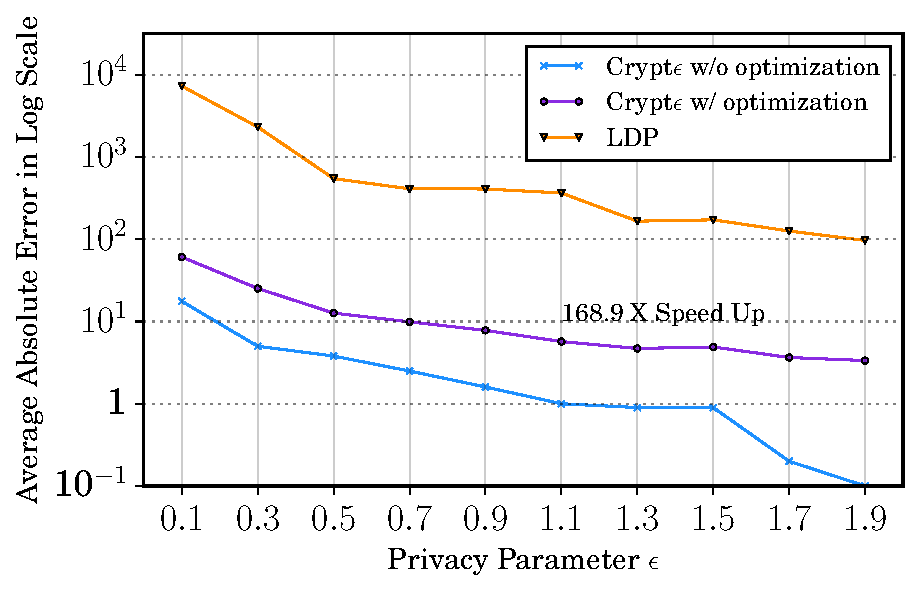
\includegraphics[width=5cm,height=3.1cm]{t1.pdf}
         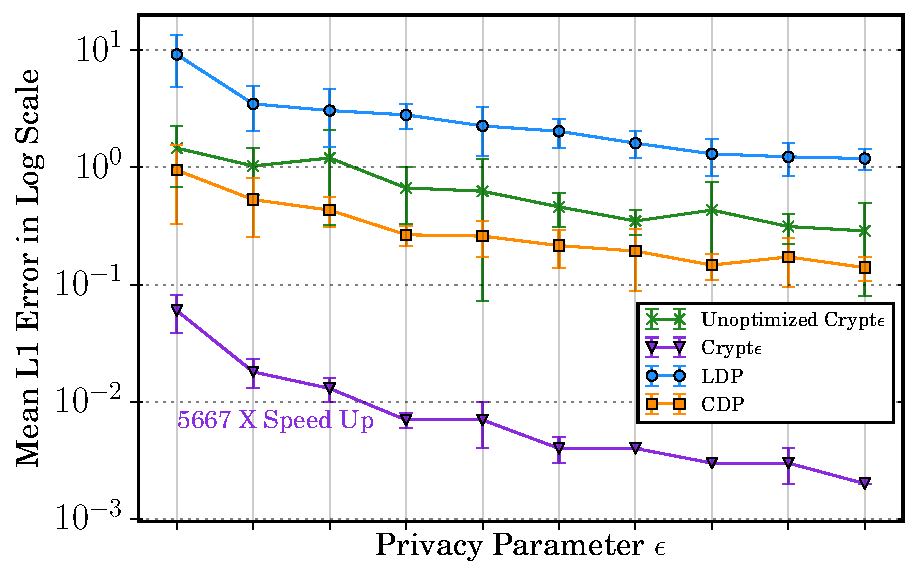
\includegraphics[width=1\linewidth]{8_final.pdf}
        \caption{ Program 1}
        \label{fig:P1}
    \end{subfigure}%%
    \begin{subfigure}[b]{0.25\linewidth}
    \centering 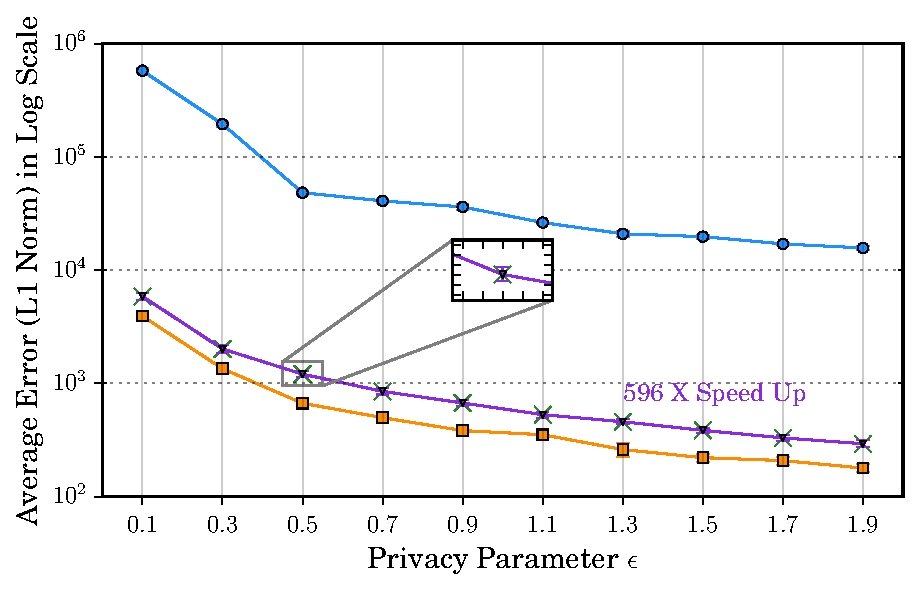
\includegraphics[width=1\linewidth]{3_final.pdf}
        \caption{Program 3}
        \label{fig:P3}\end{subfigure}%%
    \begin{subfigure}[b]{0.25\linewidth}
    \centering    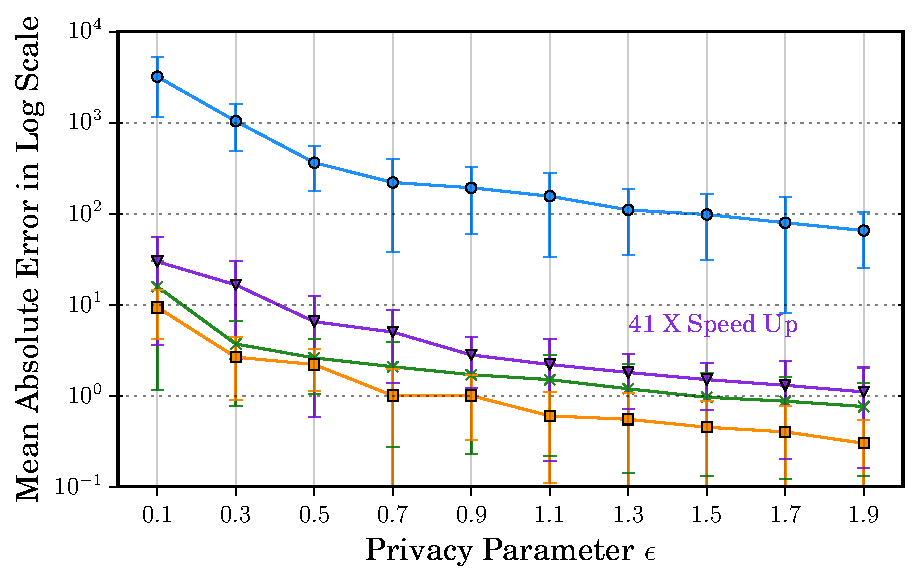
\includegraphics[width=1\linewidth]{5_final.pdf}
        \caption{Program 5}
        \label{fig:P5}\end{subfigure}%%
      \begin{subfigure}[b]{0.25\linewidth}
    \centering    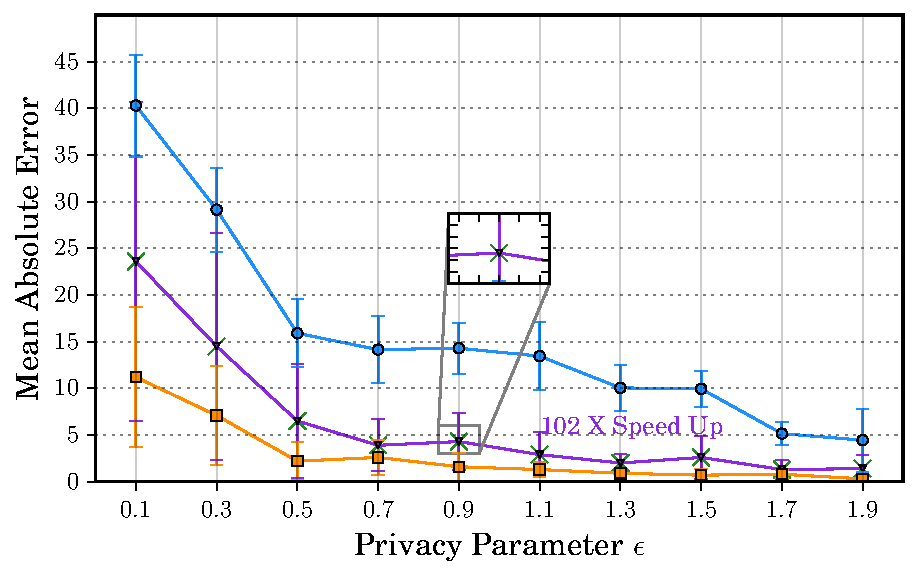
\includegraphics[width=1\linewidth]{7_final.pdf}
        \caption{Program 7}
        \label{fig:P7}
    \end{subfigure}
   \caption{Accuracy Analysis of Crypt$\epsilon$ Programs}
   \label{accuracy}
\end{figure*}
In this section we describe our evaluation of Crypt$\epsilon$ along two dimensions, accuracy and  performance of Crypt$\epsilon$ programs. Specifically, we address the following questions : \squishlist \item \textbf{Q1:} Do Crypt$\epsilon$ programs have significantly lower error than that for the corresponding state-of-the-art \textsf{LDP} implementations? Additionally, is the accuracy of \system programs comparable to that of the corresponding \textsf{CDP} implementations? \item \textbf{Q2:} Do the proposed optimizations provide substantial performance improvement over unoptimized Crypt$\epsilon$? \item \textbf{Q3:} Is the execution time for Crypt$\epsilon$ programs practical and scalable? \squishend
%For the rest of the section, we consider the optimized implementation to be the default implementation for \system.\\
\textbf{Evaluation Highlights:}
\squishlist \item \system can achieve upto 2 orders of smaller error than the corresponding
\textsf{LDP} implementation on a data of significant size ($\sim 30,00$) (Figure \ref{accuracy}).
\item The optimization techniques in \system can improve the running time
of unoptimized \system by up to $6514\times$ (Table \ref{perf}).
\item The performance cost of a large class of \system programs is
less than 5 minutes for a dataset of size $\sim 30,000$  and it scales linearly with the size of the dataset (Figure \ref{scale}). The \textsf{AS} performs majority of the work for most program executions (Table \ref{perf}).
\squishend
\subsection{Methodology} 
\textbf{Programs:}
To answer the aforementioned questions, we ran the experiments on the Crypt$\epsilon$ programs previously outlined in Table 3. Due to space limitations we present the results of only four of them in the main paper namely P1,P3,P5 and P7. The rationale behind choosing these four is that they cover all three classes of programs (section 5.3) and showcase the advantages for all of the four proposed optimizations. %Each program is compared with the corresponding state-of-the-art \textsf{LDP} implementation \cite{LDP1}.
Additional experimental results for programs P2,P4 and P6 from Table \ref{tab:programexamples} are presented in Figure .% We rename the examples 5.1,5.2,5.3,5.4,5.6 and 5.7 as P1,P1,P5,. The reason behind this grouping is to arrange the programs in their increasing order of complexity.  %\begin{itemize}\item \textbf{Program 1} - Count the number of records having age in range $[50,60]$ \\\textbf{\textsf{LDP} Competitor} - Frequency oracle of \cite{LDP1} constructed over attribute $Age$. \item \textbf{Program 2} - Report the top 5 most frequent age values. \\\textbf{\textsf{LDP} Competitor} - Frequency oracle of \cite{LDP1} constructed over attribute $Age$.  \item \textbf{Program 3 }- Report the marginal on attributes $Age$ and $Gender$. \\\textbf{\textsf{LDP} Competitor }- Frequency oracle of \cite{LDP1} constructed over attribute $Age \times Gender$. \item \textbf{Program 4 }- Report the marginal on attributes $Age$ and $Gender$ with $NativeCountry=Mexico$\\\textbf{\textsf{LDP} Competitor }- Frequency oracle of \cite{LDP1} constructed over attribute $Age\times Gender \times NativeCountry$. \item \textbf{Program 5 }- Count the number of natively Mexican male employees of age 30.\\\textbf{\textsf{LDP} Competitor }- Frequency oracle of \cite{LDP1} constructed over attribute $Age\times Gender \times NativeCountry$. \item \textbf{Program 6 }- Count the number of distinct age values for male employees. \\\textbf{\textsf{LDP} Competitor }-Frequency oracle of \cite{LDP1} constructed over attribute $Age\times Gender$.% and reports the number of non-zero counts after suitable adjustment for thresholding. 
%\item \textbf{Program 7 }- Count the number of age values with at least 10 records. \\\textbf{\textsf{LDP} Competitor }- Frequency oracle of \cite{LDP1} constructed over attribute $Age$. \end{itemize}
\\\textbf{dataset:}
We ran our experiments on the Adult dataset from the University of California, Irvine repository \cite{UCI}  which has been extracted from the 1994 census data. The dataset is of size $32,651$.
\\\textbf{Metrics:}
\\\textit{Accuracy:} For accuracy the following metrics are used
\squishlist \item Programs with scalar outputs, i.e.,  P5 and P7 use absolute error $ =|c-\hat{c}|$ where $c$ is the true count and $\hat{c}$ is the noisy output.\item Programs with vector outputs, i.e., P1 and P3 uses the L1 error metric given  by $Error=\sum_{i}|V[i]-\hat{V}[i]|, i \in [|V|]$.\\
For each of the programs, we report the mean error values over 10 repetitions.\squishend
\textit{Performance}: For measuring performance we report the mean total execution time in seconds for each program over 10 runs. \textbf{Configuration:} We implemented \system in Python with the garbled circuit implementation of  the EMP
toolkit \cite{EMP}. The prototype  includes all four 
optimizations described in section 6.
For Adult dataset, \system constructs a DP index optimization over
the attribute $NativeCountry$ that benefits programs like P4 and P5. Our experiments assign
20\% of the total program privacy parameter towards constructing the index
and the rest is used for the remaining program execution. \system also constructs a
DP range tree over the attribute $Age$ with the full privacy parameter. This helps programs like P1,P2 and P3. This is our default implementation for \system. %We refer to the implementation without the optimization as  unoptimized \system. 
% We evaluated our prototype on 3 servers each with configuration 32GB RAM, 1TB SSD, and
%2.6GHz 6-core 8th-generation Intel Core i7 processor and  macOS.

%uses the error measure given by the fraction of age values returned in the top 5 that have value less than $ct_5-\alpha$  where  $ct_5$ is the count of the $5^{th}$ largest value and $\alpha=\frac{1}{\epsilon}\log\frac{1}{\delta}$ is a slack parameter. The slack parameter is required because with probability $1-\delta$ no differentially private algorithm can distinguish between any two counts that differ by less than $\alpha$. We use $\delta=0.05$ for our experiment. \item Programs 3, 4 and 5 \end{itemize}


\subsection{Experimental Results}\label{exp:results}
\subsection*{Accuracy}
In this section we evaluate \textbf{Q1} by performing a comparative analysis between the empirical accuracy of the aforementioned four \system programs (both optimized and unoptimized) and that of the corresponding state-of-the-art \textsf{LDP} \cite{LDP1} and \textsf{CDP} \cite{Dork} implementations  with varying privacy parameter $\epsilon \in \{0.1,...,0.9\}$. %All the experiments are evaluated on the full dataset and we report our results for 
The first observation with respect to accuracy is that the mean error for a single frequency count for Crypt$\epsilon$ is at least 2 orders less than that of the corresponding \textsf{LDP} implementation.   For e.g., Figure \ref{fig:P1} shows that for P1 (c.d.f on $Age$), the mean error for \system for $\epsilon=0.1$ is given by $0.060$ while the corresponding \textsf{LDP} implementation has an error of $9.2$. Similarly for P3 (Figure \ref{fig:P3}),  $\epsilon=0.1$ results in a mean error of $5862.4$ as compared to an error of $576478.2$ for the corresponding \textsf{LDP} implementation. P5 (Figure \ref{fig:P5}) gives a mean error of only $15.8$ for $\epsilon=0.1$. In contrast, the corresponding \textsf{LDP} implementation has an error of $3199.96$.   The accuracy
improvement on P7 (Figure \ref{fig:P7}) by \system is less significant as compared to the other programs. This is so because P7 outputs the number of age values ([1-100]) having at least
100 records. At $\epsilon=0.1$, at least 40 age values out of 100 are
reported incorrectly on whether their counts pass the threshold. \system reduces the error by half. 

For P1 (Figure \ref{fig:P1}), we observe that the error of \system is around an order less than that of the unoptimized implementation. For instance, the mean error for \system is $20\times$ lower than that of unoptimized \system for $\epsilon=0.1$.  The reason is that P1 constructs the c.d.f over the attribute $Age$ (with domain size 100) by first executing 100 range queries. %, where the $i$-th query outputs the noisy count for age values in $[1,i], i \in [100]$. This is followed by an isotonic regression post-processing to get a proper c.d.f.
Thus, if the total privacy budget for the program is $\epsilon$, then for unoptimized \system, each query gets a privacy parameter of just $\frac{\epsilon}{100}$. In contrast, the DP range tree is constructed with the full budget $\epsilon$ and sensitivity $\lceil\log 100\rceil$ thereby resulting in lesser error. For P5 (Figure \ref{fig:P5}) however, the unoptimized implementation has slightly better accuracy (around $2\times$) than \system. It is because of two reasons; firstly the noisy index on $NativeCountry$ might miss some of the rows satisfying the filter condition ($NativeCountry$=Mexico). Secondly, since only 0.8\% of the total privacy parameter is budgeted for the \textsf{Laplace} primitive in the optimized program execution, this results in a higher error as compared to that of unoptimized \system. However, this is a small  cost to pay for achieving a performance gain of $41\times$. The optimizations for P3 (Figure \ref{fig:P3}) and P7 (Figure \ref{fig:P7}) work completely on the encrypted data and do not expend the privacy budget. Hence they do not hurt the program accuracy in any way.
 
 Another observation from Figure \ref{accuracy} is that the error of \system is around $2\times$ higher than that of the corresponding \textsf{CDP} implementation. This conforms with our expectation as we add two instances of Laplace noise in \system. For instance, \system's error for programs 4 (Figure \ref{fig:P3}), 6 (Figure \ref{fig:P5}) and 8 (Figure \ref{fig:P7})  is respectively $1.49\times$, $1.69 \times$ and $2.1\times$ higher  than that of the corresponding \textsf{CDP} implementation for $\epsilon=0.1$.  For P1 however, \system has at least $15\times$ lower error than that of the \textsf{CDP} implementation due to the DP range tree optimization as explained in the preceding paragraph.
 

\subsection*{Performance Gain Due to Optimizations}
In this section we evaluate \textbf{Q2} by analysing how much speed-up is brought about by the proposed optimizations in the total program execution. The results are reported in Table \ref{perf}.
 \eat{\begin{table}[ht]
\caption{Execution Time Analysis for Crypt$\epsilon$ Programs}
\small
\centering
\begin{tabular}{c  c c c c c}
\toprule
Program &  \multicolumn{3}{c}{Base} & \multicolumn{2}{c}{Optimized} \\ 
 & AS &  CSP & Total & Total & Speed up  \\ &(s)&(s)&(s)&(s)&$\times$\\ % inserts table %heading
\midrule
1 & 0.49& 0.0027& 0.4927 & 0.0029 & 168.9 \\
2 &  6.12 & 0.3  &6.42 & 0.89 & 7.2\\ %197 the communication rounds
3&  3859.52 & 3661.29 & 7520.81&N/A&N/A \\4  &7765.16&3624.05&11389.21& 910.96 & 12.5 \\5&18.56&16.7&35.26&3.49 & 10.1 \\6&1910.01&571.11&2481.12&429.92 & 5.77\\7&6.35 & 1393.89 & 1400.24 &  N/A & N/A \\ [1ex]
\bottomrule
\end{tabular}
\label{c}
\end{table}}
\begin{table}
\caption{Execution Time Analysis for Crypt$\epsilon$ Programs}
\centering
\scalebox{0.78}{
\begin{tabular}{|c c|c|c|c|c|}
\hline
\multicolumn{2}{|c}{\textbf{Time in (s)}}   & \multicolumn{4}{|c|}{\textbf{Program}}\\
\cline{3-6}&&\textbf{1} & \bf{3} & \bf{5} &\bf{7}  \\ 
\hline \hline
\multirow{3}{*}{\textbf{Unoptimized \system}}& \multicolumn{1}{|c|}{\textsf{AS}} & 1756.71 &  101840.83 & 650.78&290   \\
\cline{2-6}& \multicolumn{1}{|c|}{\textsf{CSP}} & 0.26 & 78131.27& 550.34  &30407.73\\\cline{2-6}
& \multicolumn{1}{|c|}{Total} & 1756.97 & 179972& 1201.12 &30697.73    \\\hline
%\multirow{4}{*}{\textbf{Optimized}}& \multicolumn{1}{|c|}{\textsf{AS}} & .0004 &16.21 &250.17  &\\ \cline{2-6}& \multicolumn{1}{|c|}{\textsf{CSP}} & .0027 &13.92 &0.54 &\\
\multirow{2}{*}{\textbf{\system}}& \multicolumn{1}{|c|}{Total} & 0.31 &     301.53 & 29.21& 299.5 \\
\cline{2-6}& \multicolumn{1}{|c|}{Speed Up $\times$} &5667.64 &596.86& 41.1 &    102.49
\\ [1ex]
\hline
\end{tabular}}
\label{perf}
\end{table}
\\
\textit{DP Range Tree}
 For P1 we see that the total time taken for execution for the unoptimized Crypt$\epsilon$ implementation is about half an hour. However, using the range tree optimization reduces the execution time by $5667\times$. The reason behind this huge speed-up is that the time required by the \textsf{AS} in the optimized implementation becomes almost negligible because it simply needs to do a memory fetch to read off the answer from the pre-computed range tree instead of computing it from the entire encrypted database. 
 \begin{figure}[ht]
   \begin{subfigure}[b]{0.45\linewidth}
    \centering 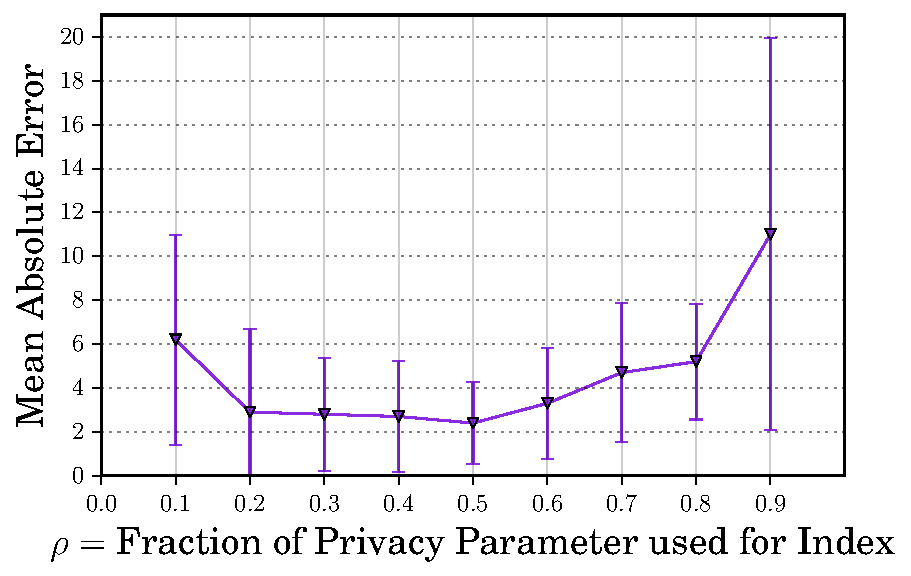
\includegraphics[width=1\linewidth]{index_error.pdf}
        \caption{}
        \label{fig:error}\end{subfigure}
        \begin{subfigure}[b]{0.45\linewidth}
        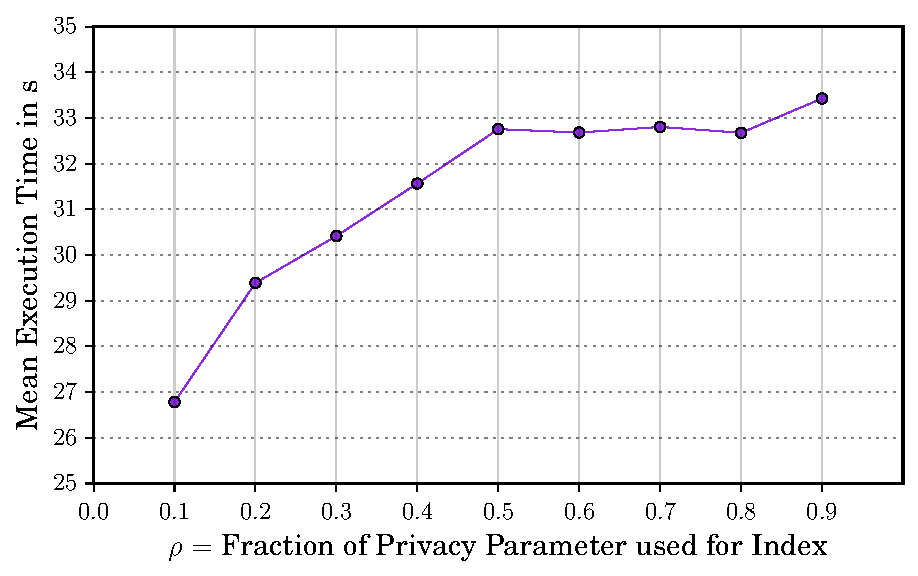
\includegraphics[width=1\linewidth]{index_time.pdf}
        \caption{}
        \label{fig:time}
        \end{subfigure}
        \caption{Program 5: Accuracy vs Performance Trade-off Analysis for DP Index Optimization }\label{index}
    \end{figure}
\\\textit{DP Index}- For P5, we observe that the base case implementation takes around $20$ minutes to run. However,  a DP index over the attribute $NativeCountry$  reduces the execution time to about $30s$ giving us a $41\times $ speed-up. This is because only about 2\% of the data records satisfy $NativeCountry$=Mexico. Thus the index reduces the number of records to be considered for the program execution drastically thereby resulting in a huge performance boost. %The is because only the cost for the \textsf{Filter} primitive decreases, not all the primitives scale 10 drop is due to the 
Let $\rho$ represent the fraction of the privacy parameter used towards constructing the DP index. In Figure \ref{index} we study how the mean execution time and the error of the final result vary as a function of $\rho$ for P5 for a total privacy parameter of $\epsilon=1.1$.  From Figure \ref{fig:error} we observe that the mean error incurred drops sharply from $\rho=0.1$ to $\rho=0.2$, stabilises till $\rho=0.5$ and starts increasing again. This is so because at $\rho=0.2$, the noisy index correctly identifies almost all the records satisfying the $\textsf{Filter}$ condition and hence does not contribute much to the total error. However, as we keep increasing $\rho$, the amount of privacy budget left for the $\textsf{Laplace}$ primitive keeps decreasing which results in higher error. From Figure \ref{fig:time}, we observe that the execution time increases till $\rho=0.5$ and then stabilizes. The reason behind this is that, the total number of records returned after $\rho=0.5$ does not differ by much. Thus from the two figures we observe that for $\rho=0.2$ we get a high speed up ($40\times$) with relatively low error ($3$). Hence we choose $\rho=0.2$ for our experiments. A formal accuracy vs speed up trade-off analysis would be very helpful in this regard and is part of our future plan.
 \\\textit{Pre-computation}- For P3 the unoptimized execution time on the dataset of $32561$ records is around 2 days. This is so because the $\textsf{CrossProduct}$ primitive used in the program needs to perform $200\cdot 32561$ $labMult$ operations which is very time consuming. Hence from Table \ref{perf} we see that, pre-computing the 2-D attribute over $Age$ and $Gender$ is a very useful optimization as now the execution reduces to just about 5 minutes giving us a $596.86\times$ speed up. \\ %The un-optimized implementation for  Program D takes . It is because of the \textsf{CrossProduct} Primitiev because ot needs to compute . Pre-computaion f thsi saves a lot of time and cuts down the executioj tiem by.
\textit{Off-line Processing}-
The costliest primitive for P7 is the \textsf{GroupByCount} primitive since the \textsf{CSP} has to generate $3256200$ ciphertexts of $0$ and $1$ for the encrypted one-hot-codings. This results in a  total execution time of about 8.5 hours in unoptimized \system. However, by generating the ciphertexts off-line, the execution time can be reduced to just $5$ minutes giving us a speed up of $102.49\times$.
Another important observation from Table \ref{perf} is that the \textsf{AS} performs the major chunk of the work for most program executions. This conforms with our discussion in section 3.6.
 \begin{figure}[ht]
    
     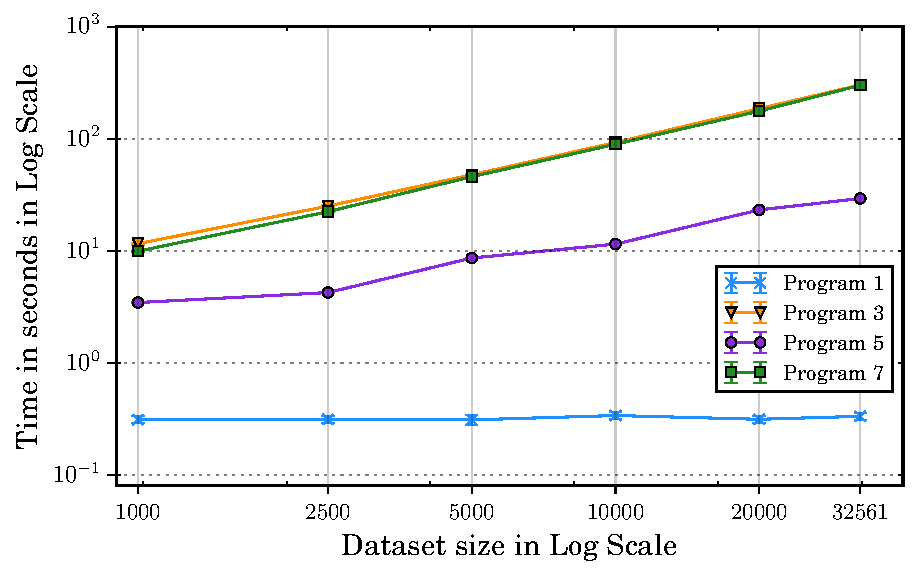
\includegraphics[width=0.5\linewidth]{scale_finals.pdf}
        \caption{Scalability of \system Programs }\label{scale}
    \end{figure}
 \subsection*{Scalability}
 In this section we evaluate \textbf{Q3} by observing the execution times of the aforementioned four \system programs and studying how well the programs scale (Figure \ref{scale}). All the reported execution times are for optimized implementations. For P1 we see that the the execution time remains unchanged with increase in the dataset size. This is so because once the range tree is constructed, irrespective of the dataset size, the program execution just involves reading the answer directly from the nodes of the tree followed by a decryption by the \textsf{CSP}. The execution time for the optimized P3 is dominated by the cost of the $\oplus$ operation for the \textsf{GroupBy} primitive which scales linearly with the number of data records. Hence, as shown in Figure \ref{scale}, the execution time for P3 increases linearly with the dataset size. For P5, the execution time basically depends on the \% of the records in the dataset that satisfy the condition $NativeCountry=Mexico$ (as this is roughly the number of records that will be retrieved from the noisy index). %From the figure, we observe that P5 too scales almost linearly with the dataset size. 
 For the optimized execution of P7  as well, the time is dominated by the $\oplus$ operation for the \textsf{GroupBy} primitive, thereby scaling linearly with the dataset size.   %\subsection{Threats to Validity}- 
 %In Table 2 we report the execution time of  the aforementioned $7$ Crypt$\epsilon$ programs. For Program 1 we see that the total time taken for execution for the base case Crypt$\epsilon$ implementation is about 0.5 seconds; the cost is mainly dominated by the \textsf{AS} which has to make a pass through the entire encrypted database. The \textsf{CSP} on the other hand is just needed for decryption in the last step. Program 2 needs to compute the encrypted $Age$ histogram via $GroupBy*$ primitive which takes about $6$ seconds. The \textsf{CSP} time is also more than the previous case because of the garbled circuit in the $NoisyMax$ primitive. The total execution time for the base case implementation for Program 3 is roughly 2 hours.  The reason behind this comparatively higher timing as compared to that of the previous two programs is that the \textsf{CrossProduct} primitive requires  multiplication of the ciphers  which is costlier than the addition operator $\bigoplus$. For Program 4, we observe that the base case implementation takes around 3.1 hours to run. The timing is greater than that for Program 3 because, in this case the additional condition $NativeCountry=Mexico$ results in extra interactions with the \textsf{CSP}. Program 5 requires about $35$ seconds to execute in the base case while Program 6 runs for $41$ minutes. For Program 7 we see that the majority of the time is required by the \textsf{CSP} for generating the encrypted one-hot-codings for the $GroupBy$ primitive and takes $24$ minutes to execute.  An important observation throughout the experiments is that the time taken by the \textsf{AS} is significantly greater than that for the \textsf{CSP} for all the programs except for Program 7. This is a desirable trait for Crypt$\epsilon$ as discussed in section 3.6.









\section{Related Work}\label{sec:related-short}
\textit{Differential Privacy }- Introduced by Dwork et al. in \cite{Dork}, differential privacy has enjoyed immense attention from both academia and industry in the last decade. Some of the most recent directions in the \textsf{CDP} model include \cite{MVG,Blocki,AHP,DAWA,hist1,hist2,hist3,hist4,hist6,hist7,hist8,A1,A2,A3,A4,A5,A6,A7,A8,u1,u2,MWEM}. The most prominent work in \textsf{LDP} include \cite{LDP1, LDP2, Rappor1,HH,Rappor2,HH2,Cormode, CALM,15,itemset}.
Recently, it has been showed that augmenting the local differential privacy setting by an additional layer of anonymity can improve the privacy
guarantees (or equivalently decrease error bound) \cite{mixnets,Prochlo,amplification}.  An important point to be noted here is that the power of this new model (known as shuffler/mixnet model) lies strictly between that of traditional \textsf{LDP} and \textsf{CDP}. The two-server model of Crypt$\epsilon$ differs from this line of work in three ways. Firstly, Crypt$\epsilon$ results in no reduction in expressibility as compared to that of the \textsf{CDP} model (see Appendix \ref{app:sepldp}). Secondly, the shuffler/mixnet model results in an approximate DP guarantee $(\epsilon\sqrt{\frac{\log\frac{1}{\delta}}{n}},\delta)$ which incurs an expected error of $O(\epsilon\sqrt{\log\frac{1}{\delta}})$.  In practice, $\delta$ has to be at least $\frac{1}{n}$ in order to get meaningful privacy. In contrast Crypt$\epsilon$ achieves the the same order of accuracy guarantees as that of \textsf{CDP}. Finally, the shuffler/mixnet model and \system have certain differences in their respective trust assumptions. For more details see Appendix D.2. %Google's implementation relies on a trusted intermediary shuffler which they implement via trusted hardware enclaves. However truly secure hardware enclaves are notoriously difficult to achieve in practice \cite{Foreshadow}. The mixnet model on the other hand requires a  mix network or mixnet which is a protocol involving several computers that inputs a sequenceof encrypted messages, and outputs a uniformly random permutation of those messages' plaintexts.  Their trust assumption is that at least one of the servers needs to behave honestly. For Crypt$\epsilon$ both the servers are completely untrusted under the constraint that they are non-colluding and follow the protocols semi-honestly.
\\\textit{Two-Server Model} - The two-server model is a popular choice especially for privacy preserving machine learning approaches where typically one of the servers manages the cryptographic primitives while the other handles computation. Examples of this include \cite{Boneh1,Boneh2,Ridge2,Matrix2,secureML,LReg,Ver}. \\\textit{Homomorphic Encryption } - Recently, there has been a surge in  privacy preserving solutions using homomorphic encryptions due to improved primitives. A lot of the aforementioned two-server models employ homomorphic encryption \cite{Boneh1,Boneh2,LReg,Matrix2}.  Additionally it is used in \cite{CryptoDL,CryptoNet,NN, Irene2, grid}.
%A detailed discussion on related work is presented in  Appendix \ref{app:related}.



\section{Conclusions}\label{sec:conclusions}
%There are a number of future work directions for Crypt$\epsilon$. 
In this paper we have proposed a new implementation model for differential privacy that achieves the constant error bound and  algorithmic expressibility of \textsf{CDP} without the need for any trusted party. This is achieved via two non-colluding servers with the assistance of cryptographic primitives specifically \textsf{LHE} and garbled circuits. Our proposed system \system can execute a rich class of programs that can run  efficiently by virtue of four optimizations.
\par  One possible extension of the current work can be the development of a
Crypt$\epsilon$ compiler. Recall that currently the data analyst spells out the explicit Crypt$\epsilon$ program  (i.e., the sequence of Crypt$\epsilon$ primitives and their arguments) to the \textsf{AS}. Thus a useful future work can be constructing a compiler that takes as input only a user specified query in a high-level-language and a total privacy budget for the query. The
compiler should then be able to formalize an optimized Crypt$\epsilon$ program expressed in terms of Crypt$\epsilon$ primitives with automated sensitivity analysis and subsequent optimal per measurement primitive privacy budget allocation. 
Another very logical future work can be to support a larger class of programs in \system. For e.g., extension of the current functionality of \system to include aggregation operators such as sum, median, average etc should be easily achievable. Supporting  multi-table queries like joins in \system based on existing works along the lines of \emph{elastic sensitivity} \cite{elastic} etc would also be an useful extension.  Yet another interesting direction can be enabling learning algorithms on \system.   Comparatively simpler algorithms like linear regression can based on a previous work \cite{LReg} which also uses \textsf{LHE} and a two-server model. For this, we need to extend \system with a new primitive that performs matrix multiplications. For more involved models like deep learning, we might need to combine the differential privacy results of \cite{DLDP} with the homomorphic encryption techniques of  CryptoNet \cite{CryptoNet}. As mentioned in section 3.6, an alternative implementation for \system  can be based on secret shares modulo the assumption that both the servers are benefit from learning the differential privacy output. Hence another useful extension might be re-implementing \system with  secret shares. For this, the functionality of the existing primitives would mostly be the same, only the respective implementations will change. 
Yet another extension can be removing the second server (\textsf{CSP}) altogether and instead capturing its functionalities within a trusted execution environment (TEE) as mentioned in Section 7.2.

%\bibliographystyle{ACM-Reference-Format}
\bibliographystyle{abbrv}
\bibliography{references.bib}
\appendix

\subsection{Security Proof}
\begin{proof}
Recall any program in \system is a sequence of transformation primitives followed by either a $\textsf{Laplace}$ primitive or a \textsf{NoisyMax} primitive. First we prove for the case when program $P$ uses Laplace mechanism.

As discussed in section 4.2 and 4.3, the sensitivity of a \system program is computed as the product of the stabilities of the transformation primitives used in it.
Let the equivalent \system program for $P$ be denoted as $P_{\system}$
\textbf{Correctness:}
 Using the homomorphic properties of the underlying encryption
scheme, it easy to verify that at the end of performing all the transformation primtives the \textsf{AS} knows $P(D)+$.  Now clearly 
Let simulators $Sim_1$ and $Sim_2$ simulate the view of ${Adv}_1$ and $Adv_2$ respectively. 
Let $l$ be the bit-length of each data record represented in per-attribute one-hot-coding. \\
First we prove for the case when $P$ uses Laplace mechanism.
$\mathcal{S}_1=Sim_1(\{D_i, i \in S\}, P,\Delta=1,\epsilon, P(\mathcal{D})+\eta_2,P(\mathcal{D})+\eta_1)$
\begin{enumerate}\item Run $Gen(\kappa)\mapsto (pk,sk)$ 
\item Draw $\eta' \in Lap(\frac{1}{\epsilon})$
\item For all $i \in \{1,...,m\}$ if $i \in S$ then encrypt $D_i$. 
Otherwise compute $labEnc_{pk}(D_i)$ as a random $l$-lengthed vector $r_i \in \mathcal{C}^l$. [We abuse the notation slightly here, $labEnc_pk(D_i)$ denotes component wise encryption of the record represented in per-attribute one-hot-coding]
\item Output $\Big(\{D_i, i \in S\},P,\Delta=1,\epsilon,\eta',\encD',P(\mathcal{D})+\eta_2+\eta'\Big)$ where $\encD'=\{labEnc_{pk}(D_i)\},i \in \{1,...,m\} i \not \in S$ as computed in step 3.
\end{enumerate}
The R.H.S of eq \ref{adv1}  is given by 
\begin{gather}\Big(\{D_i, i \in S\},P,\Delta=1,\epsilon, \eta_1,\encD,P(\mathcal{D})+\eta_2+\eta_1\Big)\end{gather}
It follows from the semantic security of the encryption scheme that $\encD'$ and $\encD'$ are computationally indistinguishable.
Since, $\eta'$ is drawn from the same distribution as $\eta_1$, $P(\mathcal{D})+\eta'+\eta_2$ and $P(\mathcal{D})+\eta_1+\eta_2$ have the exact same distribution. This proves that the distribution of simulation output is computationally indistinguishable from that of the views of the corrupted parties in $Adv_2$
output has the same distribution as that of the views of the corrupted parties in $Adv_1$ in the
protocol $\Pi$.\\
$\mathcal{S}_2=Sim_2(\{D_i, i \in S\},P,\Delta=1,\epsilon,P(\mathcal{D})+\eta_1,P(\mathcal{D})+\eta_2)$
\begin{enumerate}\item Run $Gen(\kappa)\mapsto (pk,sk)$ \item Generate $\eta'' \in Lap(\frac{1}{\epsilon})$ \item Output $\Big\{D_i, i \in S\},P,\Delta=1,\epsilon, \eta'', labEnc_{pk}(P(\mathcal{D})+\eta_1), P(\mathcal{D})+\eta_1+\eta''\Big)$
\end{enumerate}
The R.H.S of eq \ref{adv2} is given by \begin{gather}\Big(\{D_i, i \in S\},P,\Delta=1,\epsilon,\eta_2,labEnc_{pk}(P(\mathcal{D})+\eta_1),P(\mathcal{D})+\eta_1+\eta_2\Big)\end{gather}
Again, clearly the simulation output has the same distribution of the
views of the corrupted parties in $Adv_2$ in the protocol $\Pi$. 
The proof for the case of NoisyMax is inherent from the semantic security of the garbled circuit used (section B.1).
\end{proof}



\section{Additional Implementation Details}\label{app:implement}

\subsection{Primitive Implementation}\label{app:implement_primitives}

\stitle{\textsf{CrossProduct}} $\crossproduct_{A_i,A_j\rightarrow A'}(\cdot)$: This primitive replaces the two attributes $A_i$ and $A_j$ by a single attribute $A'$. Given the encrypted input table $\encT$, where all attributes are in one-hot-encoding and encrypted, the attributes of $\encT$ except $A_i$ and $A_j$ remain the same. For every row in $\encT$, we denote the encrypted one-hot-encoding for $A_i$ and $A_j$ by $\tilde{\bf{v}}_1$ and $\tilde{\bf{v}}_2$.  Let $s_1$ and $s_2$ be the domain sizes of $A_i$ and $A_j$ respectively. Then the new one-hot-encoding for $A'$, denoted by $\tilde{\bf{v}}$, has a length of $s=s_1\cdot s_2$. For $l\in \{0,1,\ldots, s-1\}$, we have $$\tilde{\bf{v}}[l] = labMult(\tilde{\bf{v}}_1[l/s_2], \tilde{\bf{v}}_2[l\%s_2]).$$
Only one bit in $\tilde{\bf{v}}$ for $A'$ will be encrypted 1 and the others will be encrypted 0s. When merging more than two attributes, \system can use the $genLabMult()$ described in Section~\ref{genlab} to speed up computation.


%Let $D_1$ and $D_2$  be the encrypted one-hot-coding corresponding to two  values $v_1$ and $v_2$ (integral representation) for attributes $A_1$ and $A_2$ respectively. The corresponding encrypted one-hot-encoding for the two-dimensional attribute $A_1\times A_2$ is given by  \begin{gather} D_{1\times 2}[(i-1)\cdot s_{A_2}+j] = labMult(D_1[i], D_2[j])\\ i \in [s_{A_1}], j \in [s_{A_2}]\end{gather} For this particular case, only $D_{1 \times 2}[(v_1-1)\cdot s_{A_2}+v_2]=Enc(1)$ while all other indices will equate to $Enc(0)$. Note that when computing the one-hot-encoding for a t-dimensional attribute $t > 2$,  for the actual implementation, instead of calling $t$ iterative instances of \textsf{CrossProduct}() we use the $genLabMult()$ operator of labeled homomorphic encryption to speed up the computation.

\stitle{\textsf{Project}} $\project_{\bar{A}}(\cdot)$: The implementation of this primitive simply drops off all but the attributes in $\bar{A}$ from the input table $\encT$ and returns the truncated table $\encT'$.

\stitle{\textsf{Filter}} $\filter_{\phi}(\cdot)$: The predicate $\phi$ in this primitive is a conjunction of range conditions over $\bar{A}$, defined as: for a row $r$ in input table $\encT$,
$\phi(r) = \bigwedge_{A_j\in \bar{A}} ~~(r.{A_j} \in V_{A_j}),$ where $r.A_j$ is the value of attribute $A_j$ in row $r$ and $V_{A_j} \subseteq \{0,1,\ldots,s_{A_j}\}$ (the indices for attribute values of $A_{j}$ with domain size $s_{A_j}$).

First, we will show how to evaluate whether a row $r$ satisfies $r.{A_j} \in V_{A_j}$. Let $\tilde{\bf{v}}_j$ be the encrypted one-hot-encoding of $A_j$, then the indicator function can be computed as
$$I_{r.{A_j}\in V_{A_j}}=\bigoplus_{l\in V_{A_j}}\tilde{\bf{v}}_j[l].$$
If the attribute of $A_j$ in $r$ has a value in $V_{A_j}$, then $I_{r.{A_j}\in V_{A_j}}$ equals $1$; otherwise, $0$.

Next, we can multiply all the indicators using $genLabMult()$ (Section~\ref{genlab}) to check whether all attributes in $A_j\in \bar{A}$ of $r$ satisfy the conditions in $\phi$. Let $\bar{A} = \{A_1,\ldots,A_m\}$, then $$\phi(r) = genLabMult(I_{A_1\in V_{A_1}},\ldots, I_{A_m\in V_{A_m}}).$$

Last, we update the bit of $r$ in $\encB$, i.e., $\encB'[i] = labMult(\encB[i], \phi(r))$, given $r$ is the $i$th row in the input table. This step zeros out some additional records which were found to be extraneous by some preceding filter conditions.

Note that when the \textsf{Filter} transformation is applied for the very first time in a \system program and the input predicate is conditioned on a single attribute $A \in V_A$, we can directly compute the new bit vector using $I_{r.A\in V_{A}}$, i.e., for the $i$th record $r$ in input table $\encT$, we have $\encB'[i] =\bigoplus_{l\in V_A} \tilde{\bf{v}}_j[l]$.  This avoids the unnecessary multiplication $labMult(\encB[i],\phi(r))$.


%As discussed in the preceding section, the predicate $\phi$ is expressed in a special form of conjunctions of range conditions given by eq \ref{phi}. Now for a range condition $A \in \{v_1,...v_t\}$, assuming $\mathbf{\tilde{R}_A}[i]$ is the corresponding one-hot-coding for the $i^{th}$ record's value for attribute $A$,  consider the following \begin{gather}\mathbf{c}_A^i=\bigoplus_{j=1}^{t}\tilde{\mathbf{R}}_{A}[i][v_1]\end{gather} where $\tilde{\mathbf{R}}_{A}[i][v]$ is the $v^{th}$ index of corresponding one-hot-coding. Clearly if the $i^{th}$ record satisfies the condition $A \in \{v_1,...v_t\}$, then exactly one of the values in $\{\tilde{\mathbf{R}}_{A}[i][v_j]\}, j \in \{1,...,t\}$ will be a cipher for $1$. Thus $c_A^i=1$ if record $i$ satisfies the range condition and 0 otherwise. If the condition is instead an equality predicate $A==v$ then $\mathbf{c}_A^i=\tilde{\mathbf{R}}_{A}[i][v]$. Now considering $\phi$ is given by eq \ref{phi}, let us define\begin{gather}\mathbf{c}^i=genLabMult(\mathbf{c}^i_{A_1},...,\mathbf{c}^i_{A_r})\\A^*=\bigcup_{j=1}^rA_j\end{gather} It is easy to see that $c^i$=1 iff record $i$ satisfies $\phi$. Let $\mathbf{B}'$ be the indicator vector before the execution of the current instance of the \textsf{Filter} transformation. The final step is to multiply the $\mathbf{c}^i$s with the corresponding indicator bits and obtain the updated indicator vector $\mathbf{B}$ as follows \begin{gather}\mathbf{B}[i]=labMult(\mathbf{c}^i,\mathbf{B}'[i])\end{gather}
%The above step zeros out some additional records which were found to be extraneous by some preceding filter conditions. Clearly $\textbf{B}$ is the output of the \textsf{Filter} transformation.


%Avoid Indicator Vector Multiplication

%When the \textsf{Filter} transformation is applied for the very first time in a Crypt$\epsilon$ program and the input predicate is conditioned on a single attribute $A \in \{v_1,...,v_k\}$, then we can do the following optimization. Consider \begin{gather}\mathbf{b}[i]=\bigoplus_{j=1}^k \mathbf{\tilde{R}}_A[i][v_j], i \in [m]\end{gather} where $\mathbf{\tilde{R}}_A[i]$ is the one-hot-coding for attribute $A$ for the $i^{th}$ record. Since this is the first instance of the \textsf{Filter} primitive, the current indicator vector $\mathbf{B}$  will be all 1-vector. Thus $\mathbf{b}$ is itself the updated indicator vector  and we can avoid the unnecessary multiplication $labMult(\mathbf{b[i]},\mathbf{B}[i])$.

\stitle{\textsf{Count}} $\countagg(\cdot)$: To evaluate this primitive on its input table $\encT$, \system simply  adds up the bits in the corresponding $\encB$, i.e., $\bigoplus_{i}^m \encB[i]$.

%The \textsf{Count} primitive takes the associated bit vector $\mathbf{B}$ of its input table $\encT$  and simply adds up its entries to return  \begin{gather}\mathbf{c}=\bigoplus_{i=1}^m\mathbf{B}[i]\end{gather}%\item GroupBy*($\mathbf{V},sk$)- This primitive is an extension of the previous GroupBy transformation.

\stitle{\textsf{GroupBy*}} $\groupbystar_{A}(\cdot)$: The implementation steps for \textsf{Project}, \textsf{Filter} and \textsf{Count} are reused here. First, \system projects the input table $\encT$ on attribute $A$, i.e. $\encT_1 = \project_A(\encT)$. Then, \system loops each possible value of $A$. For each value $v$, \system initializes a temporary $\encB_v=\encB$ and filters $\encT'$ on $A=v$ to get an updated $\encB'_v$. Last, \system counts the number of 1s in $\encB'_v$ and release the counts.

\eat{
\begin{enumerate}[label=\alph*)] \item $\mathbf{\tilde{T}}_1$=\textsf{Project}($\mathbf{\tilde{T}}$, $A$) \item $\mathbf{B}$ =  current indicator bit vector \item  for $i = 1:s_A $ \\Intialize bit vector to $\mathbf{B}$  \\$\phi_i= (A==v_{i,A}) $ \\$\hat{\mathbf{T_2}}$ = \textsf{Filter}($\mathbf{\tilde{T}}_1, \phi_i$)\\ $\mathbf{C}[i]$ = \textsf{Count}($\hat{\mathbf{T_2}}$) \\ end for \item Output $\mathbf{C}$ 
\end{enumerate}
}

\stitle{\textsf{GroupByCount}} $\groupbystar_A(\cdot)$: The implementation detail of this primitive is given in the main text (section 5.2).

\stitle{\textsf{CountDistinct}}  $\countdistinct(\cdot)$: The implementation of this primitive involves both \AS and \CPS. Given the input encrypted vector of counts $\encV$ of length $s$, the AS first masks $\encV$ to form a new encrypted vector ${\bf \mathcal{V}}$ with a vector of random numbers $M$, i.e., for $i\in \{0,1,\ldots, s-1\}$,
${\bf \mathcal{V}}[i] = {\encV}[i] \oplus labEnc_{pk}(M[i]).$
This masked encrypted vector is then sent to \CPS and decrypted by \CPS to a plaintext vector $\mathcal{V}$ using the secret key.

Next, \CPS generates a garbled circuit which takes (i) the mask $M$ from the \AS, and (ii) the plaintext  masked vector $\mathcal{V}$ and a random number $r$  from the \CPS as the input. This circuit first removes the mask $M$ from $\mathcal{V}$ to get $V$ and then counts the number of non-zero entries in $V$, denoted by $c$. A masked count $c'=c+r$ is outputted by this circuit. \CPS send both the circuit and the encrypted random number $labEnc_{pk}(r)$  to \AS.

Last, the \AS evaluates this circuit to the masked count $c'$ and obtains the final output to this primitive: ${\bf c} = labEnc_{pk}(c') - labEnc_{pk}(r)$.

\eat{
   ($\mathbf{V},\epsilon$) - The \textsf{CountDistinct} primitive is implemented as follows \begin{enumerate}[label=\alph*)]\item Firstly the \textsf{AS} creates a mask vector drawn uniformly at random from $[m]^{s_A}$, i.e.,  \begin{gather*} M[i] \in_R [m], i \in [|V|]\end{gather*} \item \textsf{AS} masks the encrypted true count vector $\mathbf{V}$  as follows \begin{gather*}\boldsymbol{\mathcal{V}}[i]= \mathbf{V}[i] \oplus labEnc_{pk}(M[i])\end{gather*} and sends it to the \textsf{CSP} \item \textsf{CSP} decrypts the masked encrypted vector as \begin{gather*}\mathcal{V}[i]=labDec_{sk}(\mathbf{V}[i]), i \in [|V|]\end{gather*} \item Next the \textsf{CSP} generates the following garbled circuit that\begin{enumerate}[label=\roman*)]  \item takes the mask $M$ as an input from the \textsf{AS} \item takes a random number $r$  as an input from the \textsf{CSP}\item takes the decrypted masked vector $\mathcal{V}$ as an input from the \textsf{CSP} \item removes the mask $M$ from $\mathcal{V}$ as \begin{gather*}V[i]=\mathcal{V}[i]-M[i], i \in [|V|]\end{gather*}\item  counts the number of non-zero entries of $V$ as C \item adds the laplace noises \begin{gather*}\mathcal{C}=C+r\end{gather*} and returns $\mathcal{C}$ \end{enumerate} \item The \textsf{AS} evaluates the above circuit and gets output $\mathcal{C}$ \item The \textsf{AS} gets $labEnc_{pk}(r)$ from the \textsf{CSP} and generates $labEnc_{pk}(\mathcal{C})$ to compute\begin{gather*}\mathbf{C}=labEnc_{pk}(\mathcal{C})-labEnc_{pk}(r)\end{gather*} \end{enumerate}
}


\stitle{\textsf{Laplace}} $\lap_{\epsilon,\Delta}(\mathbf{V})$: Given an encrypted vector counts $\encV$ of size $s$, both \AS and \CPS have to add Laplace noise in this primitive. Hence, this implementation involves two steps.

First, the \AS adds encrypted Laplace noise vector to $\encV$, i.e., for $i\in \{0,1,\ldots,s\}$, $\hat{\encV}[i]  = \encV[i] \oplus labEnc_{pk}(\eta_i),$ where $\eta_i\sim Lap(\Delta/\epsilon)$. This encrypted noisy vector $\hat{\encV}$ is then sent to the \CPS.

Next, the \CPS decrypts $\hat{\encV}$ using the secret key and add another Laplace noise vector, i.e., for  $i\in \{0,1,\ldots,s\}$, $\hat{V}[i] = labDec_{sk}(\hat{\encV}[i]) +\eta'_i$, where $\eta'~\sim Lap(\Delta/\epsilon)$. This plaintext noisy vector is returned as the final output of this primitive.



\eat{
($\mathbf{V},\epsilon$)- Recall that both \textsf{AS} and \textsf{CSP} have to add Laplace noise to the output in Crypt$\epsilon$. Hence the \textsf{Laplace} primitive has two components. The first component is executed by the \textsf{AS} wherein,
\begin{enumerate} \item \textsf{AS} generates a noisy vector $\eta$ such that $\eta \in [Lap(\frac{1}{\epsilon})]^{|V|}$ \item encrypts $\eta$ and adds it to the input vector as \begin{gather*}\boldsymbol{\eta}=labEnc_{pk}(\eta)\\\mathbf{\hat{V}}[i]=\mathbf{V}[i]\oplus \boldsymbol{\eta}[i], i \in [|V|]\end{gather*} \end{enumerate} This encrypted noisy vector $\mathbf{\hat{V}}$ is the input for the second phase of the \textsf{Laplace} primitive which is executed by the \textsf{CSP} as follows \begin{enumerate}\item Decrypts $\mathbf{\hat{V}}$ \begin{gather*}\hat{V}=labDec_{sk}(\mathbf{\hat{V}})\end{gather*}  \item Generates a noisy vector $\eta'$ such that $\eta' \in [Lap(\frac{1}{\epsilon})]^{|\hat{V}|}$ \item Finally adds the noise $\eta'$ to $\hat{V}$ \begin{gather*}\hat{\mathcal{V}}[i]=\hat{V}[i]+\eta'[i], i \in [|\hat{V}|]\end{gather*} \item Returns $\hat{\mathcal{V}}$ to \textsf{AS} \end{enumerate} 
% Note that in the Crypt$\epsilon$ implementation we need to add two instances of the Laplace noise as opposed to a single instance in the standard central differential privacy setting. After the addition of the first instance of the laplace noise, $\eta$ (by the AS),  the encrypted answer is sent to the CSP. becuse of CSP has only a differential private view Hence the addition of the second instance of the laplace noise can be looked upon as a post-processing step  However and differential privacy is immune to post processing 
}


\stitle{\textsf{NoisyMax}} $\noisymax_{\epsilon,\Delta}^k(\cdot)$: The input to this primitive is an encrypted vector of counts $\encV$ of size $s$. Similar to \textsf{Laplace} primitive, both \AS and \CPS are involved. First,  the \AS adds to $\encV$
an encrypted Laplace noise vector and a mask $M$, i.e., for $i\in \{0,1,\ldots,s\}$,
$\hat{\encV}[i]  = \encV[i] \oplus labEnc_{pk}(\eta_i) \oplus M[i],$
where $\eta_i\sim Lap(\Delta/\epsilon)$. This encrypted noisy, masked vector $\hat{\encV}$ is then sent to the \CPS.

Next, the \CPS decrypts $\hat{\encV}$ using the secret key, i.e., for  $i\in \{0,1,\ldots,s\}$, $\hat{V}[i] = labDec_{sk}(\hat{\encV}[i])$. The \CPS generates a garbled circuit which takes  (i) the noisy, masked vector $\hat{V}$ from the \CPS, and (ii) the mask $M$ from the \AS as the input. This circuit will remove the mask from $\hat{V}$ to get the noisy counts $\hat{V}'$ and find the indices of the top-$k$ values in $\hat{V}'$.

Finally, the \AS evaluates the circuit above and returns the indices as the output of this primitive.


\eat{
($\mathbf{V},\epsilon,k$)- The input to the NoisyMax primitive is an encrypted vector $\mathbf{V}$ where each entry $V[i]$ is a count. The primitive is implemented via the following steps.  \begin{enumerate}
\item First the \textsf{AS} adds noise to the input encrypted vector as follows \begin{gather*} \eta \in [Lap(\frac{1}{\epsilon})]^{|V|}\\\boldsymbol{\eta}=labEnc_{pk}(\eta)\\\mathbf{\hat{{V}}}[i]=\mathbf{V}[i]+ \boldsymbol{\eta}[i], i \in [|V|] \end{gather*} \item Next the \textsf{AS} creates a mask vector $M$ drawn uniformly at random from $[m]^{s_A}$, i.e.,  \begin{gather*} M[i] \in_R [m], i \in [|V|]\end{gather*} \item \textsf{AS} masks the encrypted noisy vector $\mathbf{\hat{V}}$  as follows \begin{gather*}\boldsymbol{\mathcal{V}}[i]= \mathbf{\hat{V}}[i] \oplus labEnc_{pk}(M[i]), i \in [|V|]\end{gather*} and sends it to the \textsf{CSP} \item \textsf{CSP} decrypts the masked encrypted noisy vector as \begin{gather*}\mathcal{V}[i]=labDec_{sk}(\mathbf{\hat{V}}[i]), i \in [|V|]\end{gather*} \item Next, the following garbled circuit is evaluated which
    \begin{enumerate}[label=\roman*]\item takes noisy masked  vector $\mathcal{V}$ as an input from the \textsf{CSP} \item takes mask $M$ as the input from \textsf{AS}  \item removes the mask from  $\mathcal{V}$  as \begin{gather*} \hat{V}[i]=\mathcal{V}[i]-M[i], i \in [|V|]\end{gather*}  \item computes the top $k$ element over  $\hat{V}$ and returns $arg_{\textit{top k}}\max{\hat{V}[i])}$
    \end{enumerate}
    \end{enumerate}
}


\subsection{DP Index Optimization Implementation}\label{app:index-imp}

The DP index optimization can be implemented via a garbled circuit which aims to compute two pieces of information: a sorted encrypted database based on $A$ and a $\epsilon$-differentially private index on $A$. This circuit takes (i) the secret key $sk$ from the \CPS, and (ii) the entire database $\encD$ and the attribute $A$ from the \AS. The attribute $A$ has a domain of size $s_A$ and is uniformly partitioned into $k$ ranges $\{R_1,\ldots, R_i, \ldots, R_{s_A/k}\}$, where $R_i = [\frac{s_A}{k}i, \frac{s_A}{k}(i+1))$.

This circuit first decrypts $\encD$ using the secret key and sorts the decrypted database on attribute $A$ in ascending order. The sorted database is then encrypted again. Then the circuit computes a histogram $V$ on the $k$ ranges of $A$, denoted by $[c_1,\ldots,c_k]$  and perturbs each count with Laplace noise, i.e., $\hat{c}_i = c_i + \eta_i$, where $\eta_i\sim Lap(1/\epsilon)$. The noisy counts $\encV$ are then used to construct a cumulative histogram over $A$, where $\hat{cdf}[i] = \sum_{j=0}^i \hat{c}_i$ and post-processed such that they are in non-decreasing order and non-negative, and $\hat{cdf}[k] = |\encD|$~\cite{cdf}.

Given the differentially private cdf and the sorted database, when a program would like to select rows with $A\in [v_i, v_j]$, we find the ranges that contain $v_i$ and $v_j$ respectively, denoted by $R_i$ and $R_j$. Then we return all records in the sorted database which cover all ranges from $R_i$ and $R_j$. This corresponds to row $(\hat{cdf}[i-1]+1)$ to row $(\hat{cdf}[j])$.




%\xh{@chenghong, double check if the writeup reflects what you implemented.}


\eat{
\begin{enumerate}\item takes the entire database $\boldsymbol{\mathcal{\tilde{D}}}$ as an input and the attribute $A$ as an input from the \textsf{AS}.
\item takes the secret key $sk$ as an input from  the \textsf{CSP} \item Decrypts $\boldsymbol{\mathcal{\tilde{D}}}$ \item Sorts the decrypted database on $A$, i.e., the first $ct_{A,v_1}$ rows are the ones with value $v_1$ for attribute $A$, the next $ct_{A,v_2}$ are  the records with value $v_2$ for attribute $A$ and so on. \item  re-encrypts the sorted database \item Divide the domain of $A$ into $k$ bins such that each bin contains $s_A/k$ consecutive domain values. \item Construct a $k$ lengthed vector $\hat{V}$ such that $\hat{V}[i]=\sum_jct_{A,j}+\eta_i, i \in [k], j \in [\frac{s_A}{k}(i-1)+1,\frac{s_A}{k}i]$ where $\eta_i$ is a random laplace noise drawn from the distribution $Lap(\frac{k}{\epsilon})$ \item Return $\hat{V}$ and sorted $\boldsymbol{\mathcal{\tilde{D}}}_{sort}$\end{enumerate}
}

\subsection{Illustration genLabMult}\label{app:genlabhe}
Figure~\ref{genlab-fig} illustrates how a $n$-way multiplication described in Section~\ref{genlab} can be parallelized. This approach requires a total of $\lceil \log n\rceil$ rounds of communication between \AS and \CPS.

\begin{figure}
\includegraphics[width=\columnwidth]{genLab.png} \caption{ $genLabMult()$ - Batching of multiplicands for \textsf{labHE}} \label{genlab-fig}\end{figure}

\section{Related Work}\label{app:related}
\subsection{Differential Privacy}\label{app:dp}
Introduced by Dwork et al.~\cite{Dork}, differential privacy has enjoyed immense attention from both academia and industry in the last decade. We will  discuss the recent directions in two models of differential privacy: the \textit{centralized differential privacy} (CDP), and \textit{local differential privacy} (LDP).

The \textsf{CDP} model assumes the presence of a trusted server which can aggregate all users' data  before perturb the query answers. This allows the design of a complex algorithm that releases more accurate query answers than the basic DP mechanisms. For example, an important line of work in the \textsf{CDP} model has been towards proposing "derived" mechanisms'' \cite{MVG} or  "revised algorithms" \cite{Blocki} from basic DP mechanisms (like exponential mechanism, Laplace mechanism, etc.). The design of these mechanisms leverages on specific properties of the query and the data, resulting in a better utility than the basic mechanisms.  One such technique is based on data partition and aggregation \cite{AHP,hist1,hist2,hist3,hist4,hist6,hist7,hist8} and is helpful in answering histogram queries. The privacy guarantees of these mechanisms can be ensured via the composition theorems and the post-processing property of differential privacy \cite{Dork}. We would like to build \system that can support many of these algorithms. %Another technique involves non-uniform data weighting where each data sample is weighed based on their query contribution. Research in this line of work include \cite{u1,u2,MWEM}. Yet another popular method is to utilize past/auxiliary information to improve the utility of the query answers. Examples are \cite{A1,A2,A3,A4,A6,A7,A8}.

%Another interesting line of work has been towards developing programming frameworks to enable non-experts to write easy differentially private programs. This line of work was started by the PINQ platform \cite{PINQ} and there has been a series of follow up work  \cite{FWPINQ,p2, airavat}. The most recent one is the Ektelo \cite{ektelo} framework where all existing algorithms for answering linear counting queries can be expressed as a composition of its operators. 

The \textsf{LDP} was first introduced by Kasiviswanathan et al.~\cite{Kasivi}. Randomized response proposed by Warner in 1960s~\cite{RR} is one of the simplest \textsf{LDP} techniques. The recent \textsf{LDP} research techniques~\cite{LDP1, LDP2, Rappor1} focus on constructing a frequency oracle that estimates the frequency of any value in the domain. However, when the domain size is large, it might be computationally infeasible to construct the histogram over the entire domain. To tackle this challenge, specialized and efficient algorithms have been proposed to compute heavy hitters~\cite{HH,Rappor2,HH2}, frequent itemsets~\cite{15,itemset}, and marginal tables~\cite{Cormode, CALM}. As the \textsf{LDP} model does not require a trusted data curator, it enjoyed significant industrial adoption, such as Google~\cite{Rappor1, Rappor2}, Apple~\cite{Apple}, and Samsung~\cite{Samsung}.


%To tackle this challenge, specialized algorithms to compute the most frequently occurring values, also known as the heavy hitters, have been proposed \cite{HH,Rappor2,HH2}. Another practical setting can be when the user's data is a set of items and the aggregator is interested in  the $k$ most frequent item sets~\cite{15,itemset}. In \cite{Cormode, CALM} the authors propose efficient constructions of marginal tables in the local differential privacy setting. Due to their attractive trust model, \textsf{LDP} has also enjoyed significant industrial adoption.  Google has integrated RAPPOR \cite{Rappor1, Rappor2} with Chrome. It is primarily tasked with collecting user statistics like default browser homepage, default search engine et al in order to monitor malicious hijacking of user settings. Apple \cite{Apple} has also deployed differential privacy to collect of data like most frequent emojis, help with auto-completion of spellings etc.  Samsung \cite{Samsung} proposed a similar system which enables the collection of both categorical  (like screen resolution) as well as numerical data (like time of usage, battery volume), although it is not clear whether they went ahead with the actual deployment. \par

Recently it has been showed that augmenting randomized response mechanism with an additional layer of anonymity in the communication channel can improve the privacy guarantees. The first work to study this was PROCHLO~\cite{Prochlo} implementation by Google.
%In \cite{Prochlo} the authors propose a  Encode, Shuffle, Analyze (ESA) architecture which relies on an explicit intermediate shuffler that processes the randomized LDP reports from users to ensure their anonymity.
PROCHLO necessitates this intermediary to be trusted, this is implemented via trusted hardware enclaves (Intel's SGX). However, as showcased by recent attacks \cite{Foreshadow}, it is notoriously difficult to design a  truly secure hardware in practice. Motivated by PROCHLO, the authors in \cite{amplification}, present a tight upper-bound on the worst-case privacy loss. Formally, they show that  any permutation invariant algorithm satisfying $\epsilon$-\textsf{LDP} will satisfy $O(\epsilon\sqrt{\frac{\log(\frac{1}{\delta})}{n}},\delta)$-\textsf{CDP}, where $n$ is the data size. Cheu et al.~\cite{mixnets} demonstrate privacy amplification by the same factor for 1-bit randomized response by using a mixnet architecture to provide the anonymity. This work also proves another important result that the power of the mixnet model lies strictly between those of the central and local models.

A parallel line of work involves efficient use of cryptographic primitives for differentially private
functionalities.  Agarwal et al.~\cite{kamara} proposed an algorithm for computing histogram over encrypted data. Rastogi et al.~\cite{Rastogi} and Shi et al.~\cite{Shi} proposed algorithms that allow an untrusted aggregator to periodically estimate the sum of $n$ users' values in a  privacy preserving fashion.However, both schemes are irresilient to user failures. Chan et al.~\cite{Shi2} tackled this issue by constructing binary interval trees over the users.

\subsection{Two-Server Model}\label{app:2servermodel}
The two-server model is a popular choice for privacy preserving machine learning techniques. Researchers have proposed privacy preserving ridge regression systems with the help of a cryptographic service provider~\cite{Boneh1,LReg,Ver,Ridge2}. \xh{The following discussion should (i) address how cryptographic service provider works in their models; (ii) why this is different/similar to our work. We need to draw relation of this work with ours instead of laundry listing their contributions.} While \cite{Ridge2} \xh{try to avoid using citation as noun} uses a hybrid multi-party computation scheme with a secure inner product technique, \cite{Boneh1} proposes a hybrid approach combining homomorphic encryptions and Yao's garbled circuits. Gascon et al.~\cite{Ver} extended the results in \cite{Boneh1} to include vertically partitioned data and \cite{LReg} solves the problem using just linear homomorphic encryption.  Zhang et al in \cite{secureML} also propose secure machine learning protocols using a privacy-preserving stochastic gradient descent method. Their main contribution includes developing efficient algorithms for secure arithmetic operations on shared decimal numbers and proposing alternatives to non-linear functions such as sigmoid and softmax tailored for MPC computations.  In \cite{Boneh2} and \cite{Matrix2} the authors solve the problem of privacy-preserving matrix factorization. In both the papers, use a hybrid approach combining homomorphic encryptions and Yao's garbled circuits for their solutions.

\subsection{Homomorphic Encryption}\label{app:he}
\xh{Need to describe how these techniques relate to our work. Discuss whether we can use them as extension?}
With improvements made in implementation efficiency and new constructions developed in the recent past, there has been a surge in practicable privacy preserving solutions employing homomorphic encryptions. A lot of the aforementioned two-server models employ homomorphic encryption \cite{Boneh1,Boneh2,LReg,Matrix2}.   In \cite{CryptoDL,CryptoNet,NN} the authors enable neural networks to be applied to homomorphic-ally encrypted data. Linear homomorphic encryption is used in \cite{Irene2} to enable privacy-preserving machine learning for ensemble methods while %\cite{FHEReg}
uses  fully-homomorphic encryption
to approximate the coefficients of a logistic-regression model.
\cite{grid} uses somewhat-
homomorphic encryption scheme to compute the forecast
prediction of consumer usage for smart grids. 
%Privacy preserving multi-party machine learning with homomorphic encryption


\section{Discussion}
\subsection{Joint Laplace Noise Generation}
Recall that in Crypt$\epsilon$ both the servers, \textsf{AS} and \textsf{CSP} has to add two separate instances of laplace noise before releasing the output. Thus the error incurred in Crypt$\epsilon$ is quantitatively twice that of the traditional \textsf{CDP} model. However there is an alternative way of jointly computing a single instance of the laplace noise via a secure multi party computation protocol \cite{Djoin}. For this, the CSP generates a garbled circuit that \begin{enumerate}\item takes a $l$-bit random string, $S_1$ as an input from the \textsf{CSP}
    \item takes another $l$-bit random string $S_2$ as an input from the \textsf{AS} \item performs $S=S_1 xor S_2$  and uses it to generate an instance of random noise, $\eta$ drawn from the distribution $Lap(\frac{1}{\epsilon})$ following the fundamental law of transformation of probabilities \item encrypts $\eta$ and returns $\boldsymbol{\eta}=labEnc_{pk}(\eta)$\end{enumerate}
Hence using this approach, we need to add just one instance of the Laplace noise and thus get back the exact same accuracy guarantees of the \textsf{CDP} model. However owing to the garbled circuit, this implementation is computationally heavier and hence we go for the two phase noise addition implementation for Crypt $\epsilon$ in this paper.
\subsection{Separation from LDP model}
As mentioned in section 1, the power of the \textsf{LDP} model is strictly lesser than that of the \textsf{CDP} model \cite{Kasivi,mixnets}. However, by virtue of secure computation, we can potentially implement all the functionalities of the \textsf{CDP} model in our two-server model. Functional efficiency might be a point of contention in certain cases but nothing in Crypt$\epsilon$'s architecture pose any  restriction on its algorithmic expressibility. Recall that the power of the \textsf{LDP} model is equivalent to that of the "Statistical Query Model". In this section we showcase three different queries cases that are computable efficiently in Crypt$\epsilon$ but infeasible in the standard \textsf{LDP} model. 
An important point to be noted here is that the power of the shuffler or mixnet model  (which is obtained by augmenting \textsf{LDP} with anonymization via shuffling), as proposed in \cite{Prochlo, mixnets,amplification},  lies strictly between that of traditional \textsf{LDP} and \textsf{CDP}. Thus the two-server model of Crypt$\epsilon$ differs from this line of work in three major ways. Firstly, as discussed above, Crypt$\epsilon$ results in no reduction in expressibility as compared to that of the \textsf{CDP} model. Secondly, the mixnet/shuffler model results in an approximate DP guarantee $(\epsilon\sqrt{\frac{\log\frac{1}{\delta}}{n}},\delta)$ which incurs an expected error of $O(\epsilon\sqrt{\log\frac{1}{\delta}})$.  In practice, $\delta$ has to be at least $\frac{1}{n}$ in order to get some meaningful privacy. In contrast Crypt$\epsilon$ achieves the the same order of accuracy guarantees as that of the \textsf{CDP} model. Finally, the trust assumptions of the shuffler/mixnet model differ from that of \system. Google's implementation relies on a trusted intermediary shuffler which they implement via trusted hardware enclaves. However truly secure hardware enclaves are notoriously difficult to achieve in practice \cite{Foreshadow}. The mixnet model on the other hand requires a  mix network or mixnet which is a protocol involving several computers that inputs a sequence
of encrypted messages, and outputs a uniformly random permutation of those messages' plaintexts.  Their trust assumption is that at least one of the servers needs to behave honestly. For Crypt$\epsilon$ both the servers are completely untrusted under the constraint that they are non-colluding and follow the protocols semi-honestly. \subsection*{DNF Queries}
The class of DNF queries fall outside the scope of statistical query models \cite{DNF}. Hence it is infeasible to answer counting queries based on a predicate with a disjunction in the \textsf{LDP} model. However, we can answer them in Crypt$\epsilon$ as follows.
Consider a DNF query 
\begin{gather}\phi = (A_{11}\land ...\land A_{1k}) \vee ... \vee (A_{t1}\land ... A_{tl}), t, k,l \in \mathcal{Z}_{\geq 0} \end{gather}
Let $Attribute(\phi)$ denote the set of all attributes in $\mathcal{A}$ that appear in the boolean condition $\phi$. For e.g., if $\phi = \big((\mathcal{A}_1==v_1) \land \mathcal{A}_2==v_2) \vee \mathcal{A}_3==v_3 \big)$, then  we have $Attribute(\phi)=\{\mathcal{A}_1, \mathcal{A}_2,\mathcal{A}_3\}$. \begin{enumerate}\item Firstly, the \textsf{AS} computes the attribute set $A^*=Attribute(\phi)$.
\item Next the \textsf{AS} performs a \textsf{Project} transformation on inputs attribute set $A^*$ and the entire encrypted database $\boldsymbol{\tilde{\mathcal{D}}}$. 
\item Let $A^*= \{A^*_1,A^*_2,\ldots,A^*_t\}, t \leq k$. The \textsf{AS} constructs the encrypted one-hot-coding over the entire $t$-dimension $\lq$attribute' $\mathcal{A}^*=\times_{i=1}^t A^*_i$ by $(t-1)$ iterative application of the cross product transformation. 
\item Note that the result of the preceding step is a $m\times 1$ table where the $i^{th} , i \in [m]$ record corresponds to the encrypted one-hot-coding over the entire $t$-dimension domain space of $\mathcal{A}^*$ of data owner $\textsf{DO}_i$. Now the \textsf{AS} simply applies the \textsf{Filter} transformation on this table with predicate $\phi'$  such that $\phi'$ is the equivalent of $\phi$ when expressed in terms of the new  attribute $\mathcal{A}^*$.
\item This is followed by performing the \textsf{Count} transformation and the \textsf{Laplace} transformation to obtain the final result. 
\end{enumerate}
\subsection*{Variable Selection Problem} The variable selection problem is an optimization problem described as follows. Given a set of counting queries, the problem finds the query with nearly largest value, i.e., computes an approximate argmax. In \cite{mixnets} Cheu et al. prove that the sample complexity of this problem in the "one-message" mixnet model (i.e., each user send only a single message into the shuffle) is exponentially larger than that of the \textsf{CDP} model. The variable-selection problem is actually equivalent to the exponential mechanism\cite{Dork} in the \textsf{CDP} model. Moreover the exponential mechanism is simply a variant of the "Report Noisy-Max" algorithm with a different noise distribution \cite{Nm}. Thus essentially, the \textsf{NoisyMax} primitive in Crypt$\epsilon$ is capable of solving the variable-selection problem efficiently. 
\subsection*{Number of distinct values}
Consider the problem of computing the number of distinct values out of a set of $m$ user data where the domain of the values is $S$ and $m<<|S|$. In the \textsf{LDP} model, for small sizes of $S$, one can construct a frequency oracle and compute the number of values with non-zero count with some careful thresholding \cite{LDP1}. However, if the size of $S$ is huge then it becomes computationally infeasible to deploy the aforementioned mechanism. For example, if the values correspond to different URLs, since the total domain size is $2^{64}$, computability limitations make this problem infeasible to be solved in the \textsf{LDP} setting. Although for our discussion in the paper we have considered the one-hot-coding as our preferred data encoding scheme, Crypt$\epsilon$ architecturally can support any arbitrary encoding scheme.  For instance, for URLs the data owners can instead use the domain name based encoding (i.e., subdomain.secondleveldomain.topleveldomain) for encrypting their data. Following this, an appropriate garbled circuit to count the number of distinct values from this encrypted dataset (which can be defined as a new Crypt$\epsilon$ primitive) can answer the above query in the Crypt$\epsilon$ setting.

\begin{comment}\subsection{Answering queries with disjunctions in predicate} Now let us consider a DNF query predicate $\phi=\phi_1 \vee \phi_2$ where $\phi_1=(A_1==v_1 \wedge \ldots \wedge A_n==v_n)$ and $\phi_2=(A'_1==v'_1 \wedge \ldots \wedge A'_n==v'_n)$ are two conjunctive clauses. For a given record assume, \begin{gather*}\mathbf{d}=\mathbf{c_1}\oplus \mathbf{c_2}-labMult(\mathbf{c_1,c_2}) \\
\mathbf{c_1}=genLabMult(\mathbf{\tilde{R}}_{A1}[v_1], \ldots ,\mathbf{\tilde{R}}_{An}[v_n] ) \\ \mathbf{c_1}=genLabMult(\mathbf{\tilde{R}}_{A1}[v_1], \ldots ,\mathbf{\tilde{R}}_{An}[v_n] )\end{gather*} Note that $d=1$  only iff  the record satisfies $\phi$. Thus for a two clause  DNF predicate as above, the optimized Filter transformation takes as input $x \times y$ encrypted table $\tilde{\mathbf{T}}$ with attribute set $\bigcup_{i=1}^n Attribute(\phi_i)$ and outputs a $x \times 1$ encrypted table $\mathbf{\tilde{T}}'$ such that \begin{gather} \mathbf{\tilde{T}}'[i]= \mathbf{c_1}\oplus \mathbf{c_2}-labMult(\mathbf{c_1,c_2}) \\
\mathbf{c_1}=genLabMult(\mathbf{\tilde{R}}_{A1}[v_1], \ldots ,\mathbf{\tilde{R}}_{An}[v_n] ) \\ \mathbf{c_1}=genLabMult(\mathbf{\tilde{R}}_{A1}[v_1], \ldots ,\mathbf{\tilde{R}}_{An}[v_n] )\end{gather} For $t>2$ clauses in a DNF, apply the Filter transformation pairwise for $\lceil \log t \rceil$ iterations. 
\end{comment}


\end{document}
